\section{Sonuçlar ve Yorumlanması}

\subsection{1997 yılına ait model sonuçları}
1997 yılı için en iyi performansı \%60 sınama doğruluğu,  \%50 F1 skoru, \%46.66 kesinlik skoru ve \%46.66 duyarlılık skoru ile SVC modeli vermiştir.

\begin{figure}[ht]
\centering
\begin{minipage}[b]{0.6\textwidth}
    \centering
    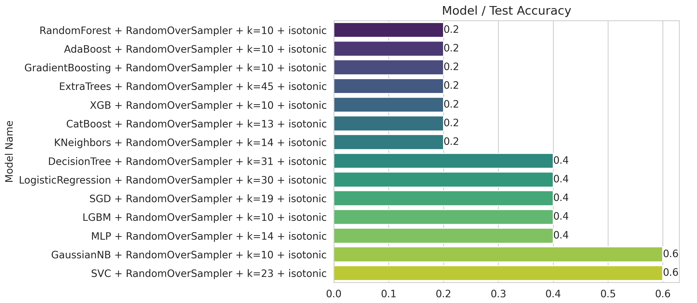
\includegraphics[width=\textwidth]{1997.png}
    \caption{1997 yılına ait model test doğrulukları.}
    \label{fig:resim1}
\end{minipage}
\hfill
\begin{minipage}[b]{0.6\textwidth}
    \centering
    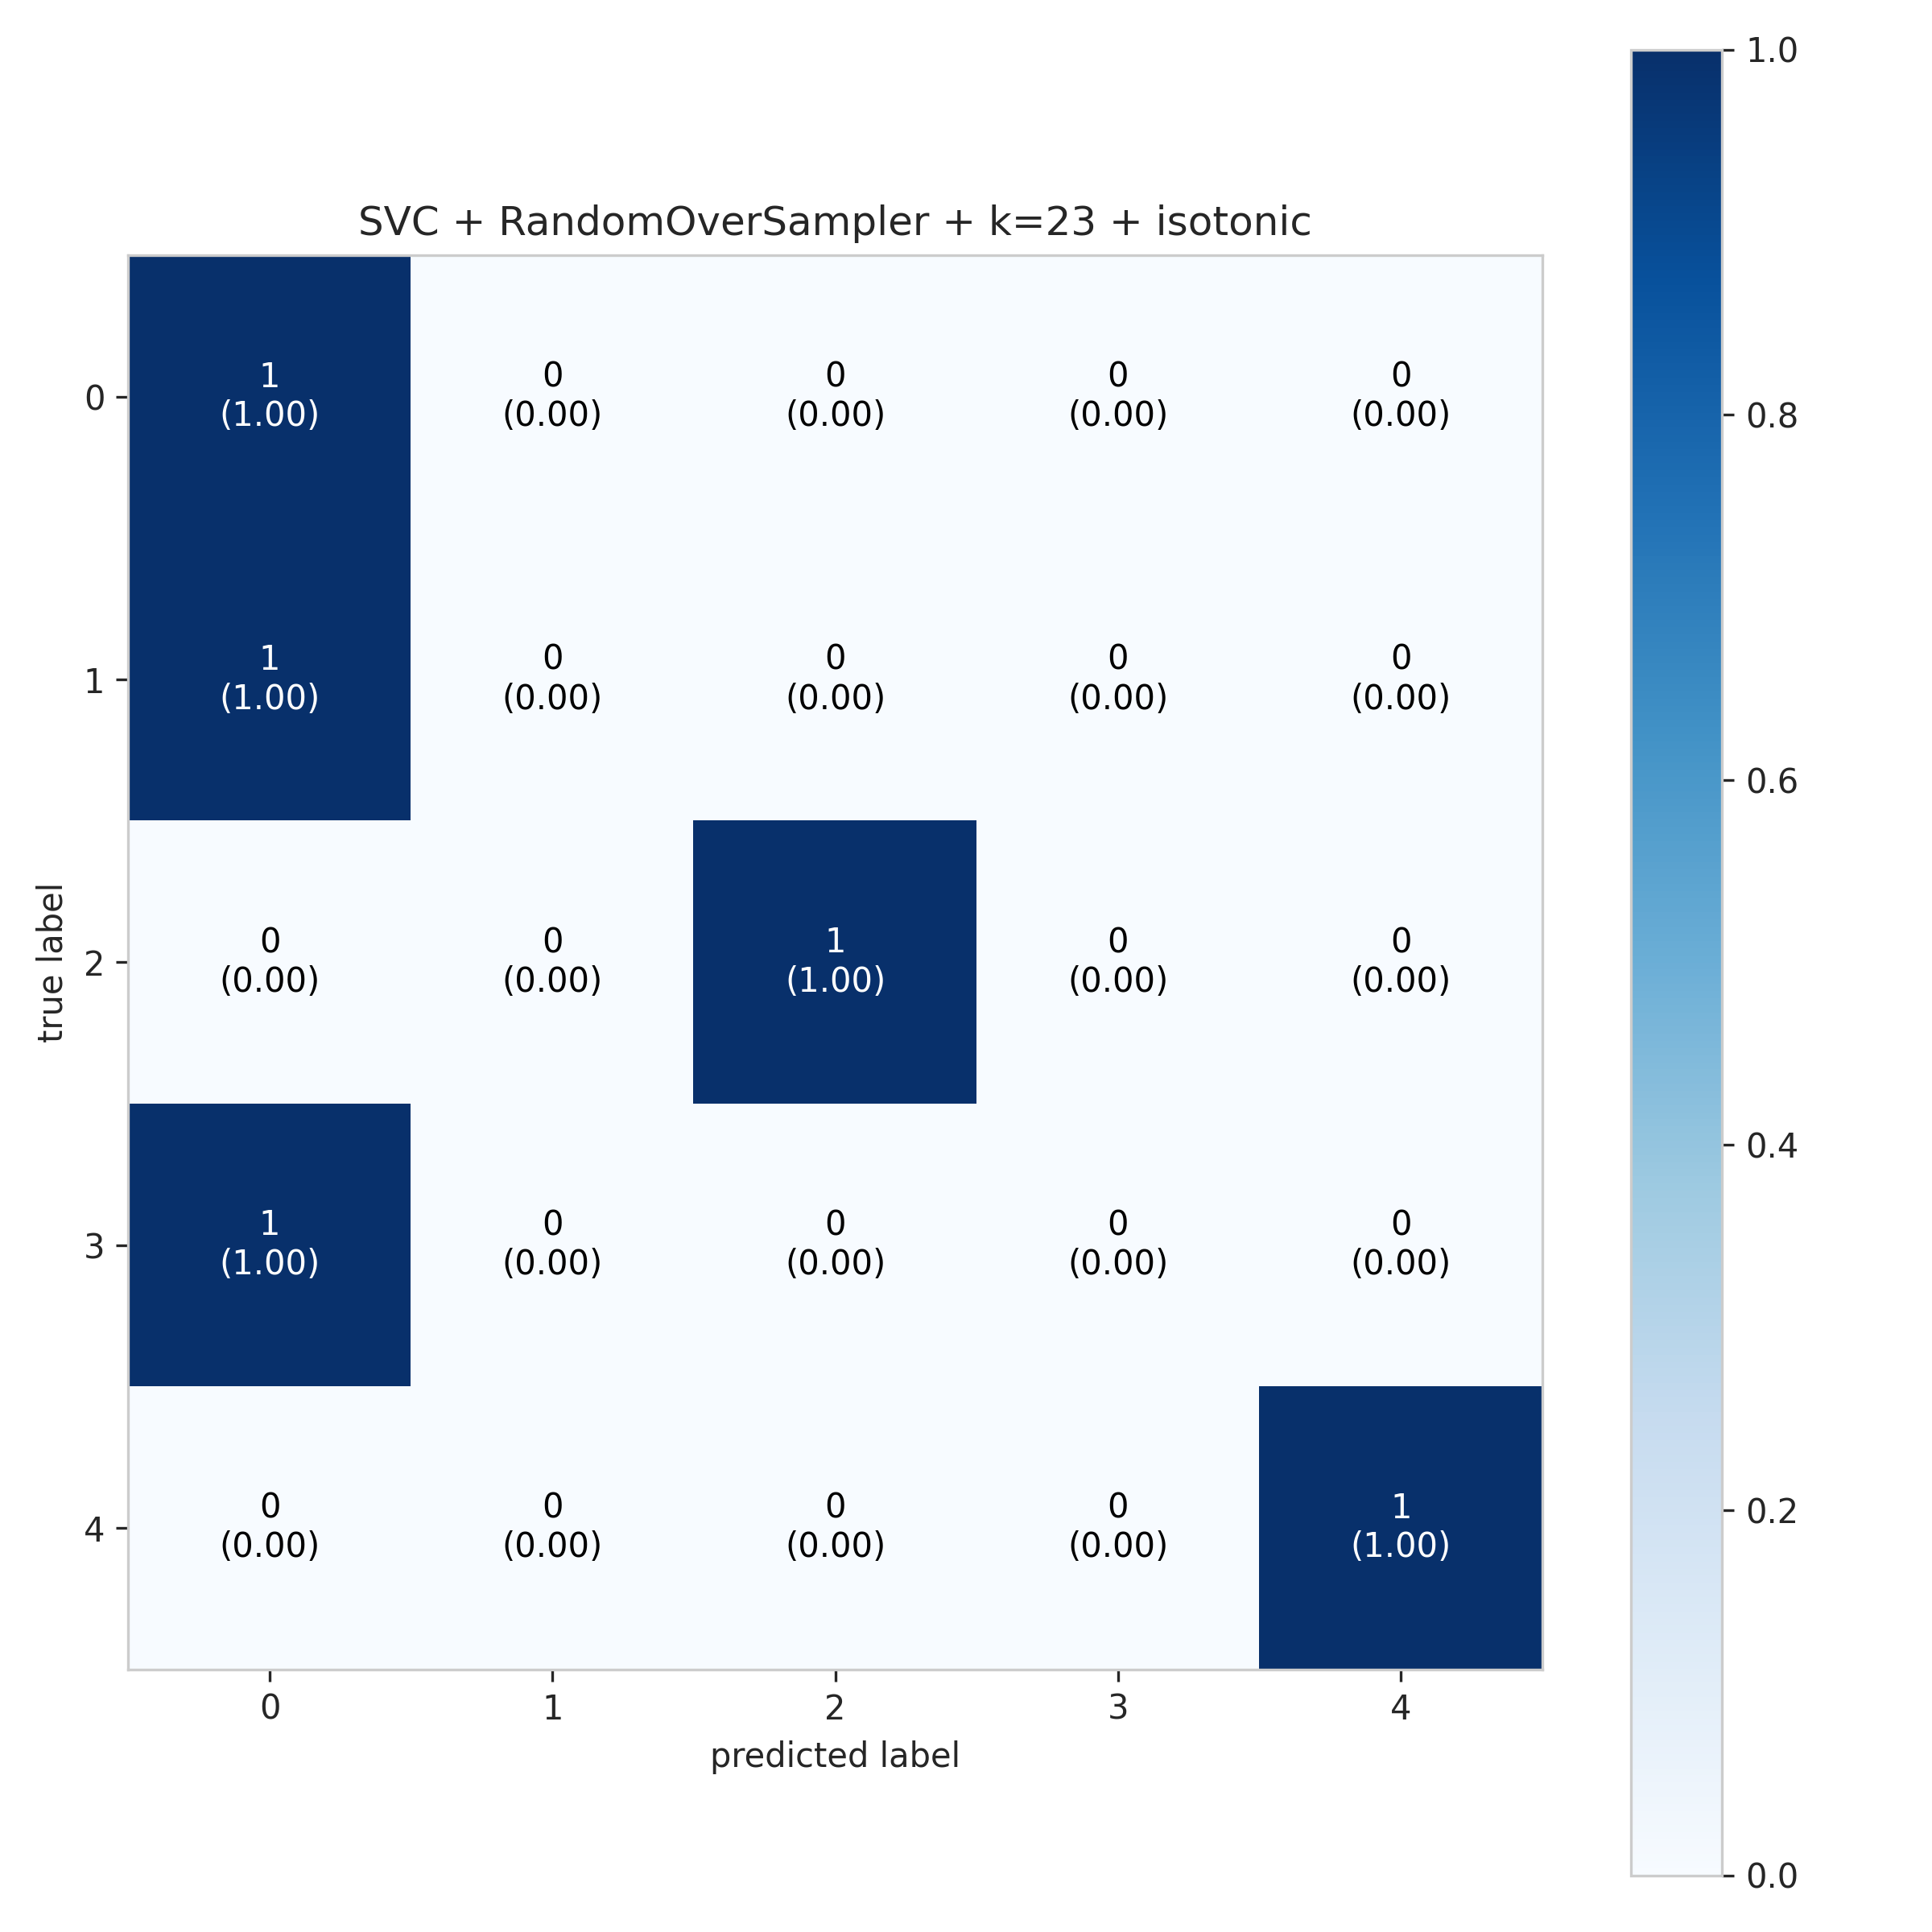
\includegraphics[width=\textwidth]{1997_cm.png}
    \caption{SVC modeline ait karmaşıklık matrisi}
    \label{fig:resim2}
\end{minipage}
\end{figure}

\newpage

\subsection{1998 yılına ait model sonuçları}
1998 yılı için en iyi performansı \%60 sınama doğruluğu,  \%50 F1 skoru, \%46.66 kesinlik skoru ve \%46.66 duyarlılık skoru ile XGB modeli vermiştir.

\begin{figure}[ht]
\centering
\begin{minipage}[b]{0.6\textwidth}
    \centering
    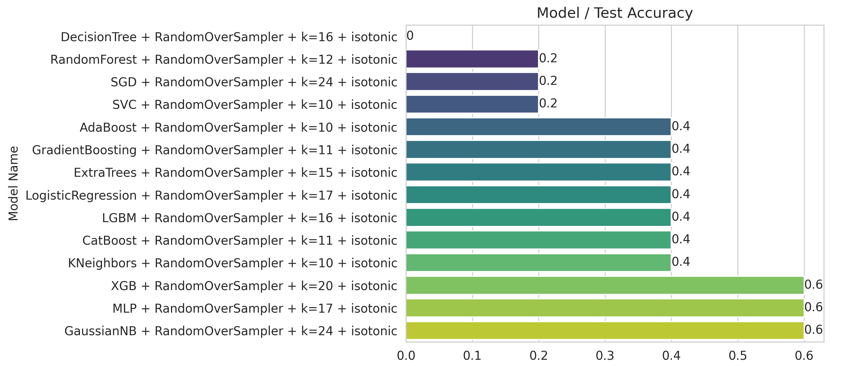
\includegraphics[width=\textwidth]{1998.png}
    \caption{1998 yılına ait model test doğrulukları.}
    \label{fig:resim1}
\end{minipage}
\hfill
\begin{minipage}[b]{0.6\textwidth}
    \centering
    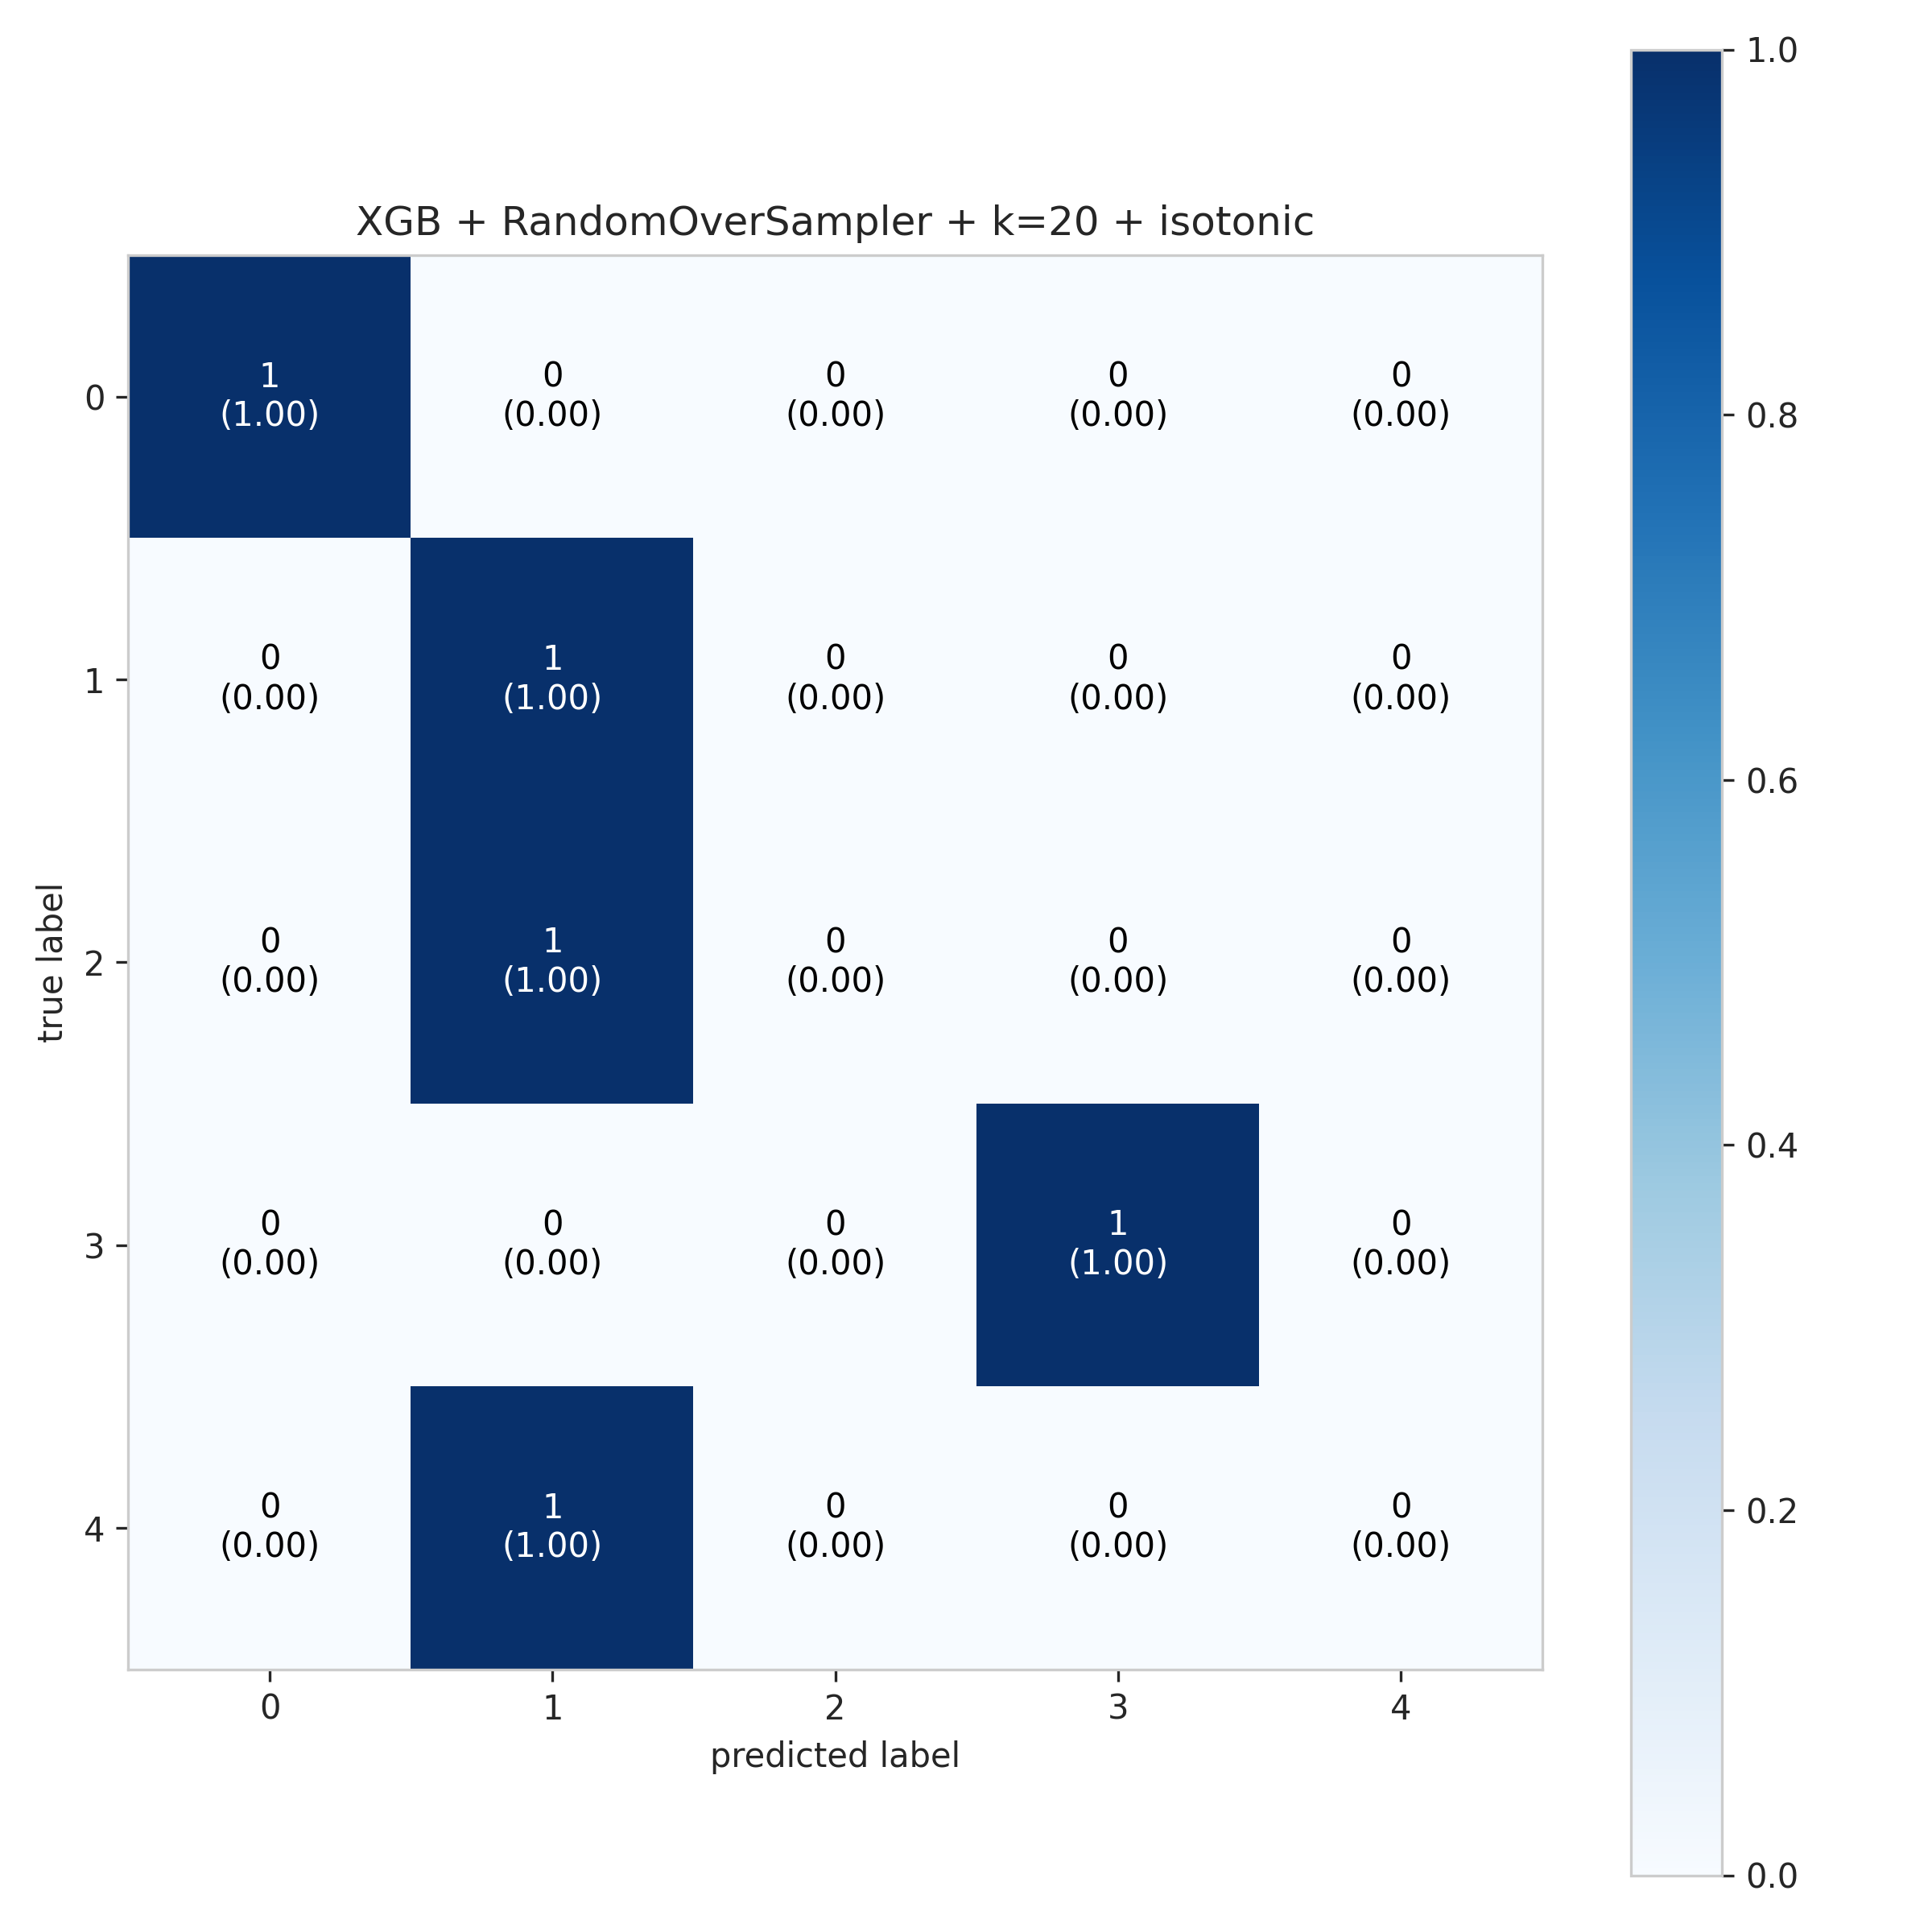
\includegraphics[width=\textwidth]{1998_cm.png}
    \caption{XGB modeline ait karmaşıklık matrisi}
    \label{fig:resim2}
\end{minipage}
\end{figure}

\newpage

\subsection{1999 yılına ait model sonuçları}
1999 yılı için en iyi performansı \%60 sınama doğruluğu,  \%53.33 F1 skoru, \%50 kesinlik skoru ve \%50 duyarlılık skoru ile Gaussian Naive Bayes modeli vermiştir.

\begin{figure}[ht]
\centering
\begin{minipage}[b]{0.6\textwidth}
    \centering
    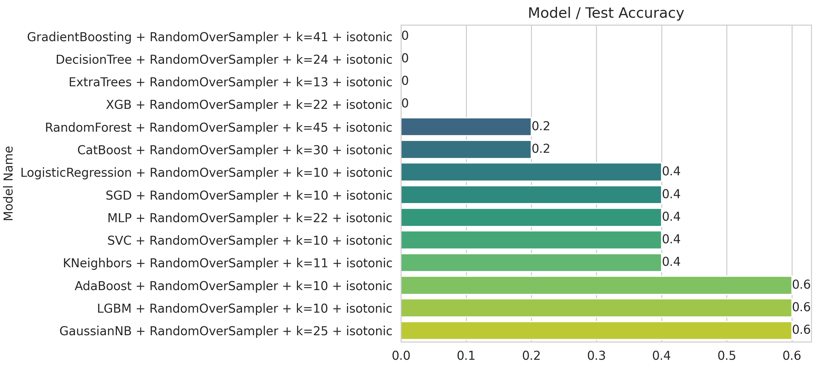
\includegraphics[width=\textwidth]{1999.png}
    \caption{1999 yılına ait model test doğrulukları.}
    \label{fig:resim1}
\end{minipage}
\hfill
\begin{minipage}[b]{0.6\textwidth}
    \centering
    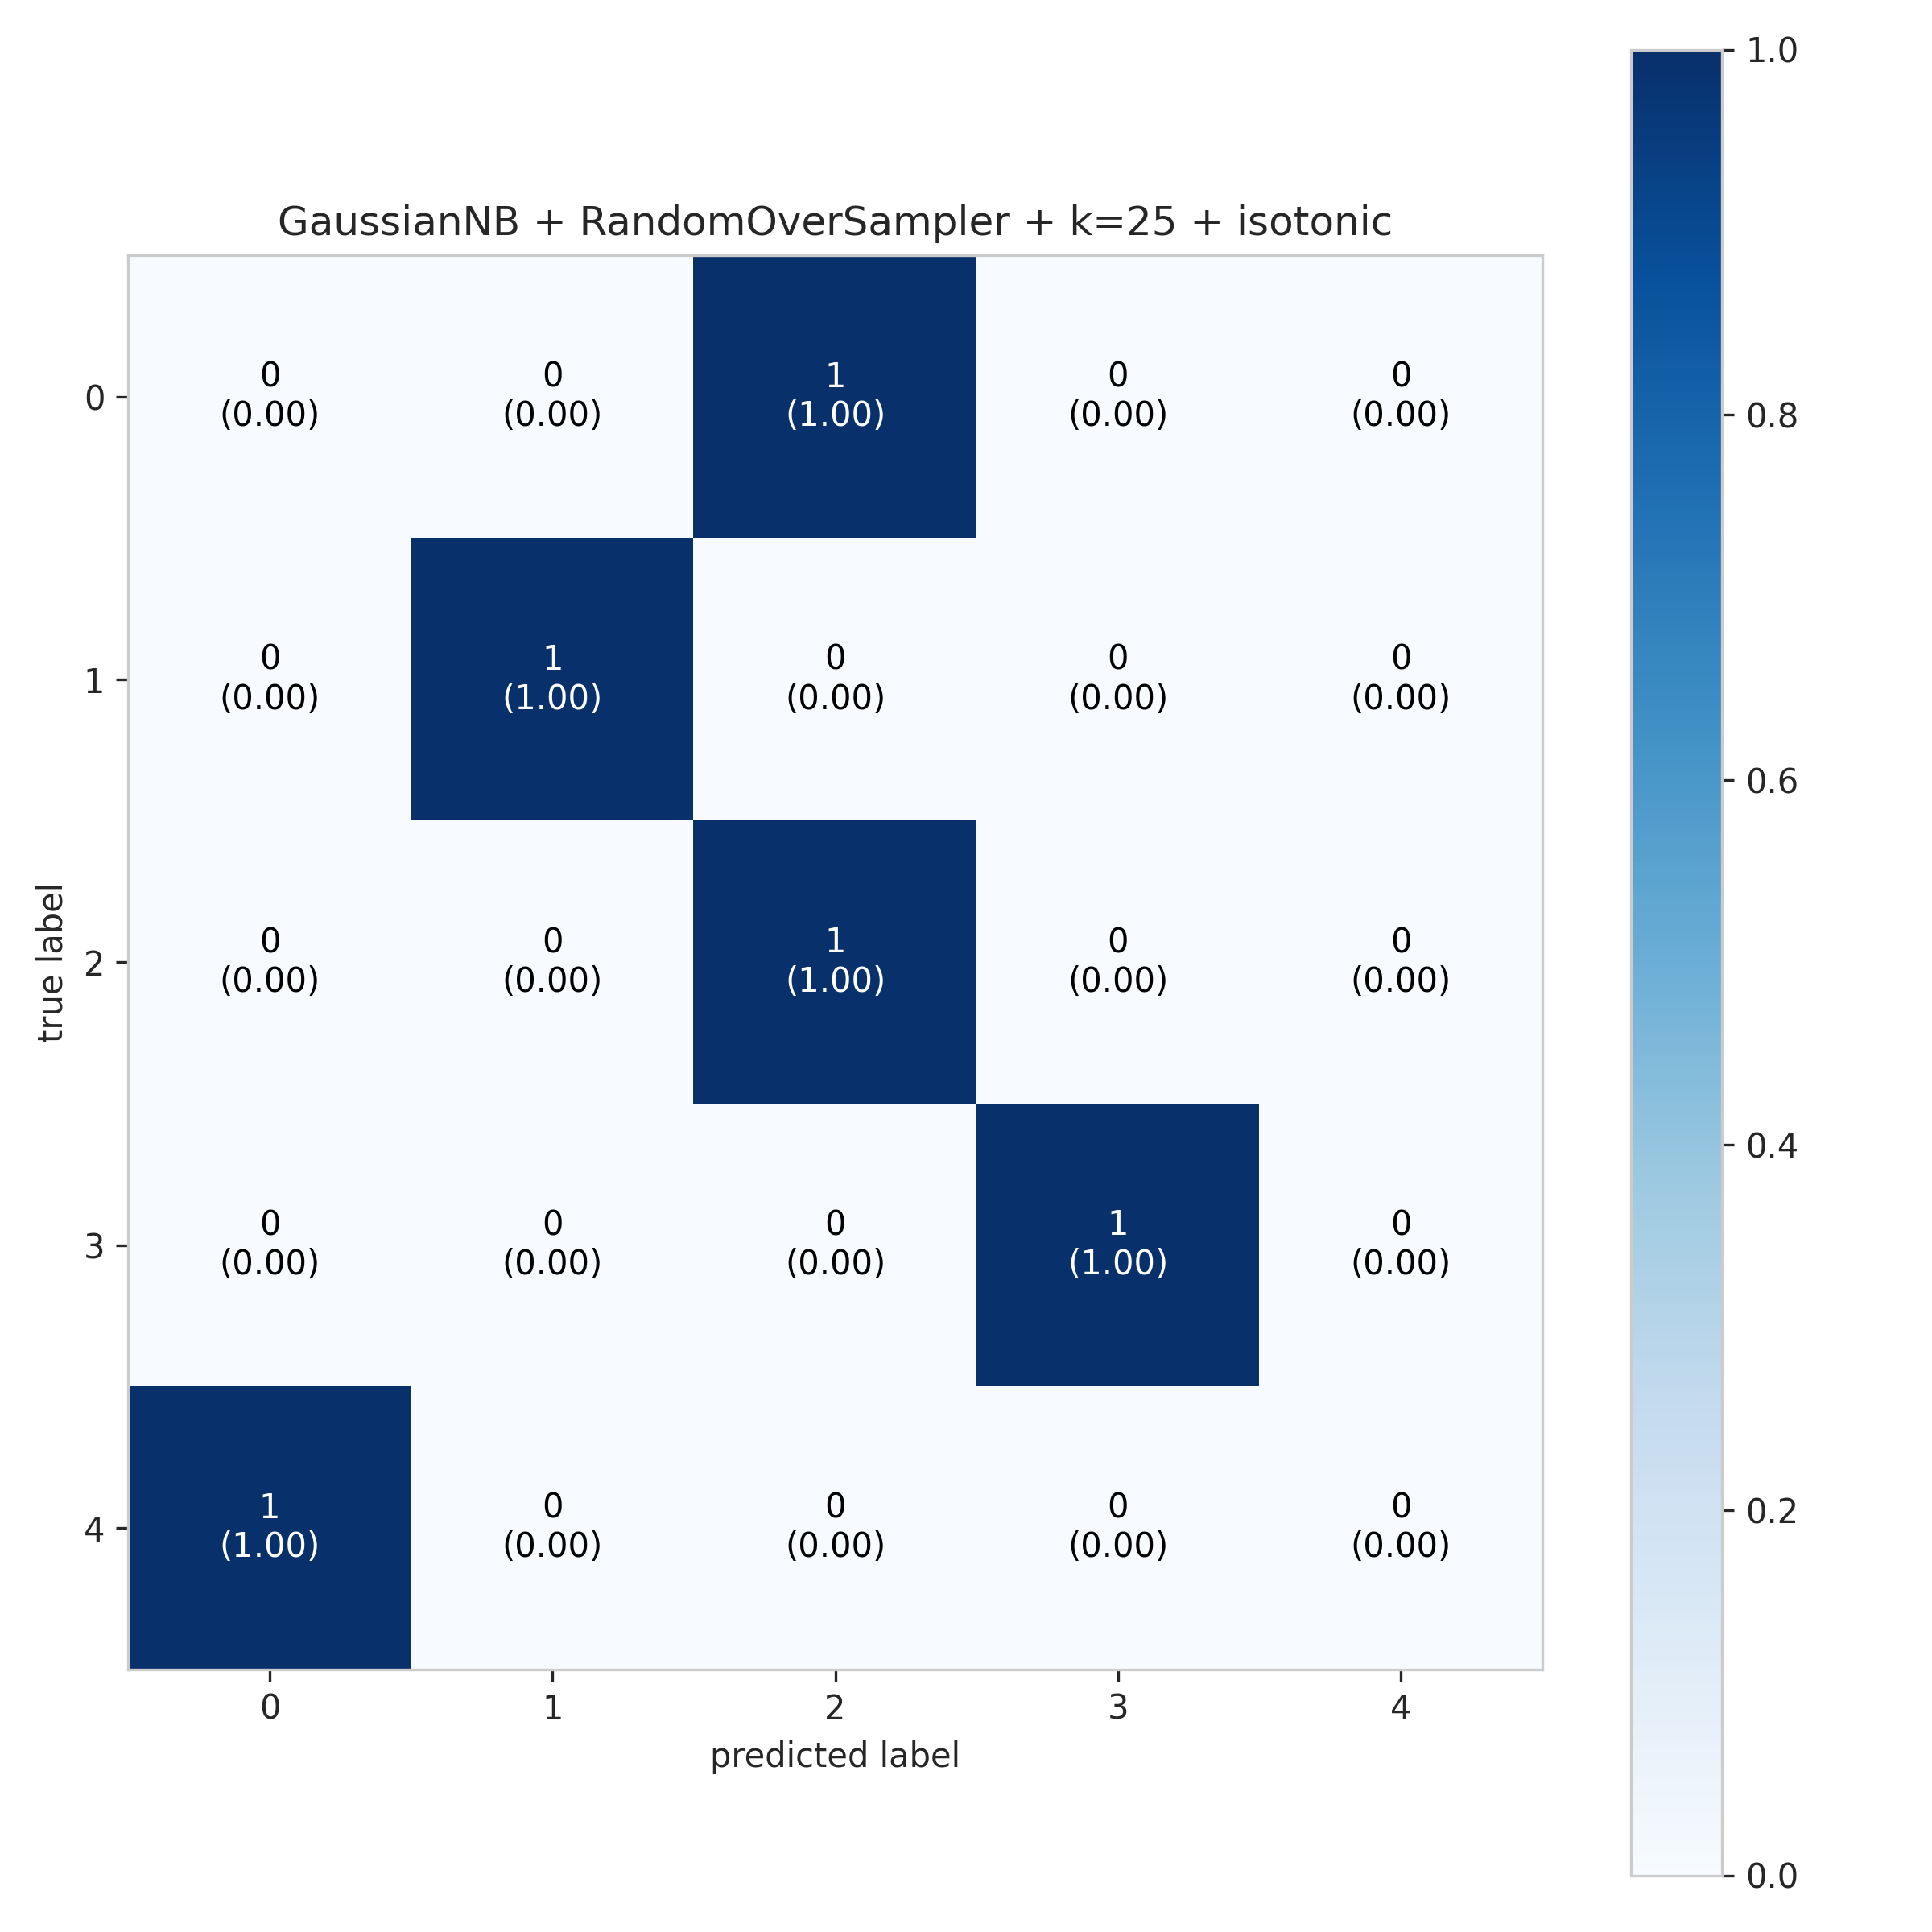
\includegraphics[width=\textwidth]{1999_cm.png}
    \caption{Gaussian Naive Bayes modeline ait karmaşıklık matrisi}
    \label{fig:resim2}
\end{minipage}
\end{figure}

\newpage

\subsection{2000 yılına ait model sonuçları}
2000 yılı için en iyi performansı \%40 sınama doğruluğu,  \%32 F1 skoru, \%26.66 kesinlik skoru ve \%26.66 duyarlılık skoru ile SVC modeli vermiştir.

\begin{figure}[ht]
\centering
\begin{minipage}[b]{0.6\textwidth}
    \centering
    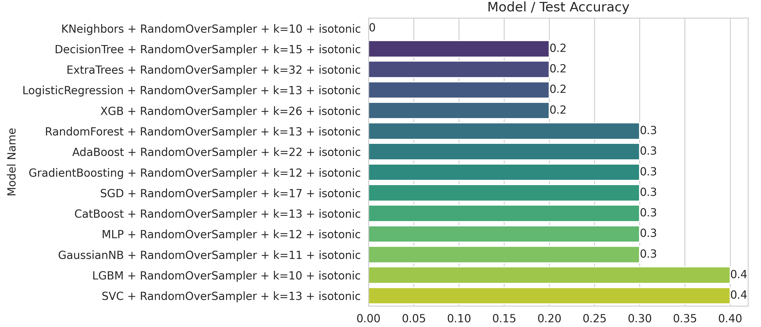
\includegraphics[width=\textwidth]{2000.png}
    \caption{2000 yılına ait model test doğrulukları.}
    \label{fig:resim1}
\end{minipage}
\hfill
\begin{minipage}[b]{0.6\textwidth}
    \centering
    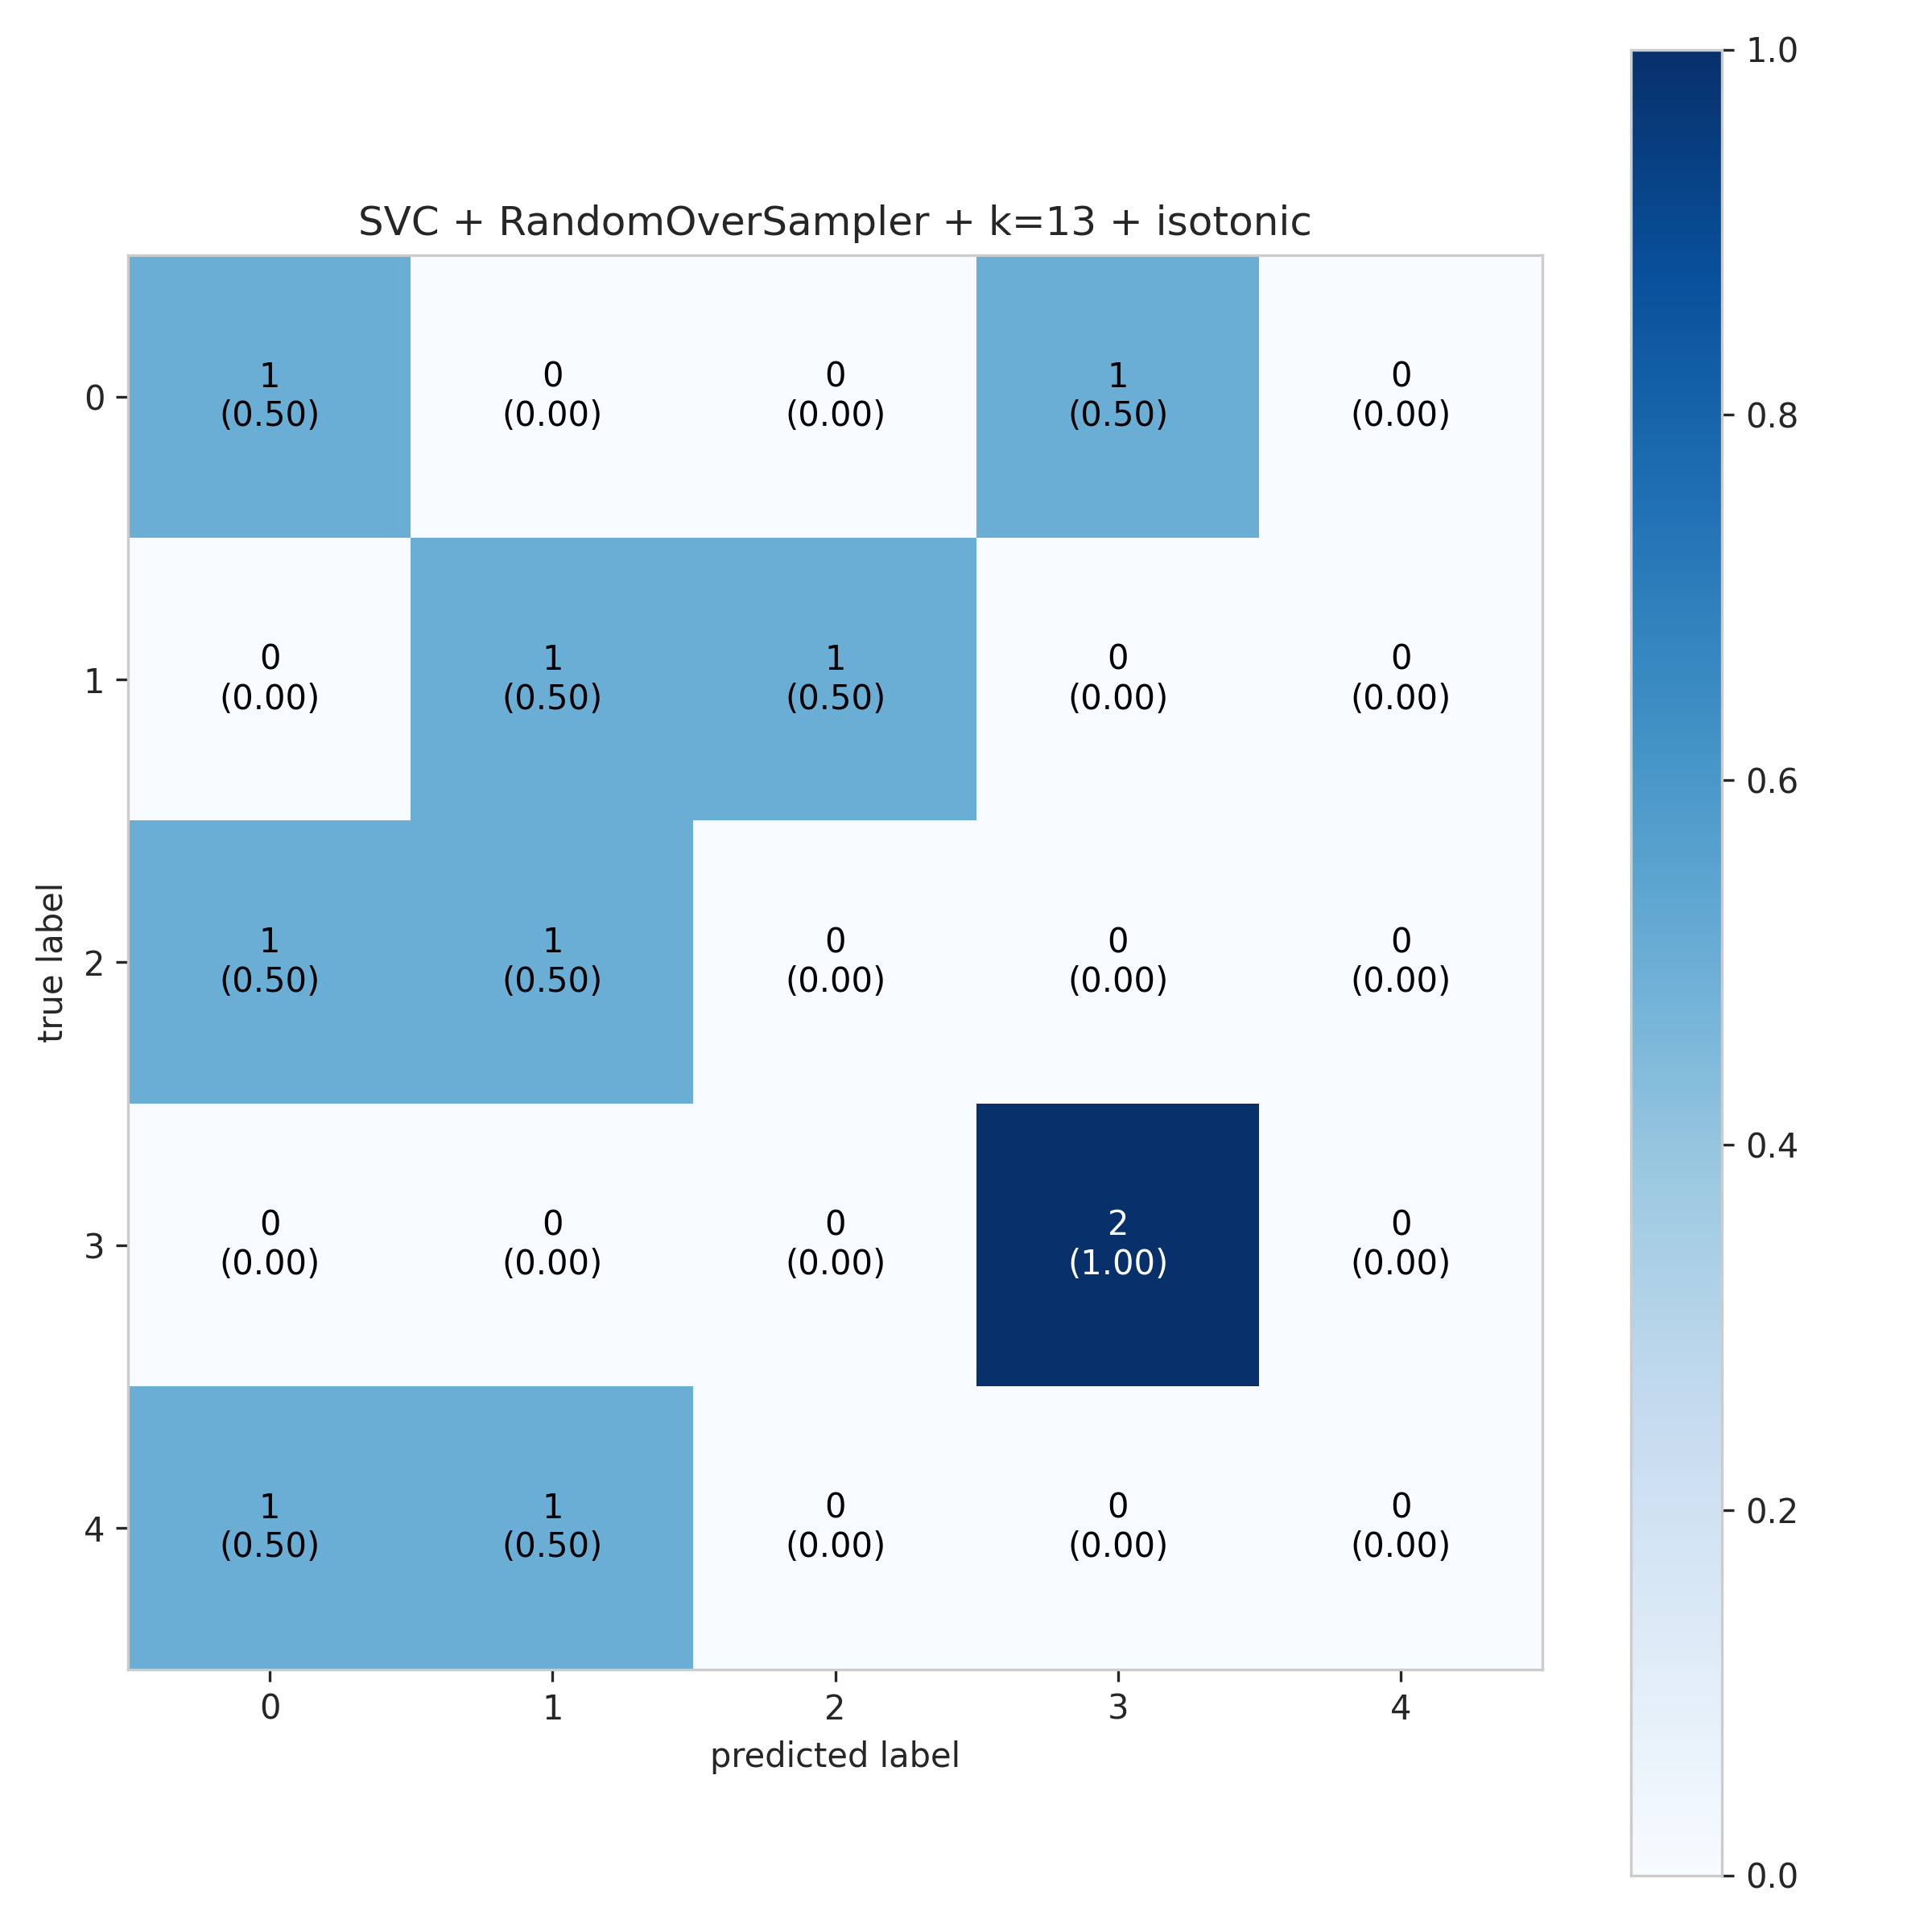
\includegraphics[width=\textwidth]{2000_cm.png}
    \caption{SVC modeline ait karmaşıklık matrisi}
    \label{fig:resim2}
\end{minipage}
\end{figure}

\newpage

\subsection{2001 yılına ait model sonuçları}
2001 yılı için en iyi performansı \%50 sınama doğruluğu,  \%44.76 F1 skoru, \%48 kesinlik skoru ve \%48 duyarlılık skoru ile CatBoost modeli vermiştir.

\begin{figure}[ht]
\centering
\begin{minipage}[b]{0.6\textwidth}
    \centering
    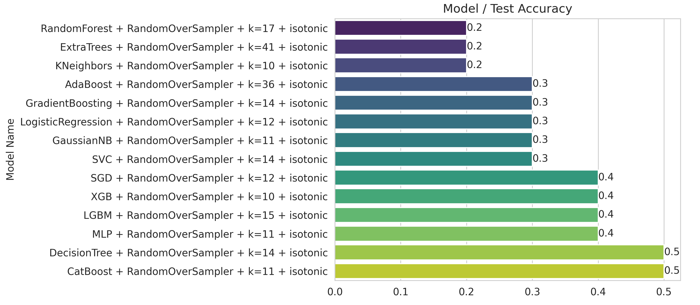
\includegraphics[width=\textwidth]{2001.png}
    \caption{2001 yılına ait model test doğrulukları.}
    \label{fig:resim1}
\end{minipage}
\hfill
\begin{minipage}[b]{0.6\textwidth}
    \centering
    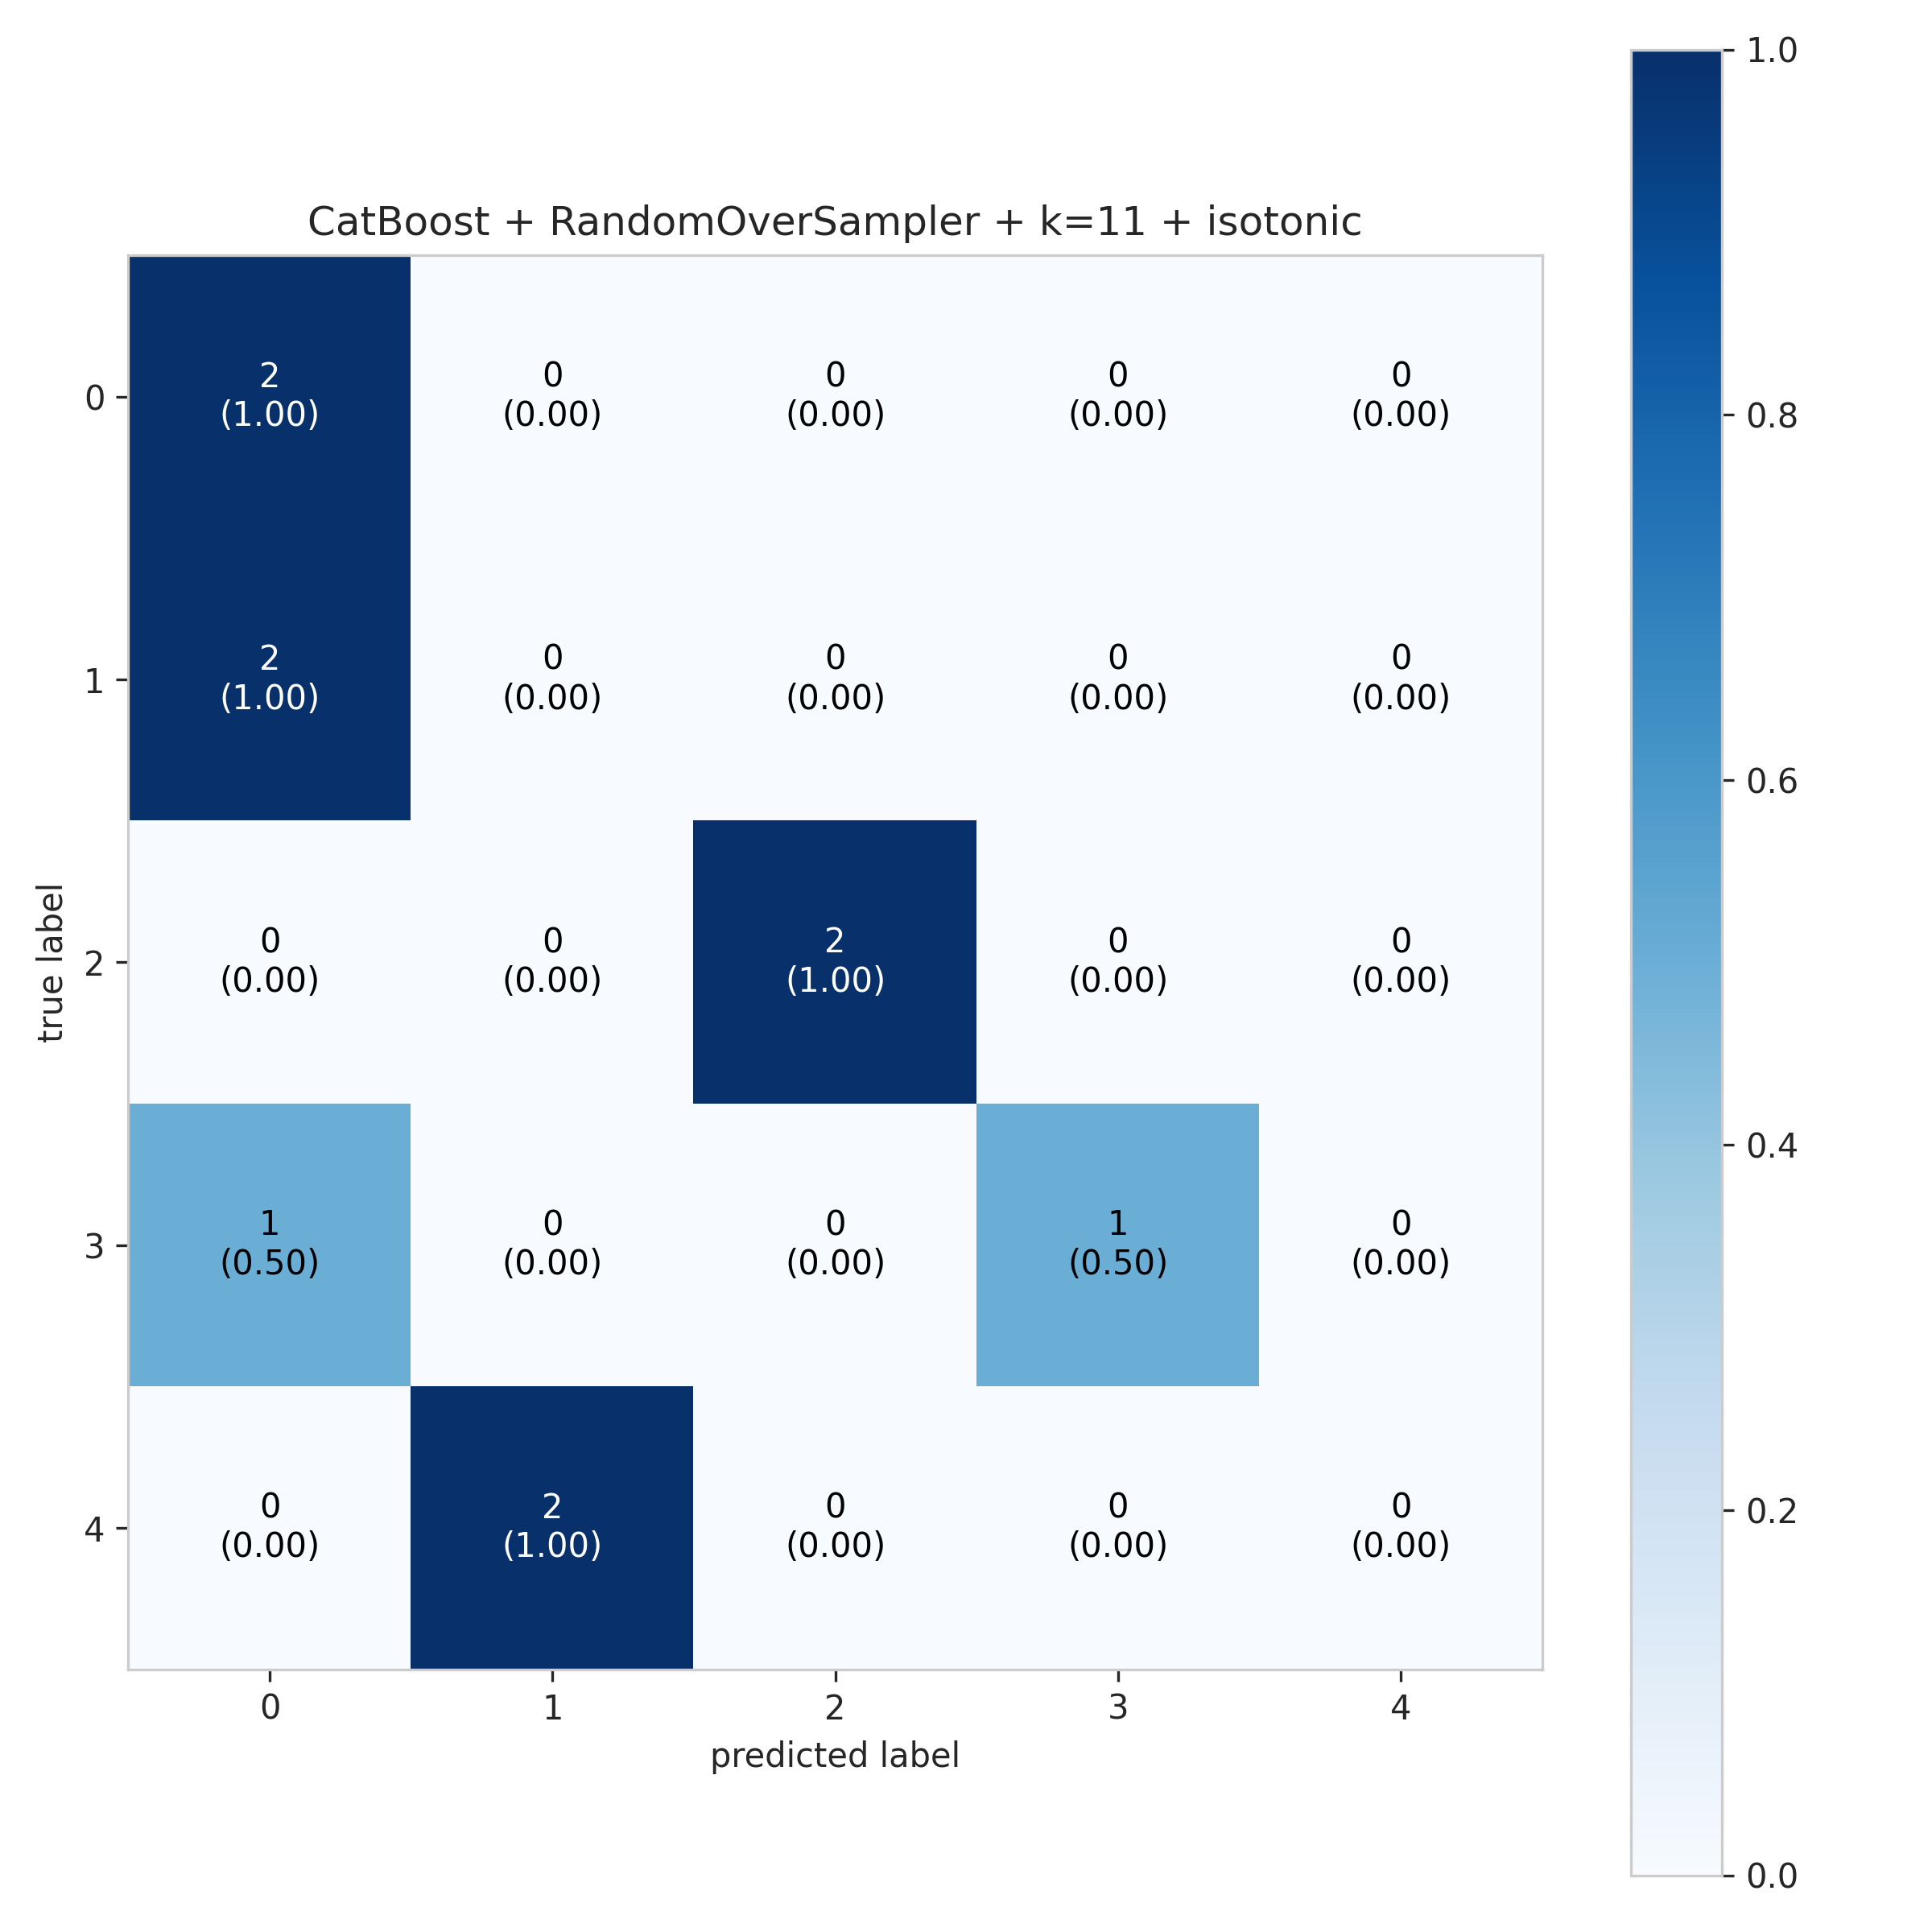
\includegraphics[width=\textwidth]{2001_cm.png}
    \caption{CatBoost modeline ait karmaşıklık matrisi}
    \label{fig:resim2}
\end{minipage}
\end{figure}

\newpage

\subsection{2002 yılına ait model sonuçları}
2002 yılı için en iyi performansı \%60 sınama doğruluğu,  \%61.33 F1 skoru, \%76.66 kesinlik skoru ve \%76.66 duyarlılık skoru ile Logistic Regression modeli vermiştir.

\begin{figure}[ht]
\centering
\begin{minipage}[b]{0.6\textwidth}
    \centering
    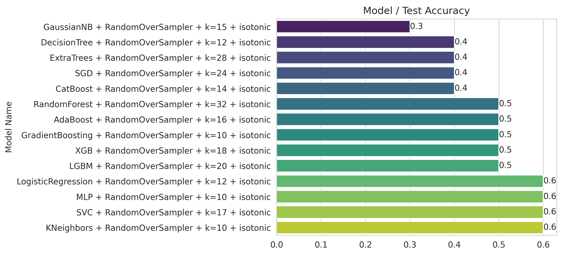
\includegraphics[width=\textwidth]{2002.png}
    \caption{2002 yılına ait model test doğrulukları.}
    \label{fig:resim1}
\end{minipage}
\hfill
\begin{minipage}[b]{0.6\textwidth}
    \centering
    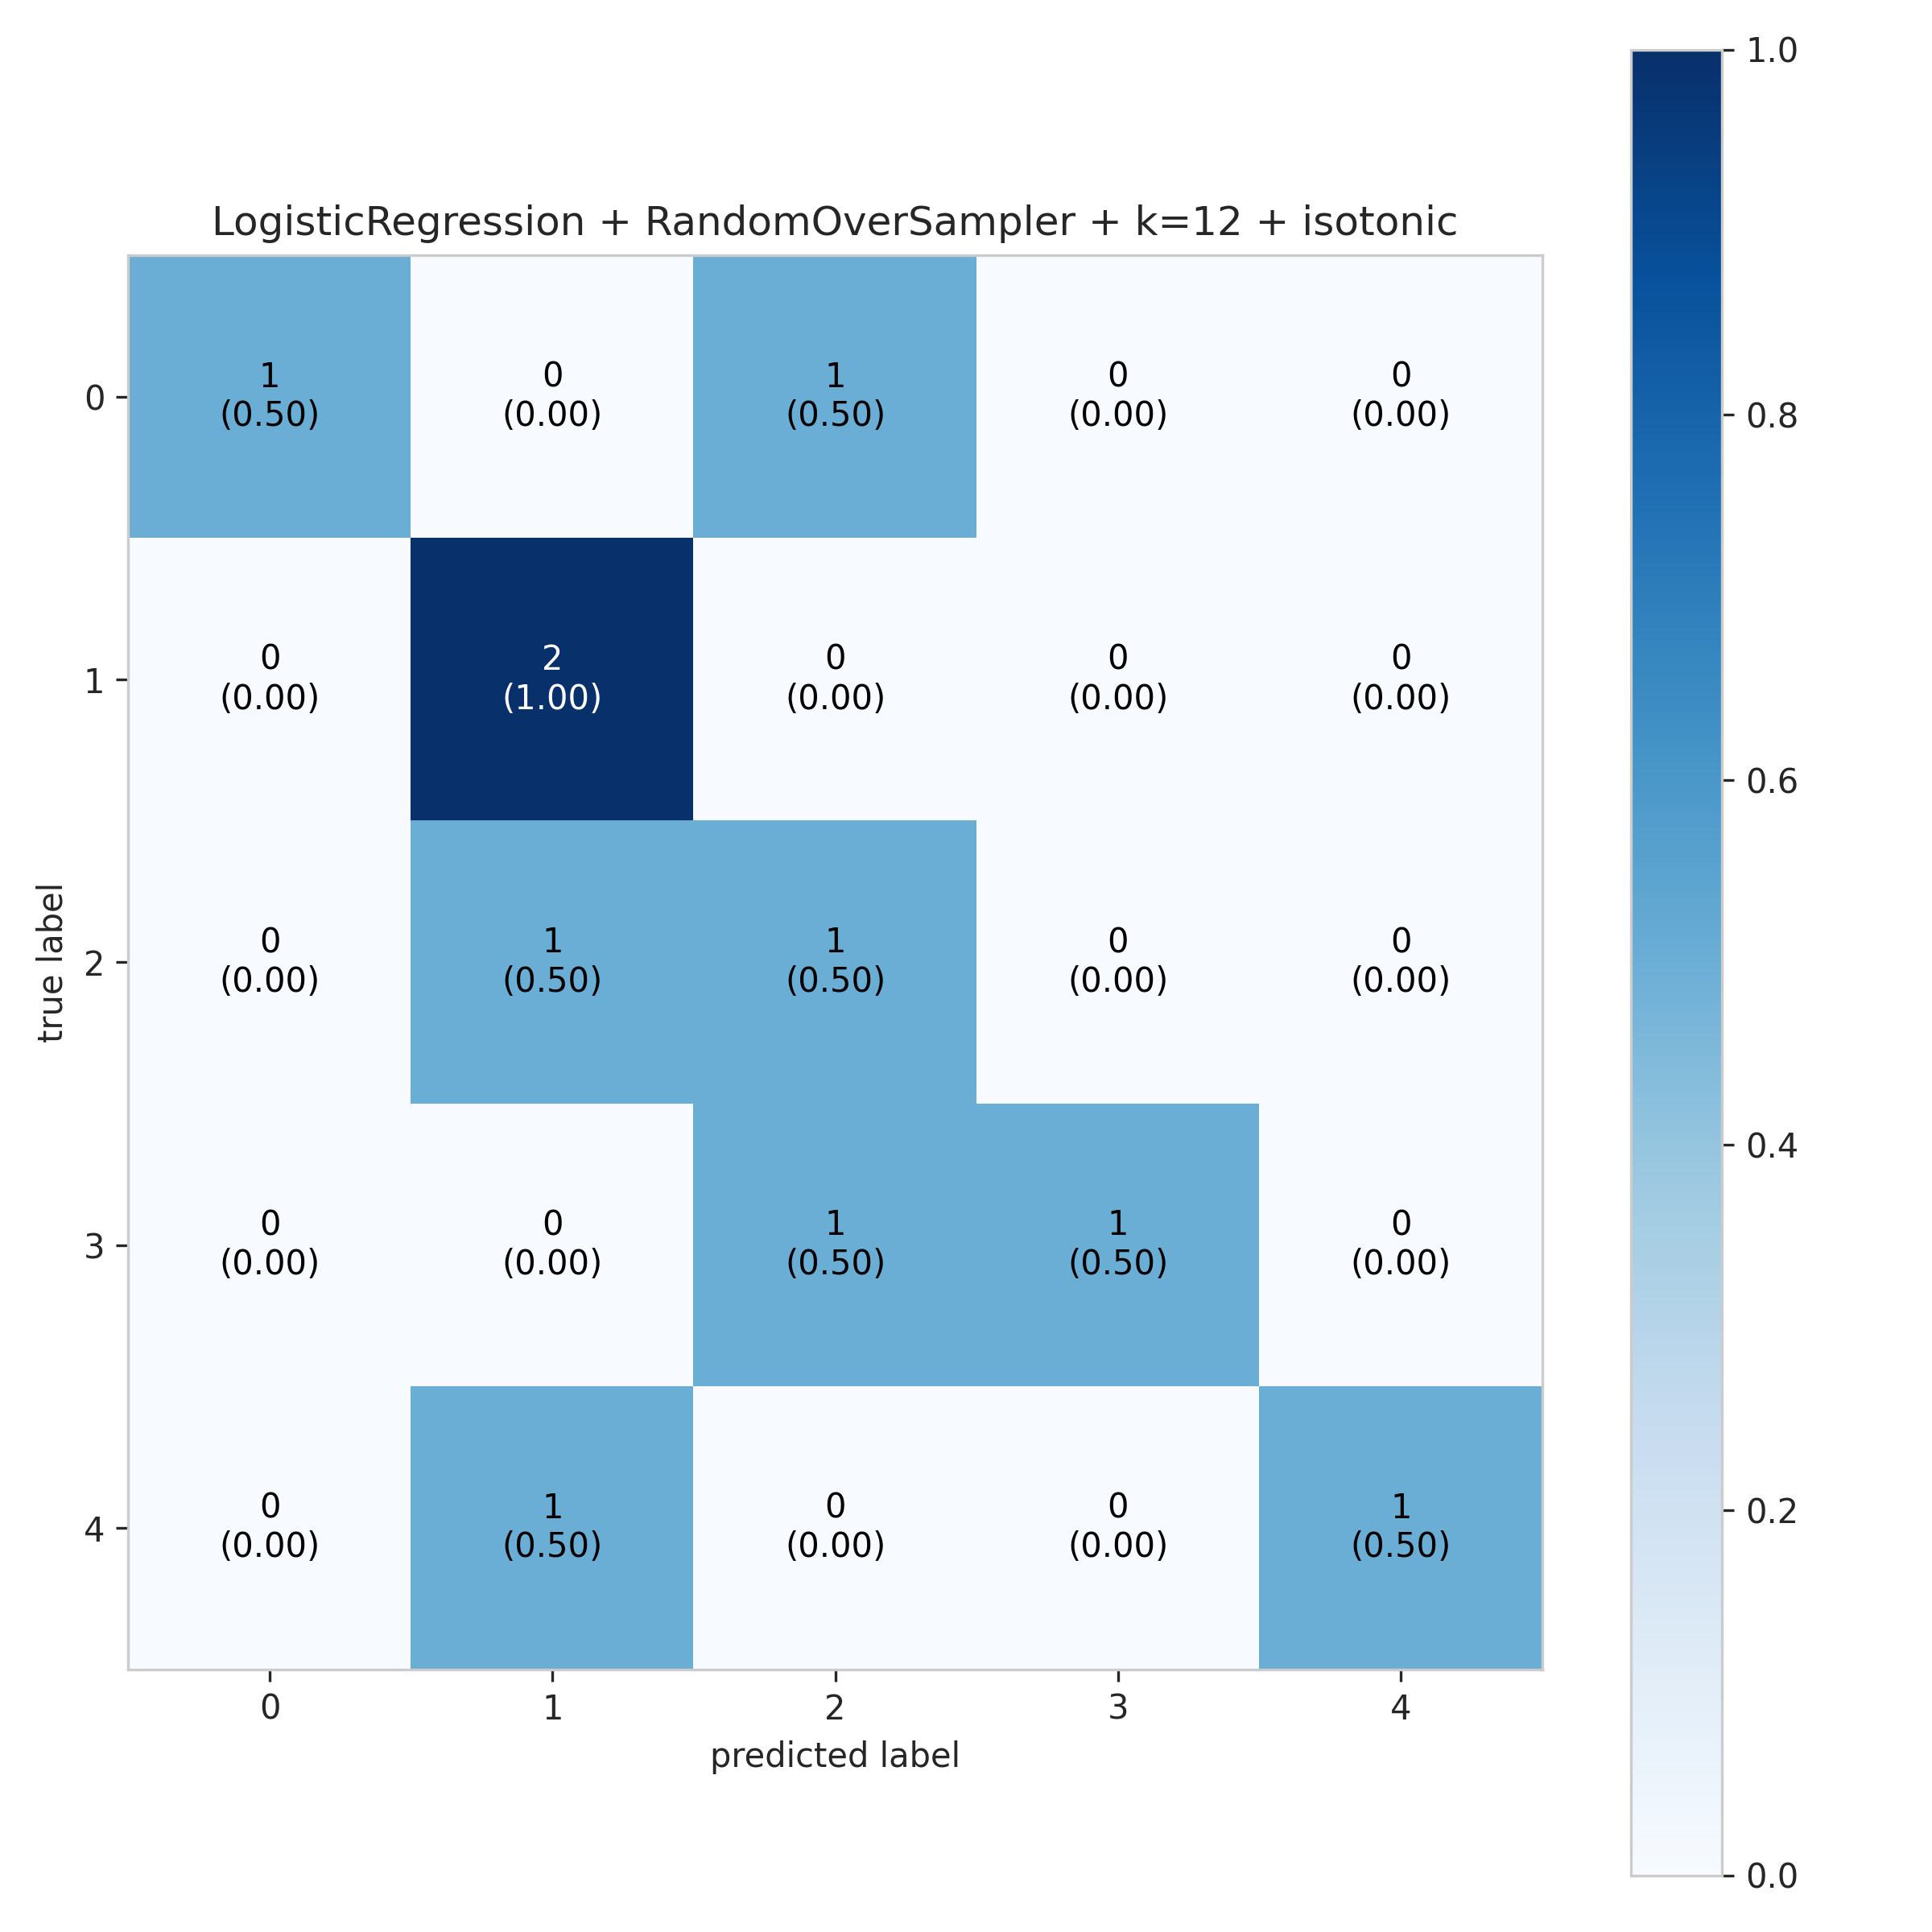
\includegraphics[width=\textwidth]{2002_cm.png}
    \caption{Logistic Regression modeline ait karmaşıklık matrisi}
    \label{fig:resim2}
\end{minipage}
\end{figure}

\newpage

\subsection{2003 yılına ait model sonuçları}
2003 yılı için en iyi performansı \%70 sınama doğruluğu,  \%62 F1 skoru, \%56.66 kesinlik skoru ve \%56.66 duyarlılık skoru ile SVC modeli vermiştir.

\begin{figure}[ht]
\centering
\begin{minipage}[b]{0.7\textwidth}
    \centering
    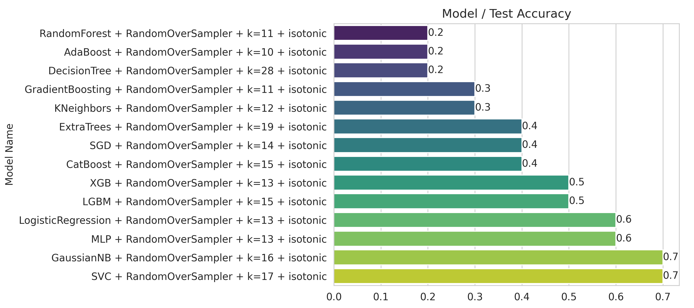
\includegraphics[width=\textwidth]{2003.png}
    \caption{2003 yılına ait model test doğrulukları.}
    \label{fig:resim1}
\end{minipage}
\hfill
\begin{minipage}[b]{0.6\textwidth}
    \centering
    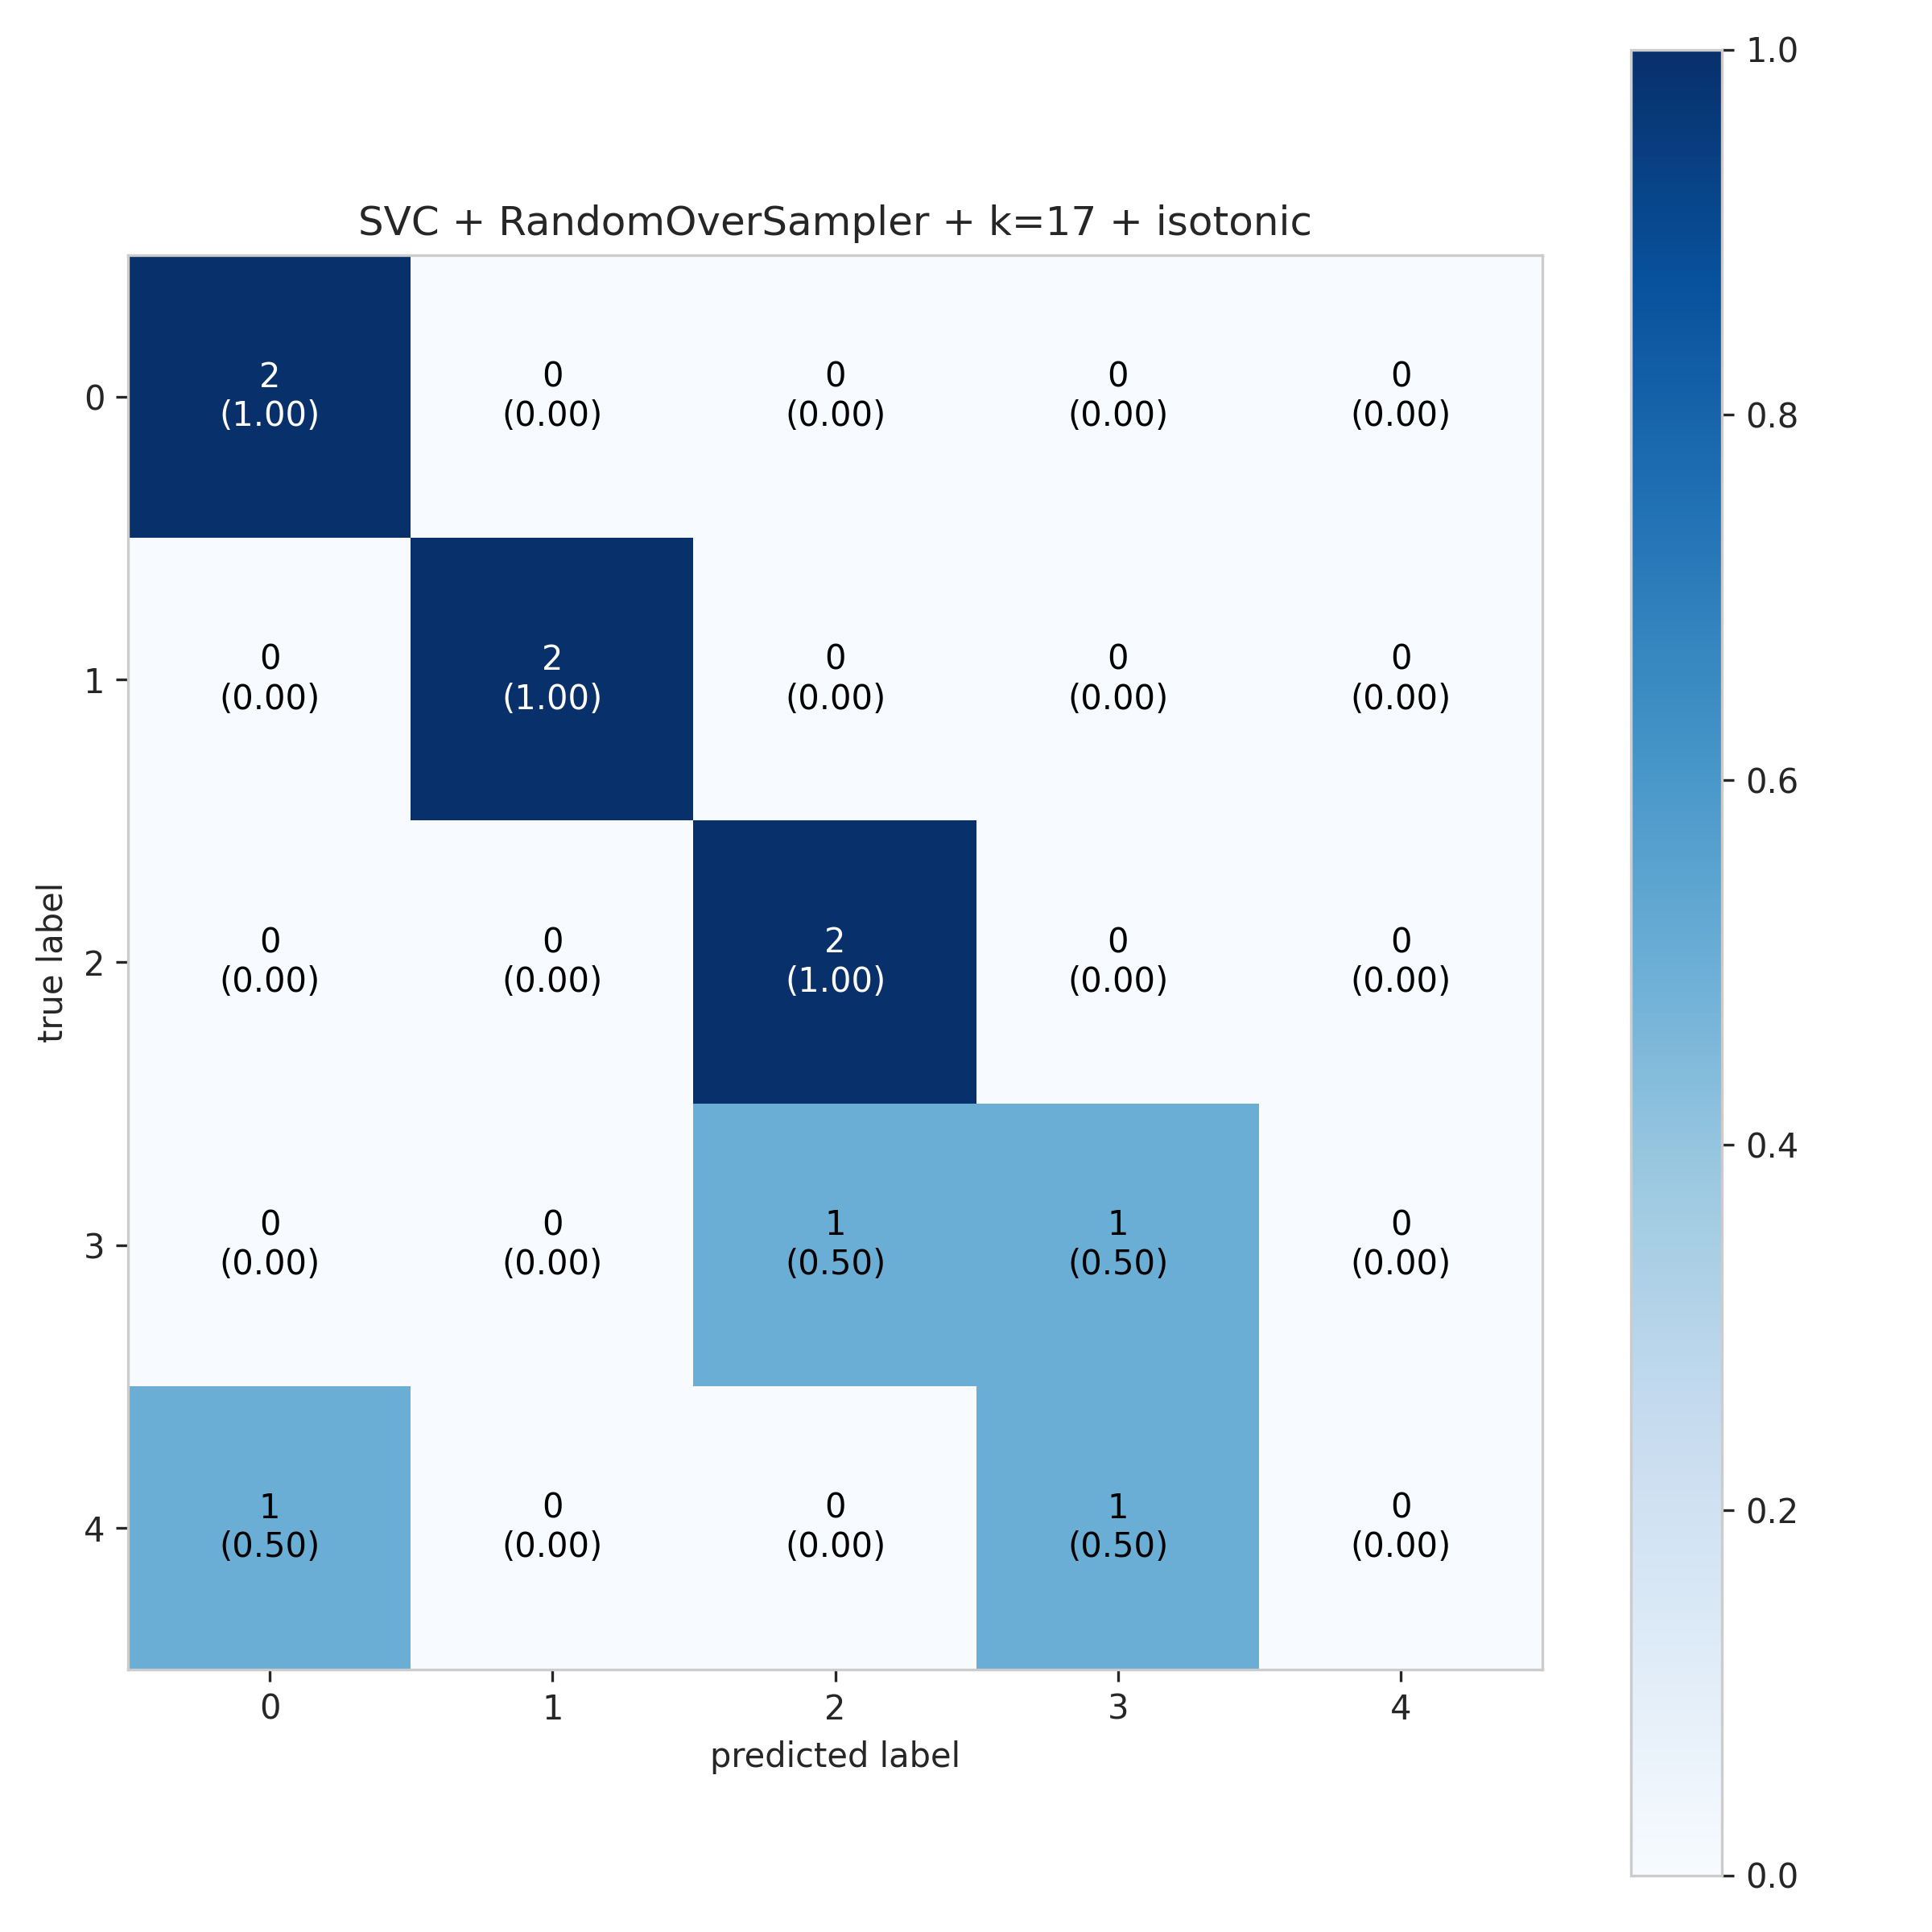
\includegraphics[width=\textwidth]{2003_cm.png}
    \caption{SVC modeline ait karmaşıklık matrisi}
    \label{fig:resim2}
\end{minipage}
\end{figure}

\newpage

\subsection{2004 yılına ait model sonuçları}
2004 yılı için en iyi performansı \%40 sınama doğruluğu,  \%40.38 F1 skoru, \%50.66 kesinlik skoru ve \%50.66 duyarlılık skoru ile SVC modeli vermiştir.

\begin{figure}[ht]
\centering
\begin{minipage}[b]{0.6\textwidth}
    \centering
    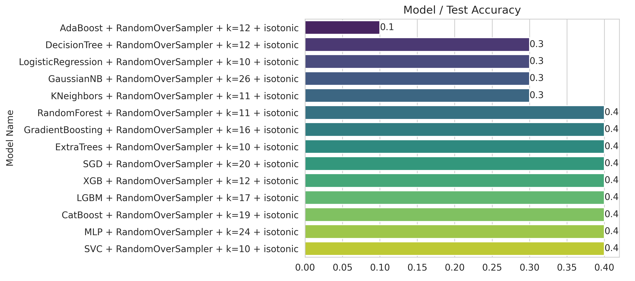
\includegraphics[width=\textwidth]{2004.png}
    \caption{2004 yılına ait model test doğrulukları.}
    \label{fig:resim1}
\end{minipage}
\hfill
\begin{minipage}[b]{0.6\textwidth}
    \centering
    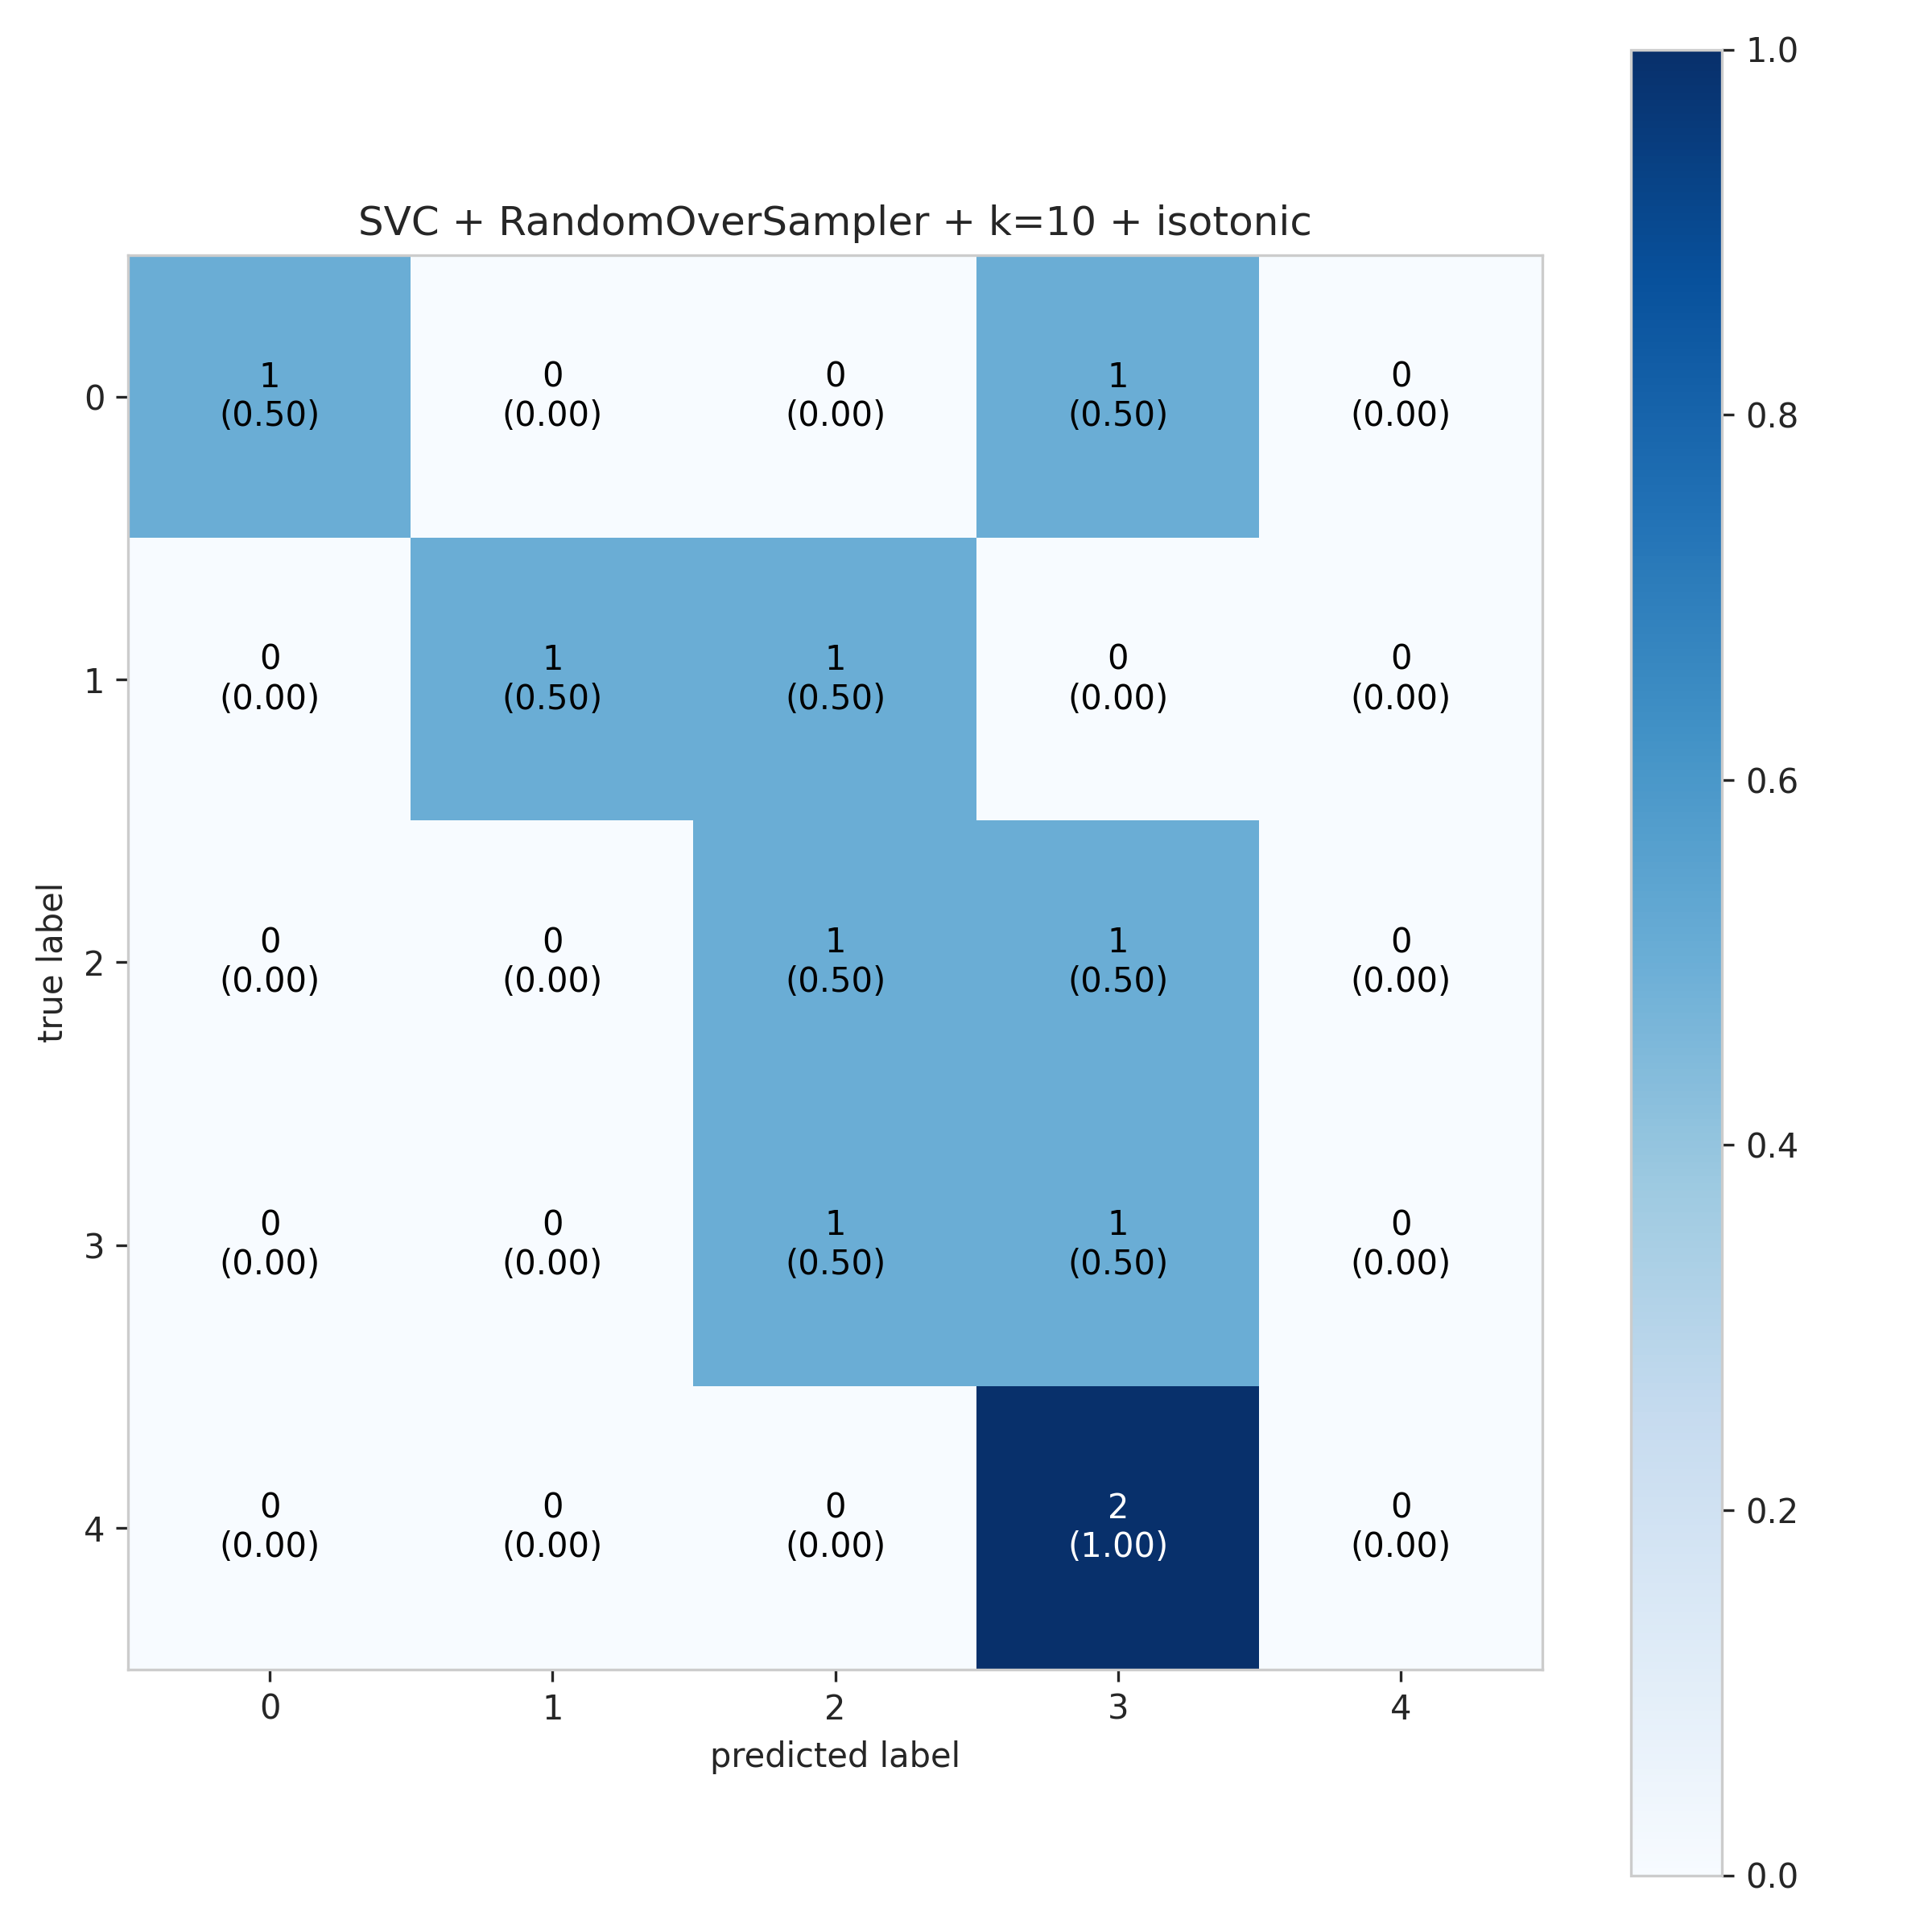
\includegraphics[width=\textwidth]{2004_cm.png}
    \caption{SVC modeline ait karmaşıklık matrisi}
    \label{fig:resim2}
\end{minipage}
\end{figure}

\newpage

\subsection{2005 yılına ait model sonuçları}
2005 yılı için en iyi performansı \%60 sınama doğruluğu,  \%47.42 F1 skoru, \%41.33 kesinlik skoru ve \%41.33 duyarlılık skoru ile Gradient Boosting modeli vermiştir.

\begin{figure}[ht]
\centering
\begin{minipage}[b]{0.6\textwidth}
    \centering
    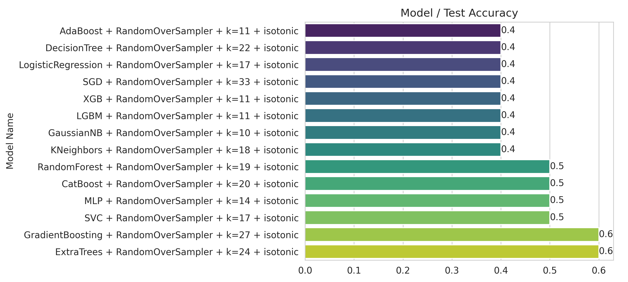
\includegraphics[width=\textwidth]{2005.png}
    \caption{2005 yılına ait model test doğrulukları.}
    \label{fig:resim1}
\end{minipage}
\hfill
\begin{minipage}[b]{0.6\textwidth}
    \centering
    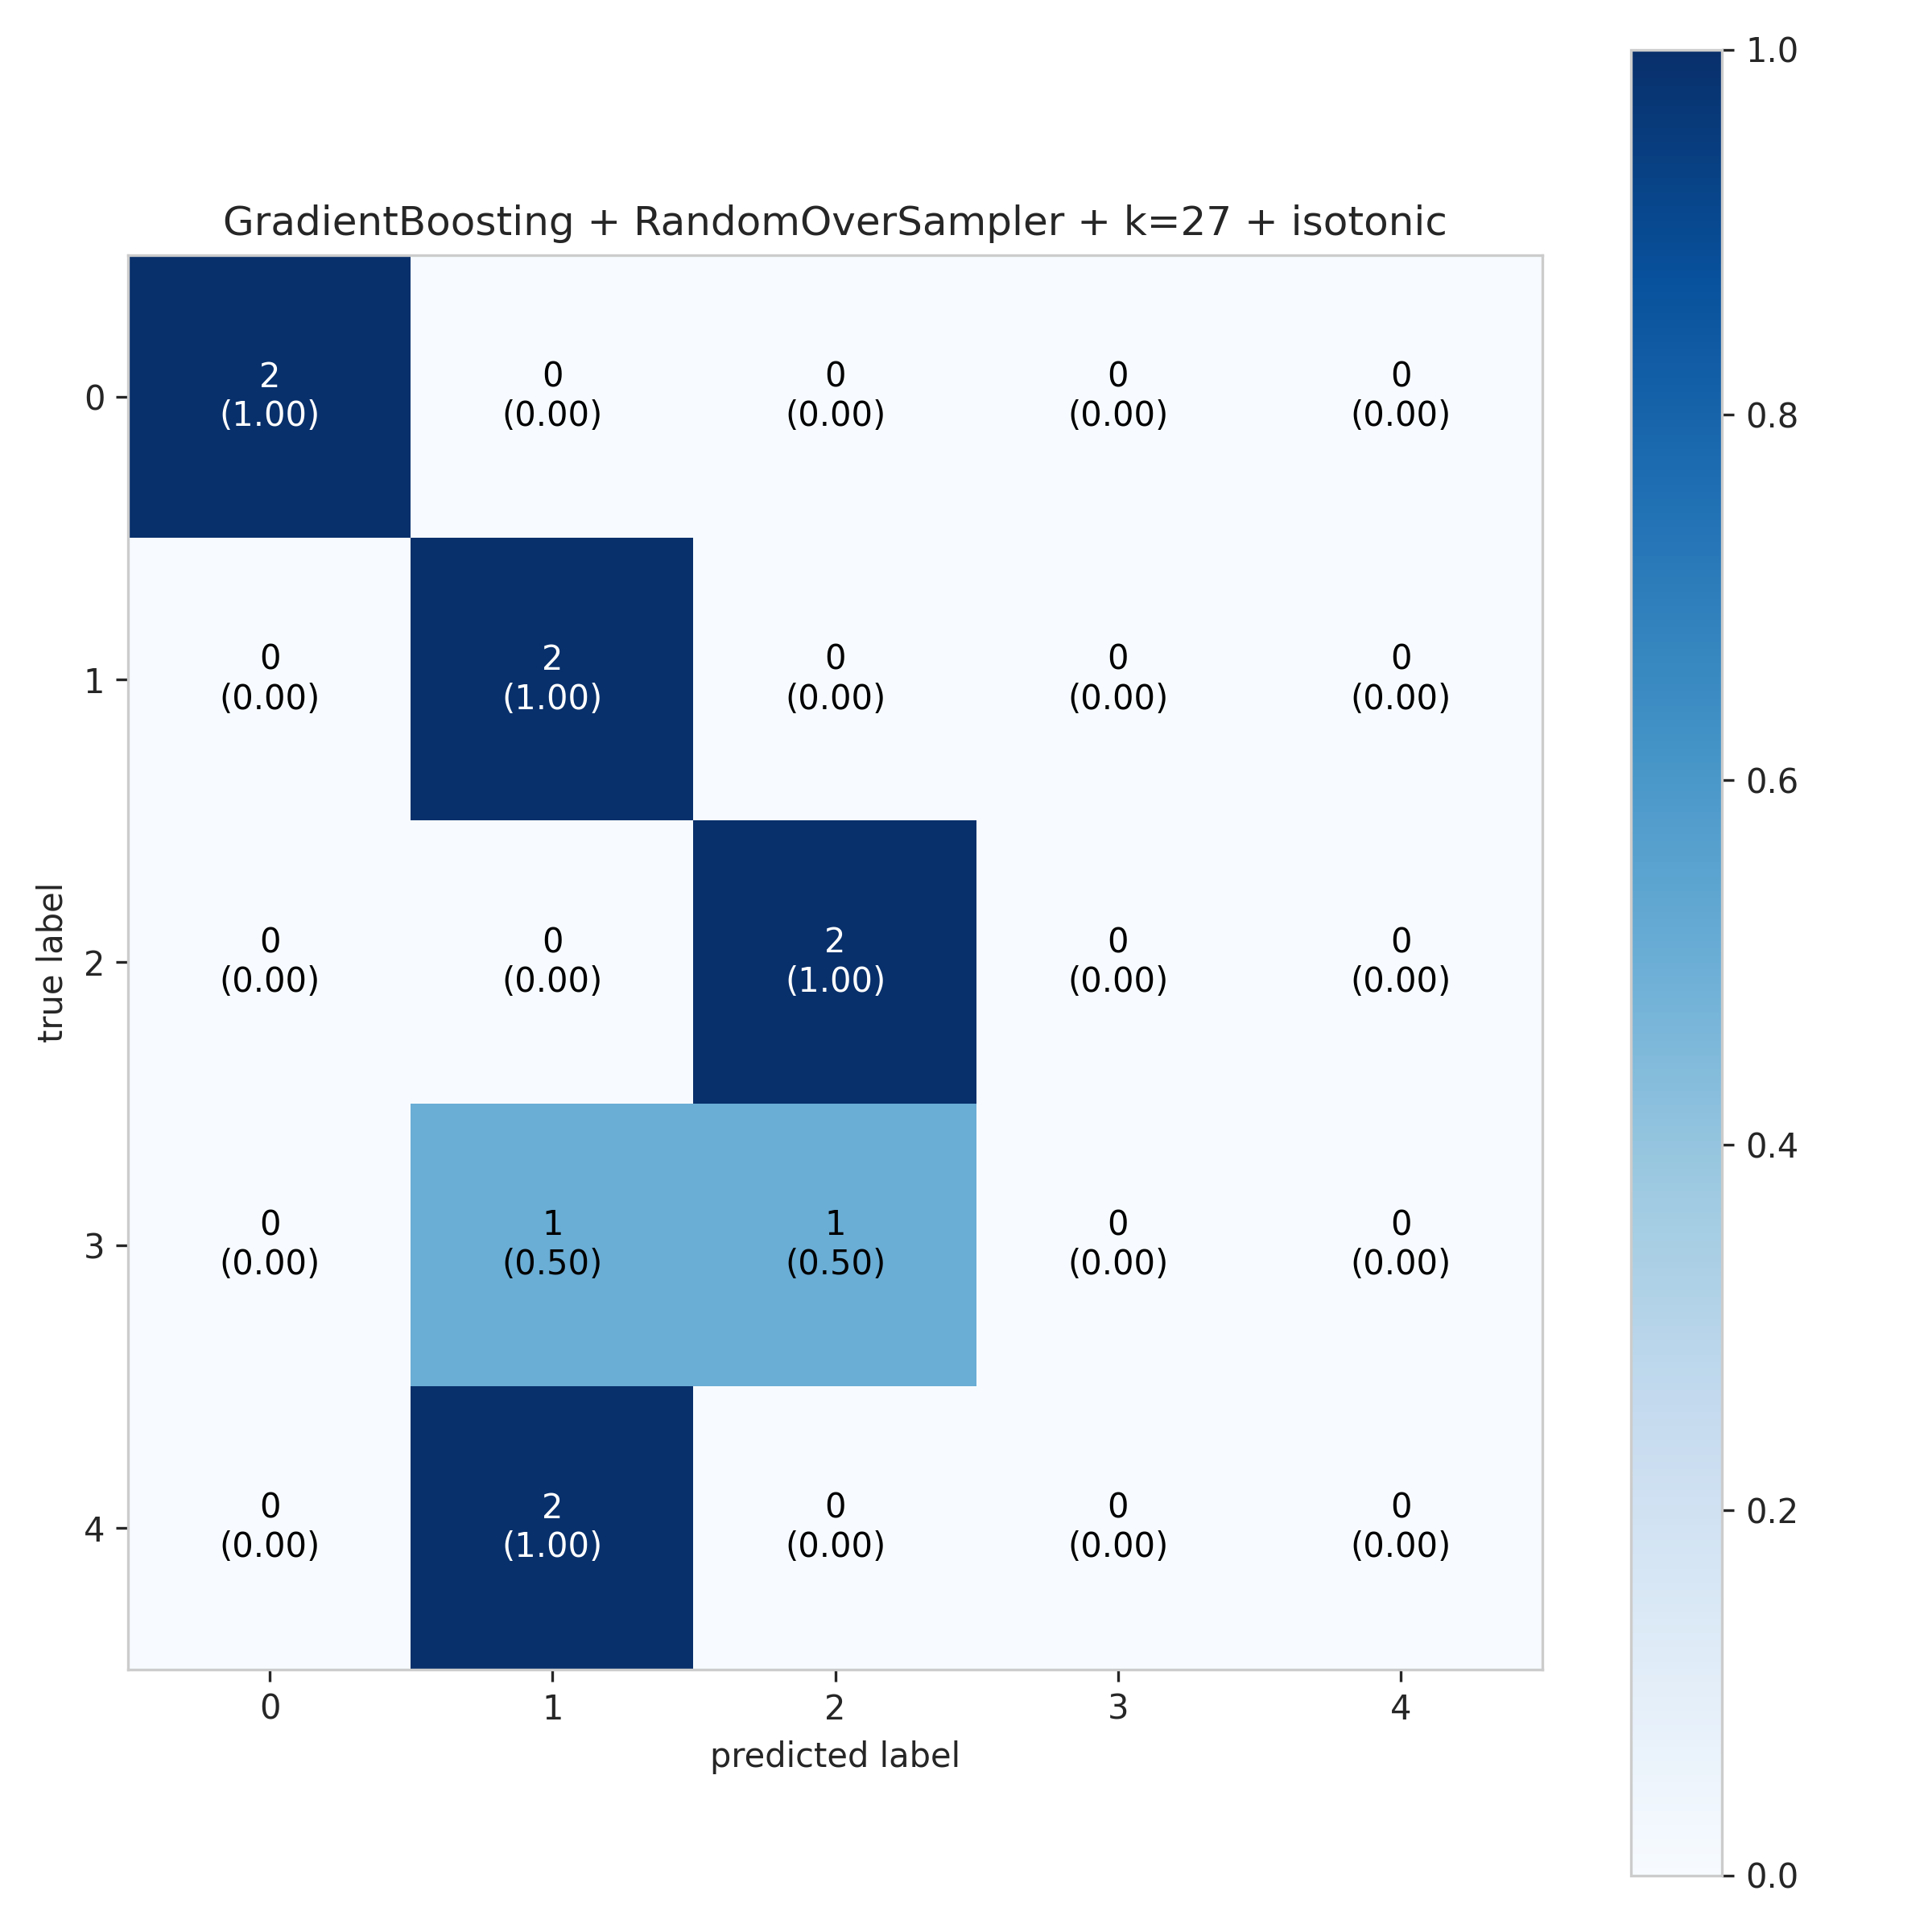
\includegraphics[width=\textwidth]{2005_cm.png}
    \caption{Gradient Boosting modeline ait karmaşıklık matrisi}
    \label{fig:resim2}
\end{minipage}
\end{figure}

\newpage

\subsection{2006 yılına ait model sonuçları}
2006 yılı için en iyi performansı \%60 sınama doğruluğu,  \%52.66 F1 skoru, \%53.33 kesinlik skoru ve \%53.33 duyarlılık skoru ile Logistic Regression modeli vermiştir.

\begin{figure}[ht]
\centering
\begin{minipage}[b]{0.7\textwidth}
    \centering
    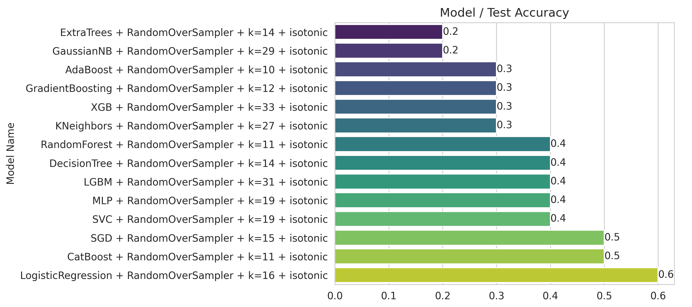
\includegraphics[width=\textwidth]{2006.png}
    \caption{2006 yılına ait model test doğrulukları.}
    \label{fig:resim1}
\end{minipage}
\hfill
\begin{minipage}[b]{0.6\textwidth}
    \centering
    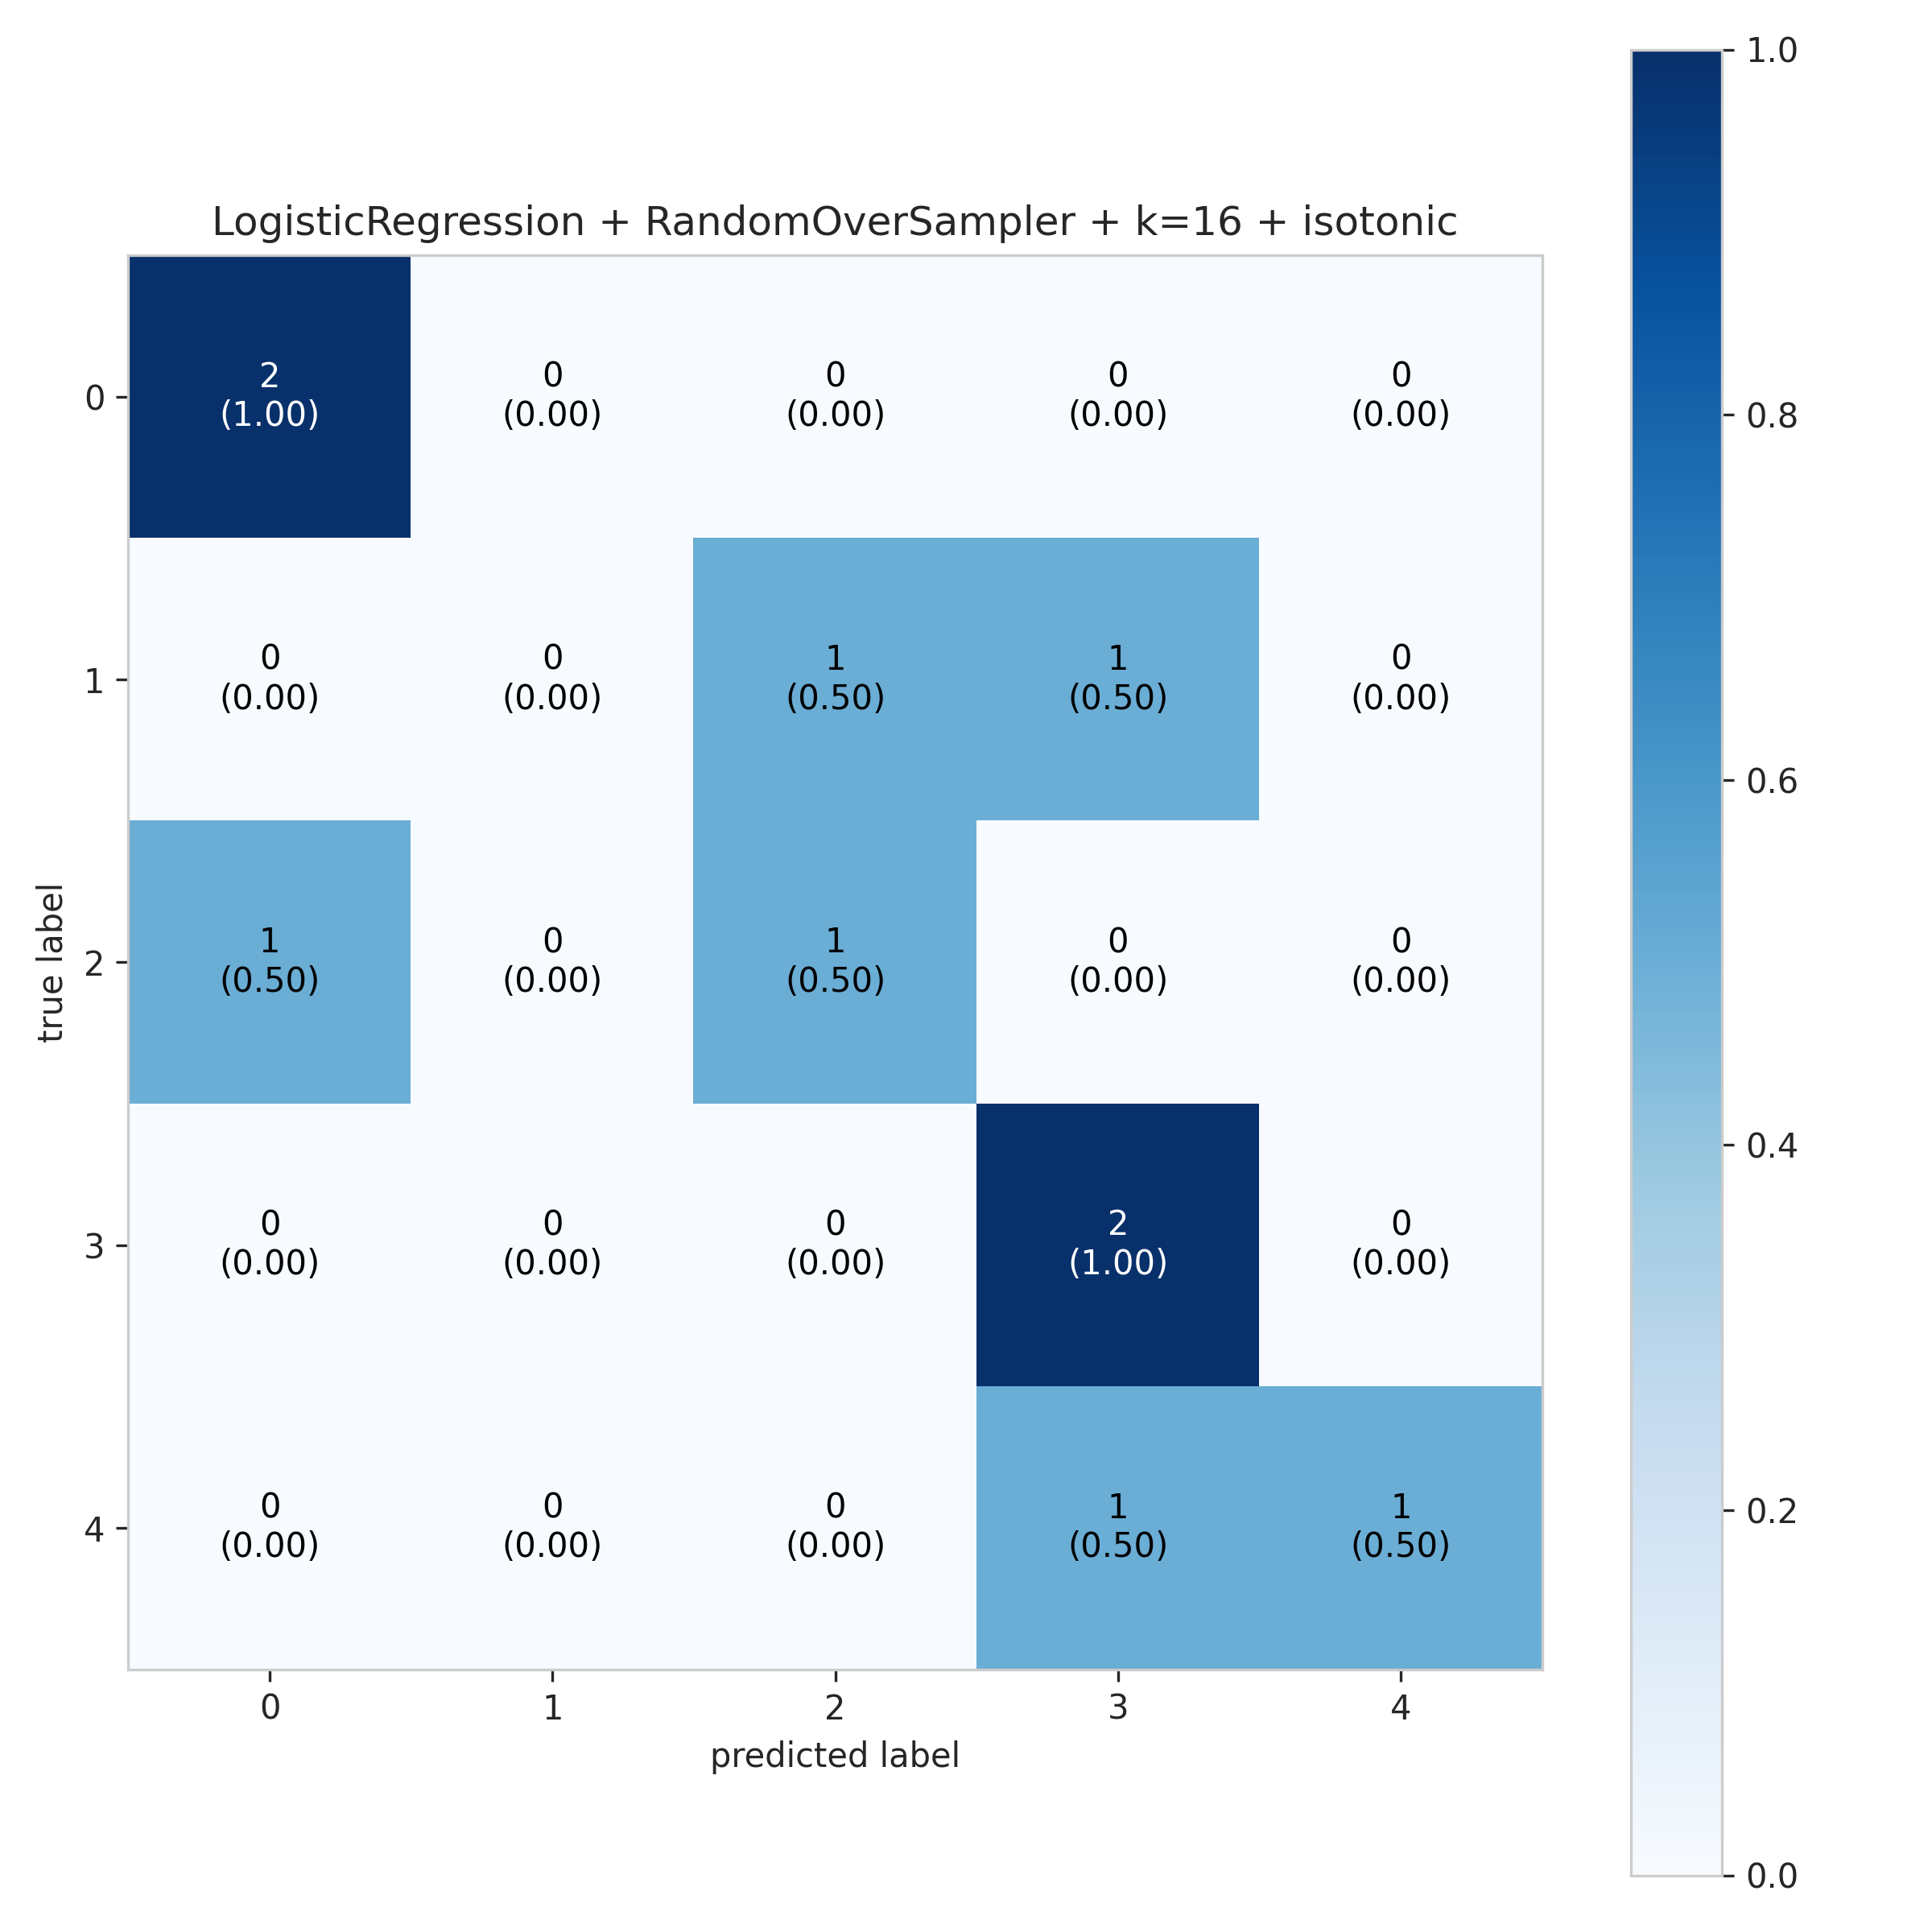
\includegraphics[width=\textwidth]{2006_cm.png}
    \caption{Logistic Regression modeline ait karmaşıklık matrisi}
    \label{fig:resim2}
\end{minipage}
\end{figure}
\newpage

\subsection{2007 yılına ait model sonuçları}
2007 yılı için en iyi performansı \%60 sınama doğruluğu,  \%61.33 F1 skoru, \%76.66 kesinlik skoru ve \%76.66 duyarlılık skoru ile MLP modeli vermiştir.

\begin{figure}[ht]
\centering
\begin{minipage}[b]{0.6\textwidth}
    \centering
    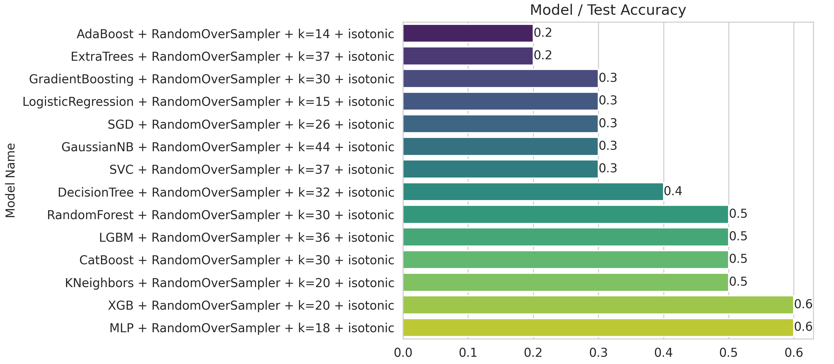
\includegraphics[width=\textwidth]{2007.png}
    \caption{2007 yılına ait model test doğrulukları.}
    \label{fig:resim1}
\end{minipage}
\hfill
\begin{minipage}[b]{0.6\textwidth}
    \centering
    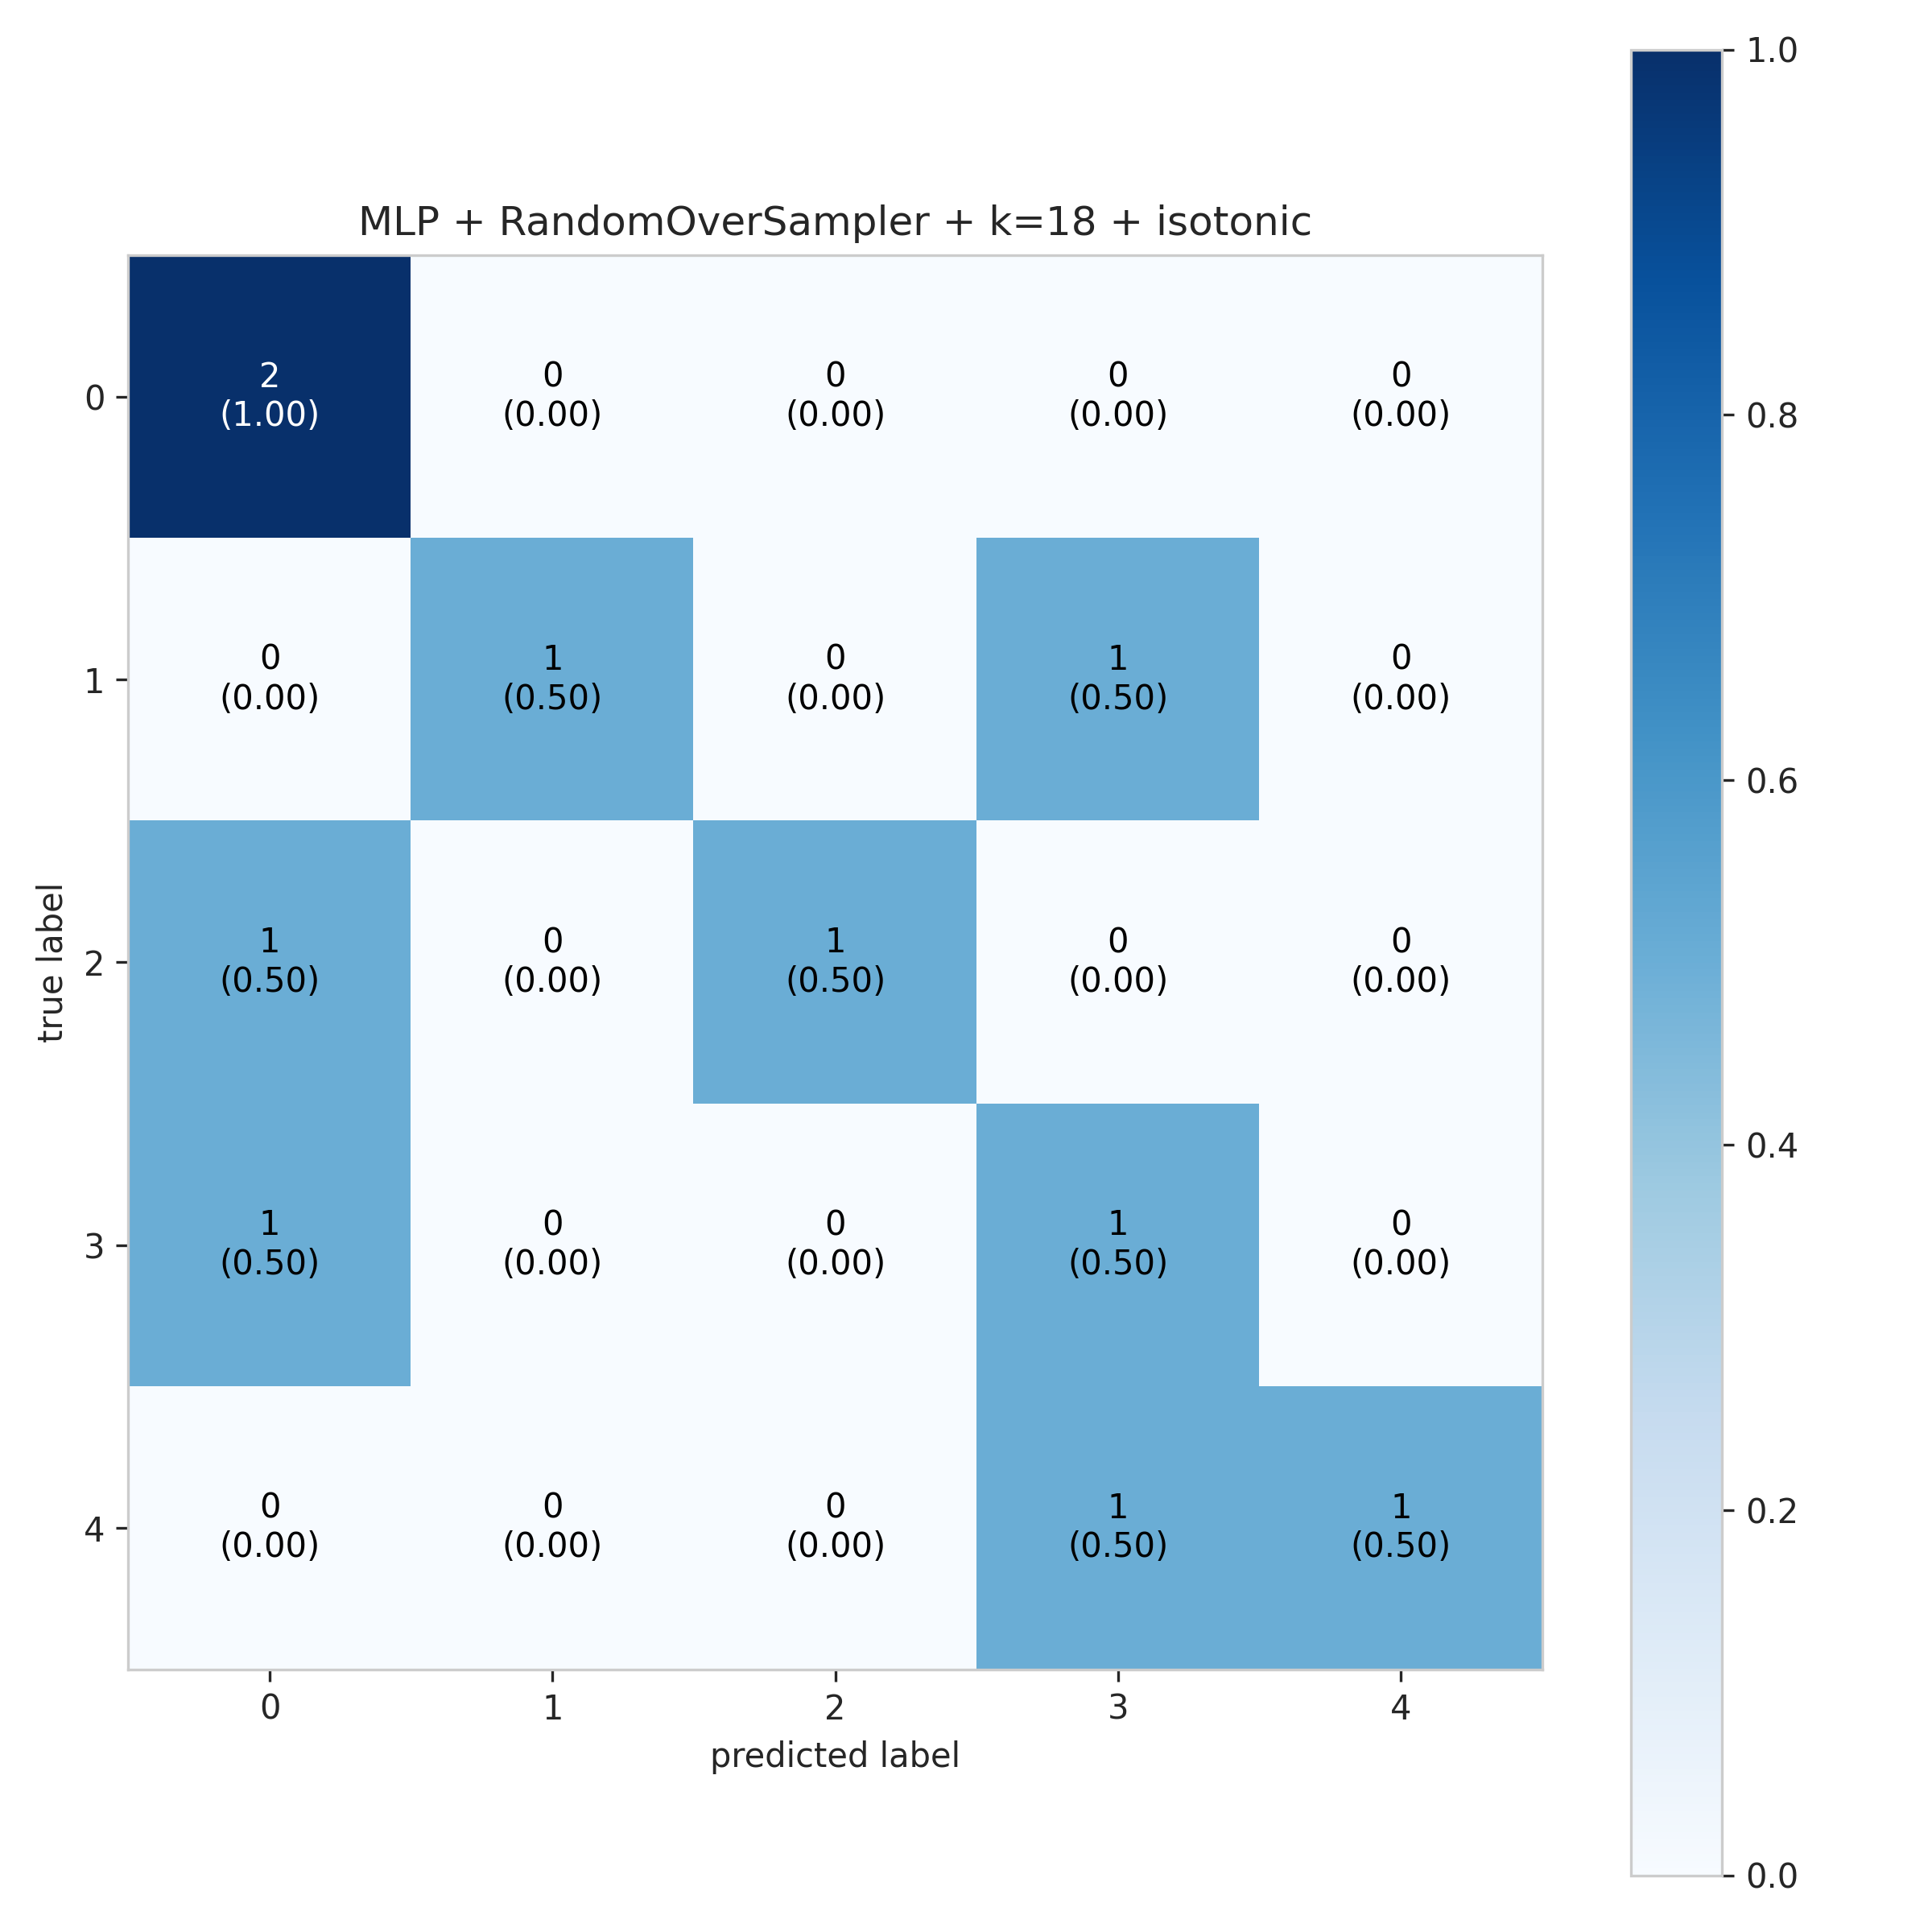
\includegraphics[width=\textwidth]{2007_cm.png}
    \caption{MLP modeline ait karmaşıklık matrisi}
    \label{fig:resim2}
\end{minipage}
\end{figure}
\newpage

\subsection{2008 yılına ait model sonuçları}
2008 yılı için en iyi performansı \%50 sınama doğruluğu,  \%44.76 F1 skoru, \%48 kesinlik skoru ve \%48 duyarlılık skoru ile XGB modeli vermiştir.

\begin{figure}[ht]
\centering
\begin{minipage}[b]{0.6\textwidth}
    \centering
    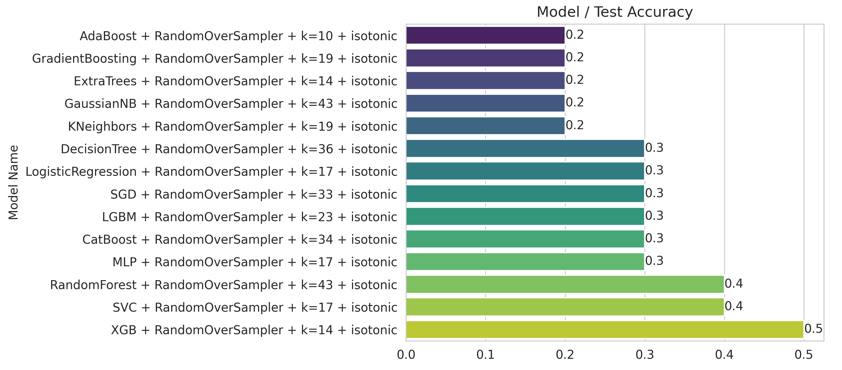
\includegraphics[width=\textwidth]{2008.png}
    \caption{2008 yılına ait model test doğrulukları.}
    \label{fig:resim1}
\end{minipage}
\hfill
\begin{minipage}[b]{0.6\textwidth}
    \centering
    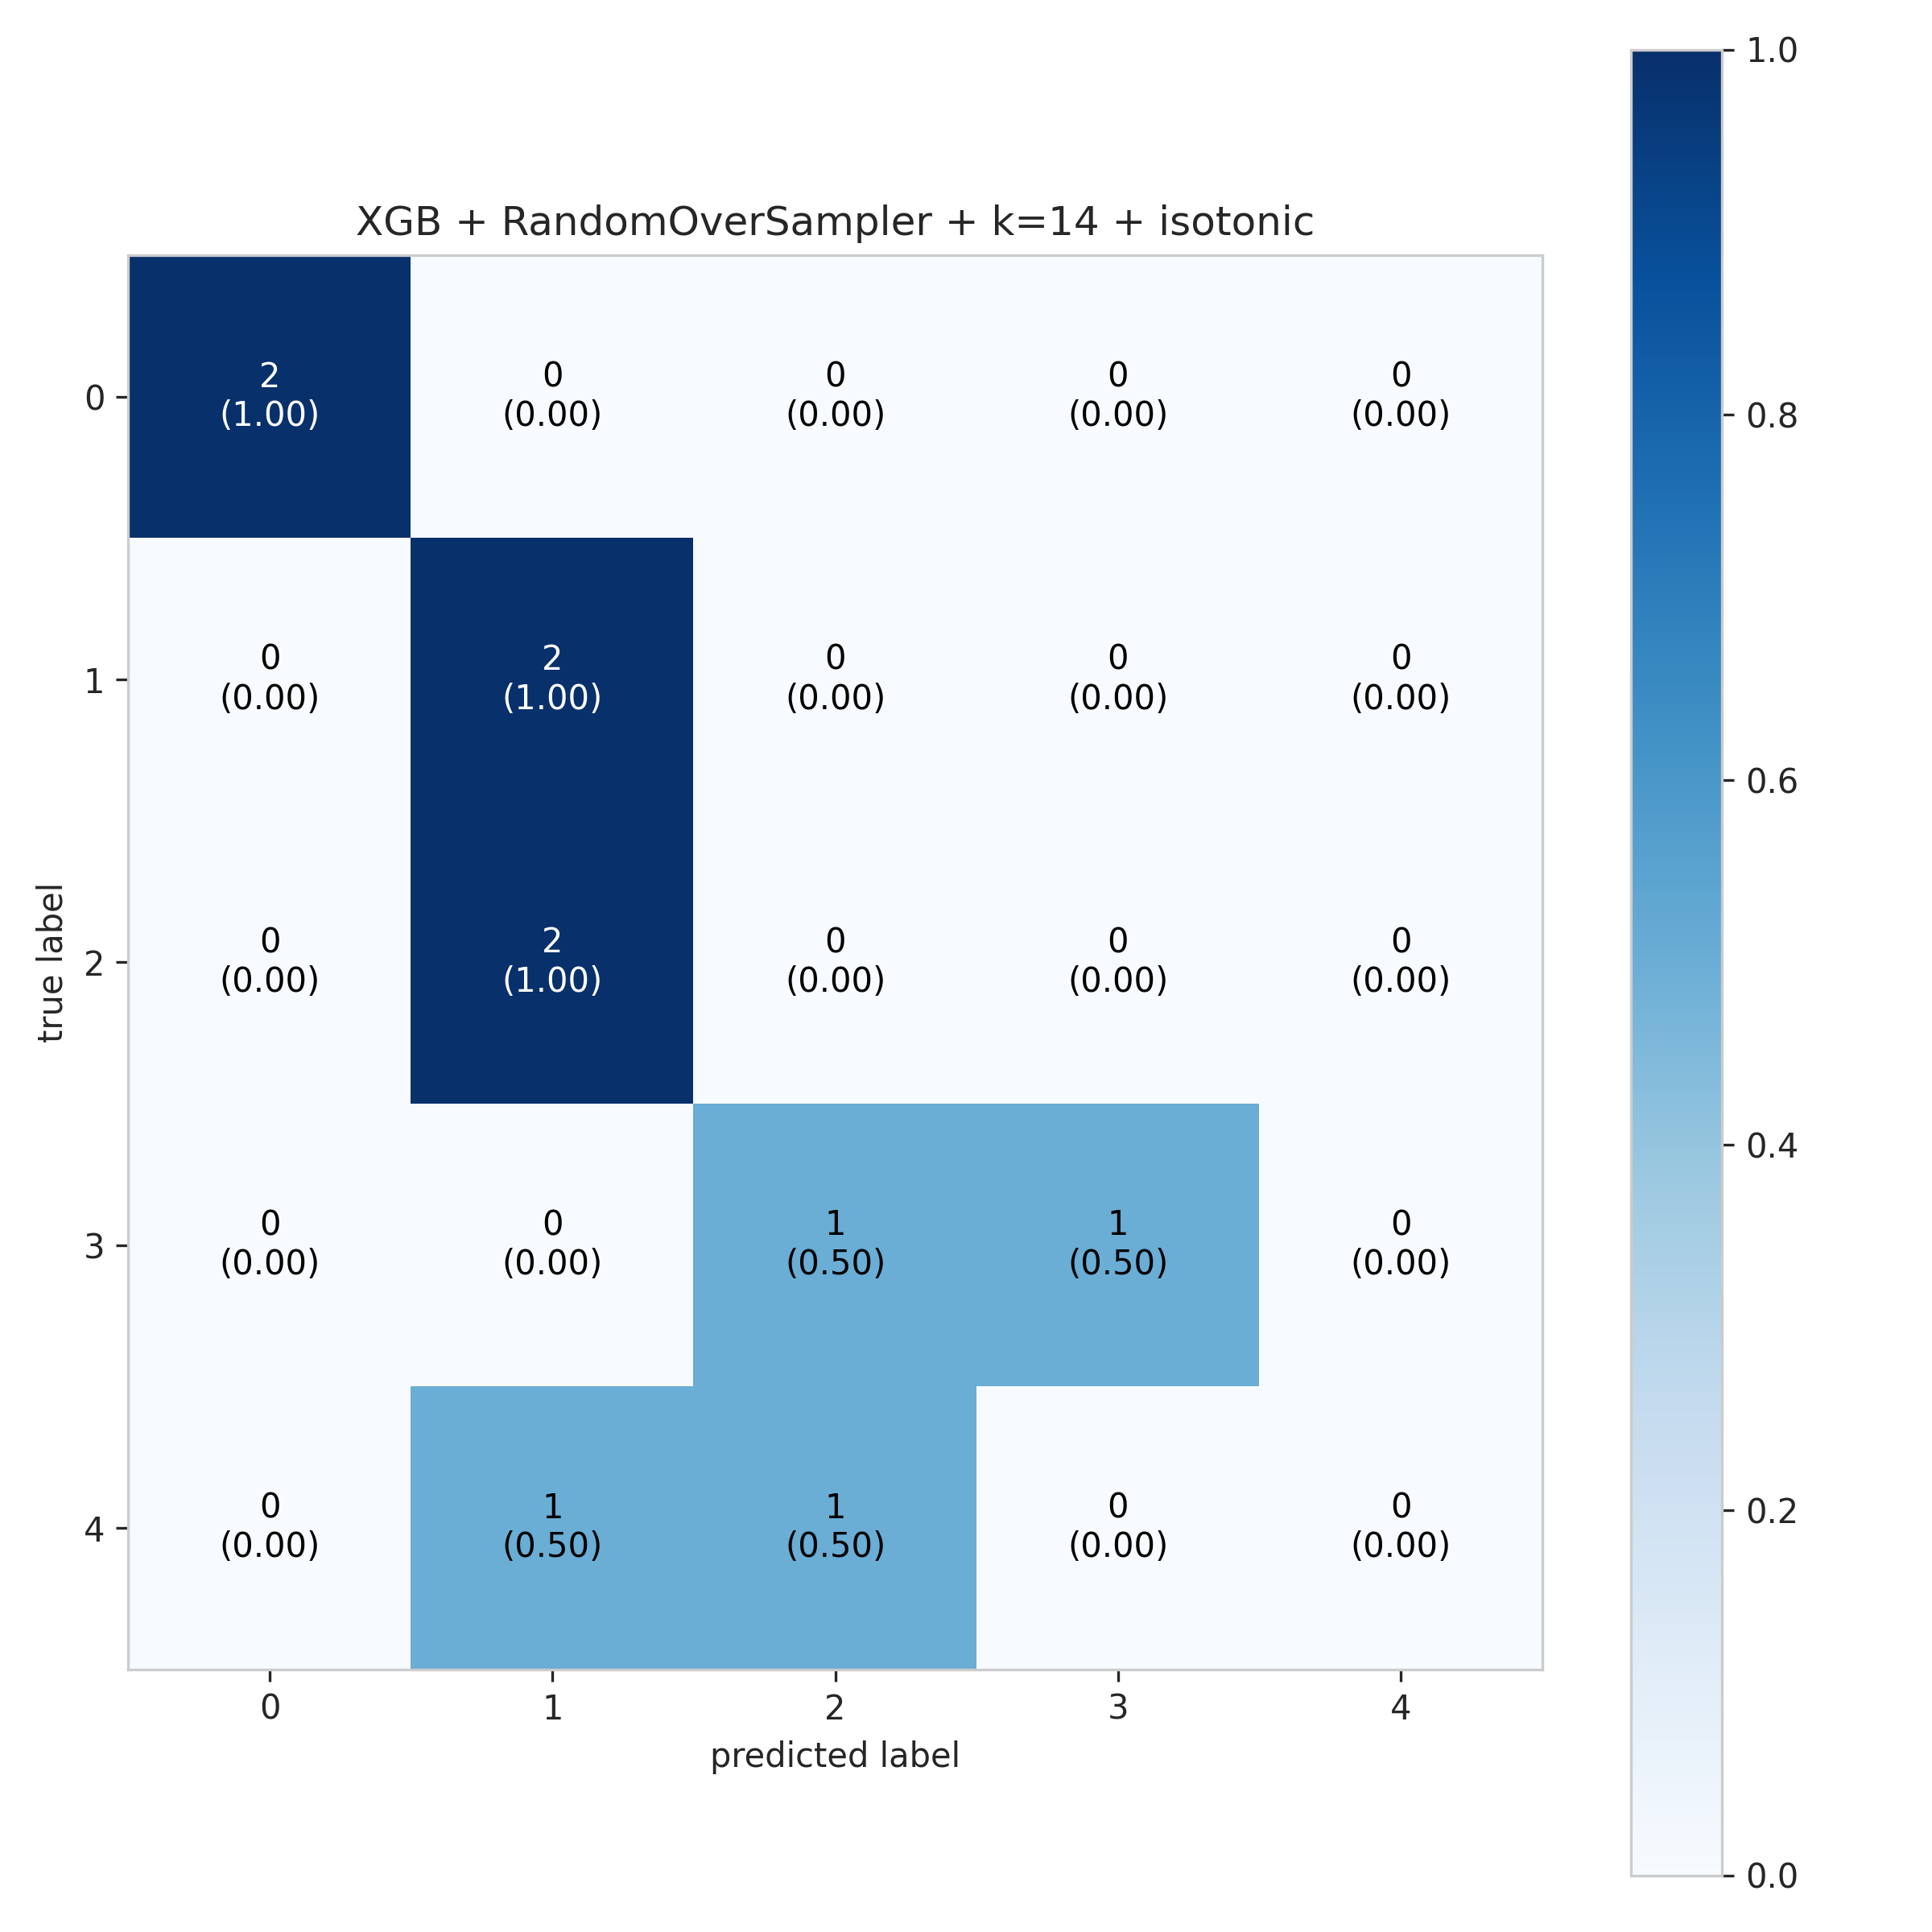
\includegraphics[width=\textwidth]{2008_cm.png}
    \caption{XGB modeline ait karmaşıklık matrisi}
    \label{fig:resim2}
\end{minipage}
\end{figure}

\newpage

\subsection{2009 yılına ait model sonuçları}
2009 yılı için en iyi performansı \%60 sınama doğruluğu,  \%58.09 F1 skoru, \%68 kesinlik skoru ve \%68 duyarlılık skoru ile Decision Tree modeli vermiştir.

\begin{figure}[ht]
\centering
\begin{minipage}[b]{0.6\textwidth}
    \centering
    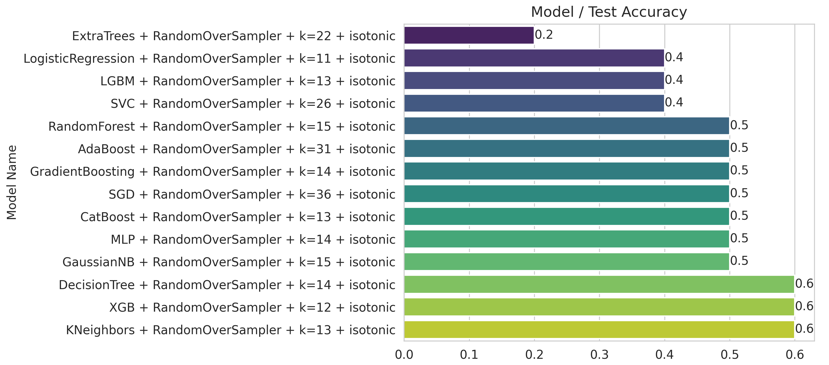
\includegraphics[width=\textwidth]{2009.png}
    \caption{2009 yılına ait model test doğrulukları.}
    \label{fig:resim1}
\end{minipage}
\hfill
\begin{minipage}[b]{0.6\textwidth}
    \centering
    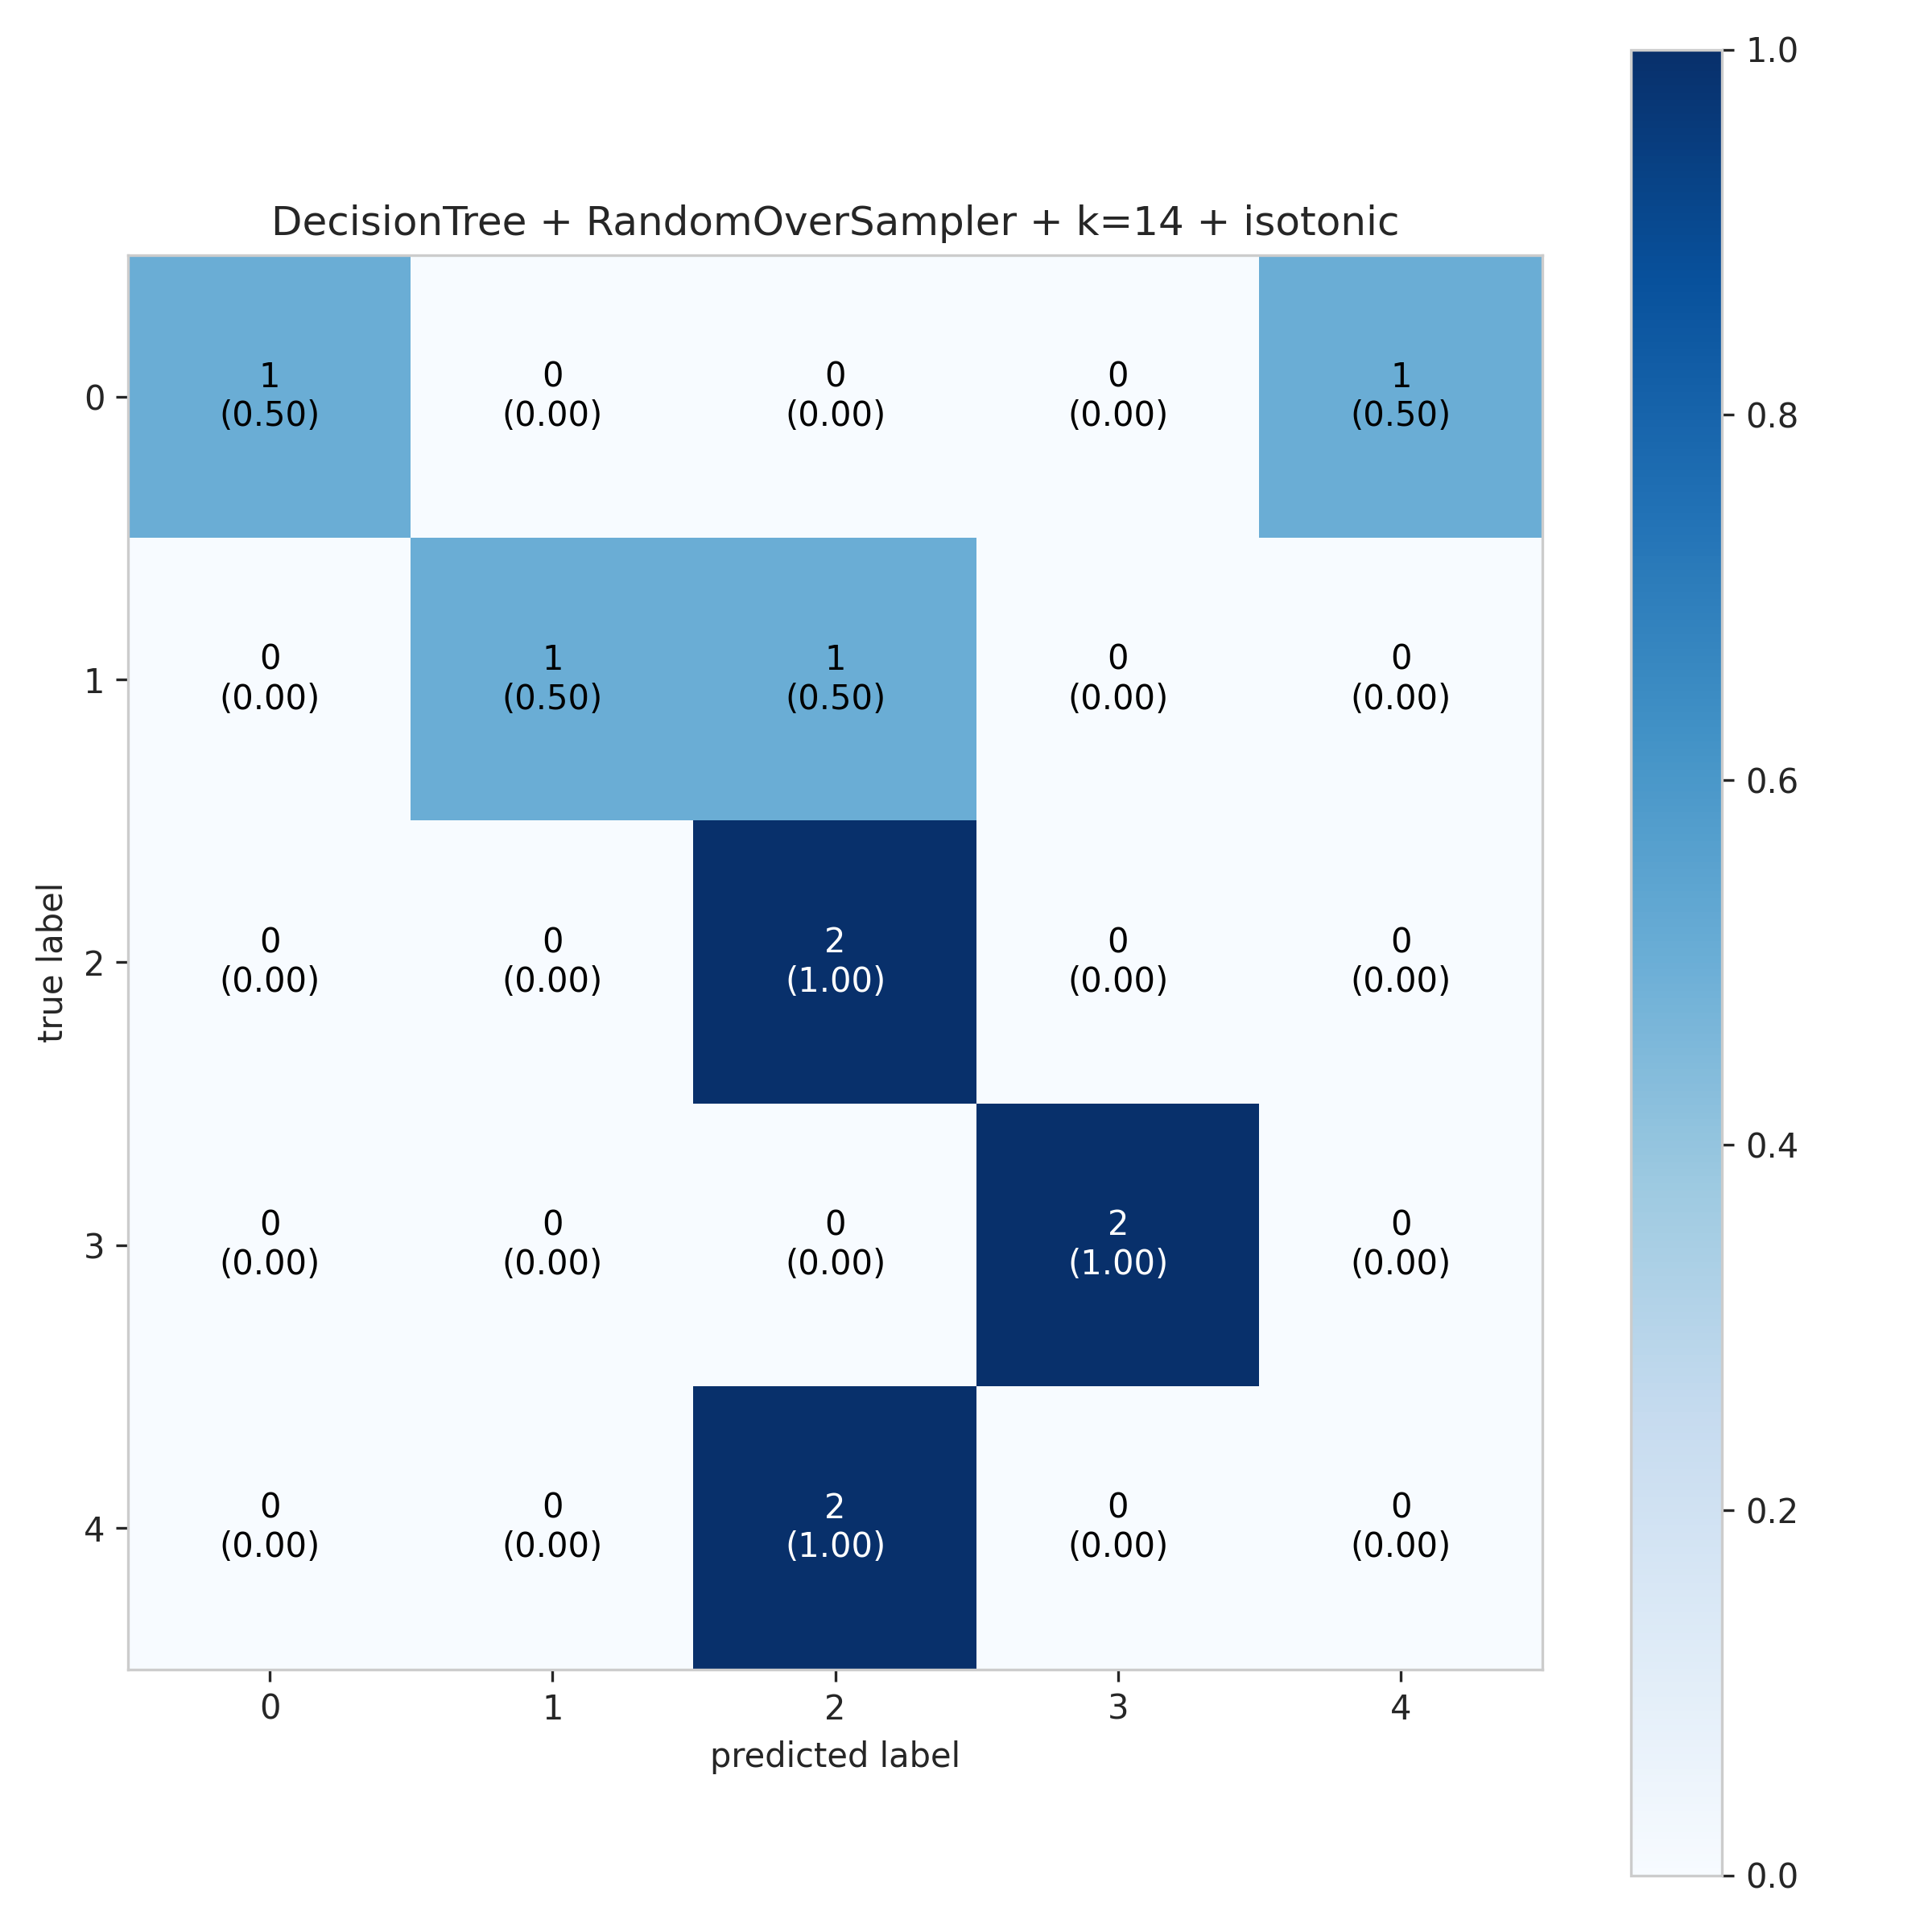
\includegraphics[width=\textwidth]{2009_cm.png}
    \caption{Decision Tree modeline ait karmaşıklık matrisi}
    \label{fig:resim2}
\end{minipage}
\end{figure}

\newpage

\subsection{2010 yılına ait model sonuçları}
2010 yılı için en iyi performansı \%60 sınama doğruluğu,  \%61.42 F1 skoru, \%78 kesinlik skoru ve \%78 duyarlılık skoru ile Logistic Regression modeli vermiştir.

\begin{figure}[ht]
\centering
\begin{minipage}[b]{0.6\textwidth}
    \centering
    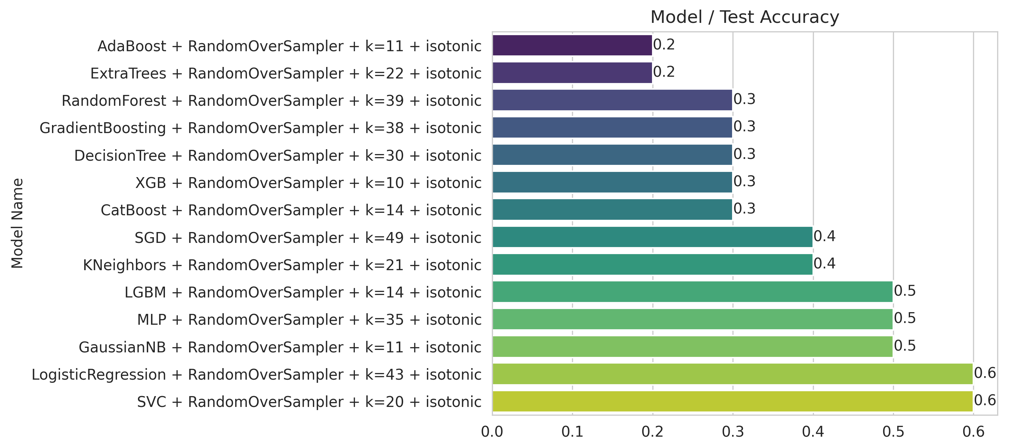
\includegraphics[width=\textwidth]{2010.png}
    \caption{2010 yılına ait model test doğrulukları.}
    \label{fig:resim1}
\end{minipage}
\hfill
\begin{minipage}[b]{0.6\textwidth}
    \centering
    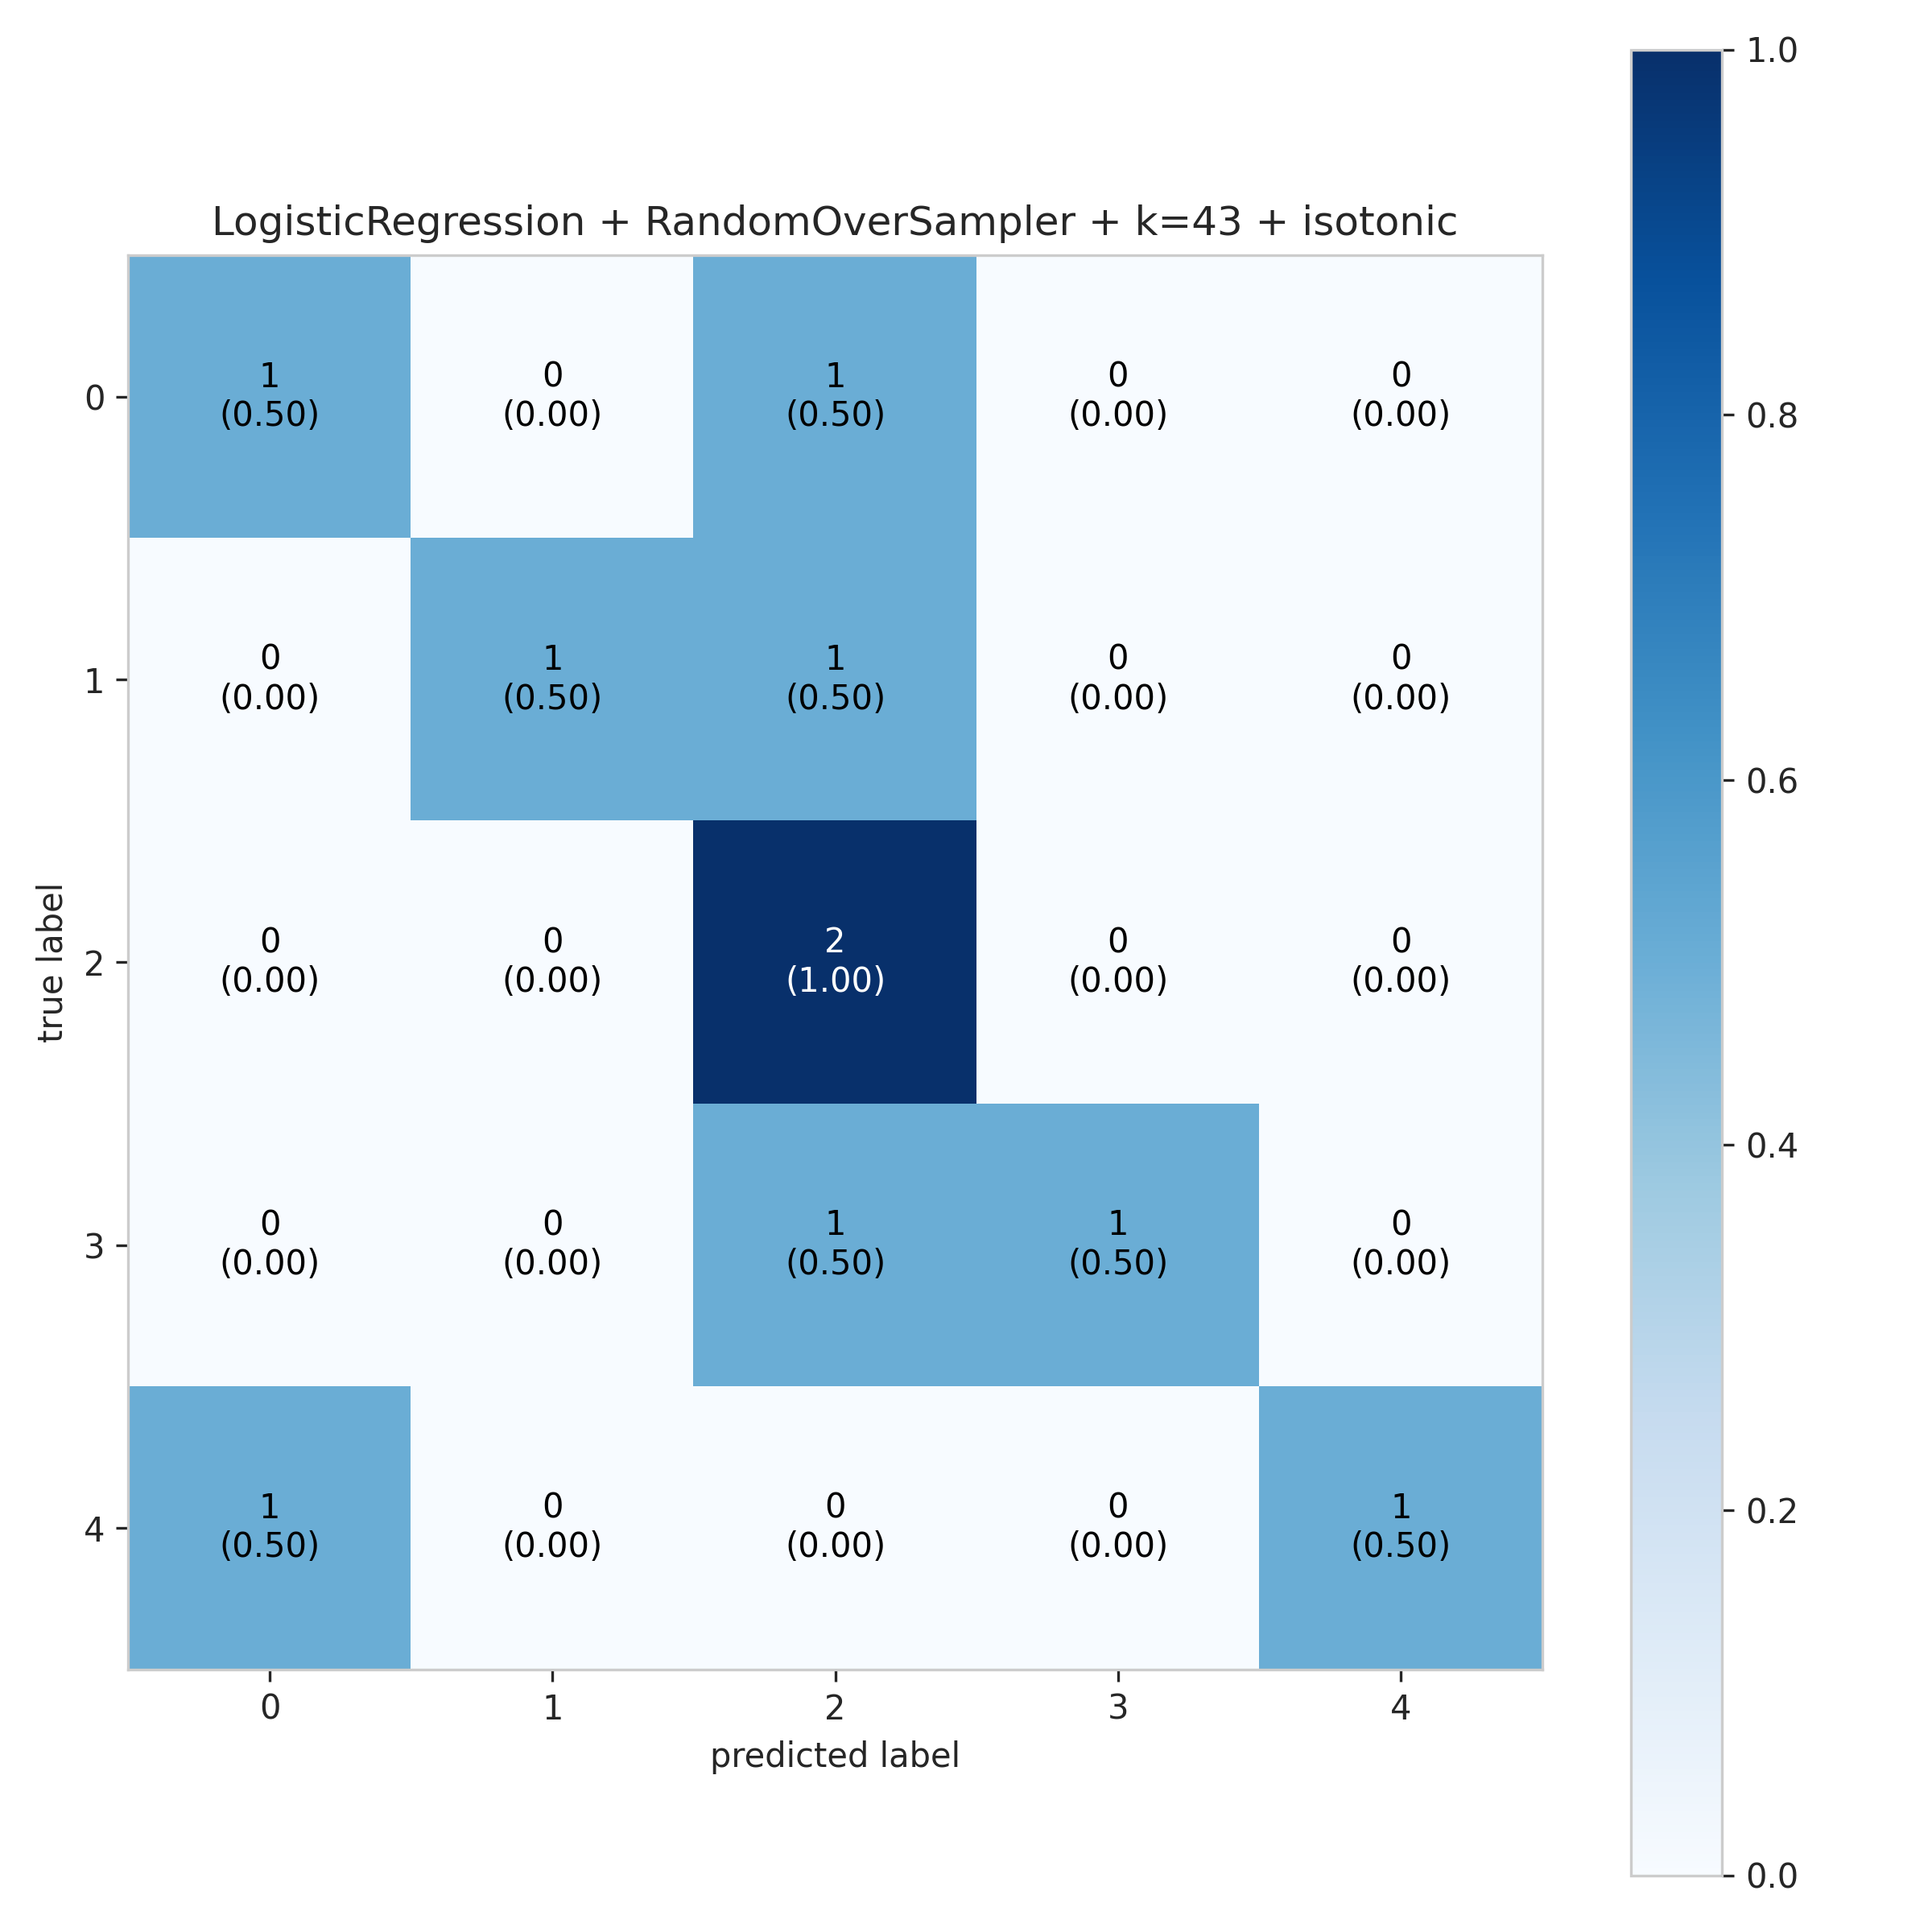
\includegraphics[width=\textwidth]{2010_cm.png}
    \caption{Logistic Regression modeline ait karmaşıklık matrisi}
    \label{fig:resim2}
\end{minipage}
\end{figure}

\newpage

\subsection{2011 yılına ait model sonuçları}
2011 yılı için en iyi performansı \%40 sınama doğruluğu,  \%32 F1 skoru, \%26.66 kesinlik skoru ve \%26.66 duyarlılık skoru ile Logistic Regression modeli vermiştir.

\begin{figure}[ht]
\centering
\begin{minipage}[b]{0.6\textwidth}
    \centering
    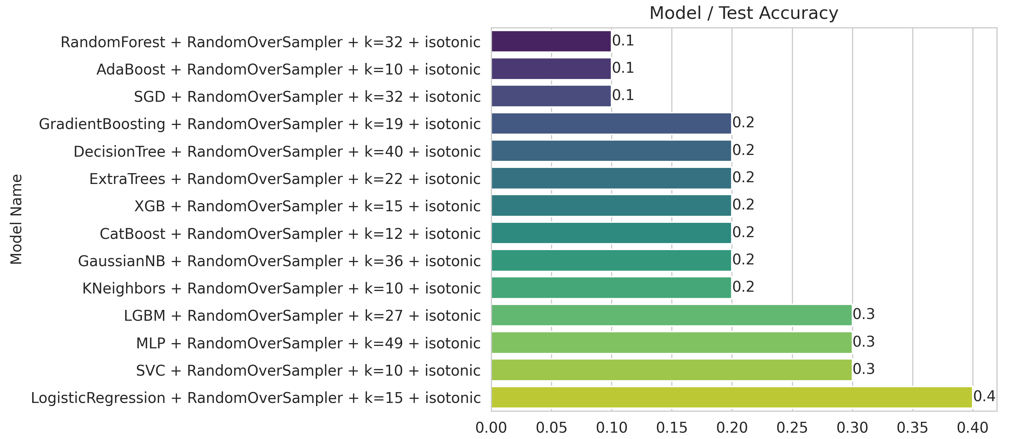
\includegraphics[width=\textwidth]{2011.png}
    \caption{2011 yılına ait model test doğrulukları.}
    \label{fig:resim1}
\end{minipage}
\hfill
\begin{minipage}[b]{0.6\textwidth}
    \centering
    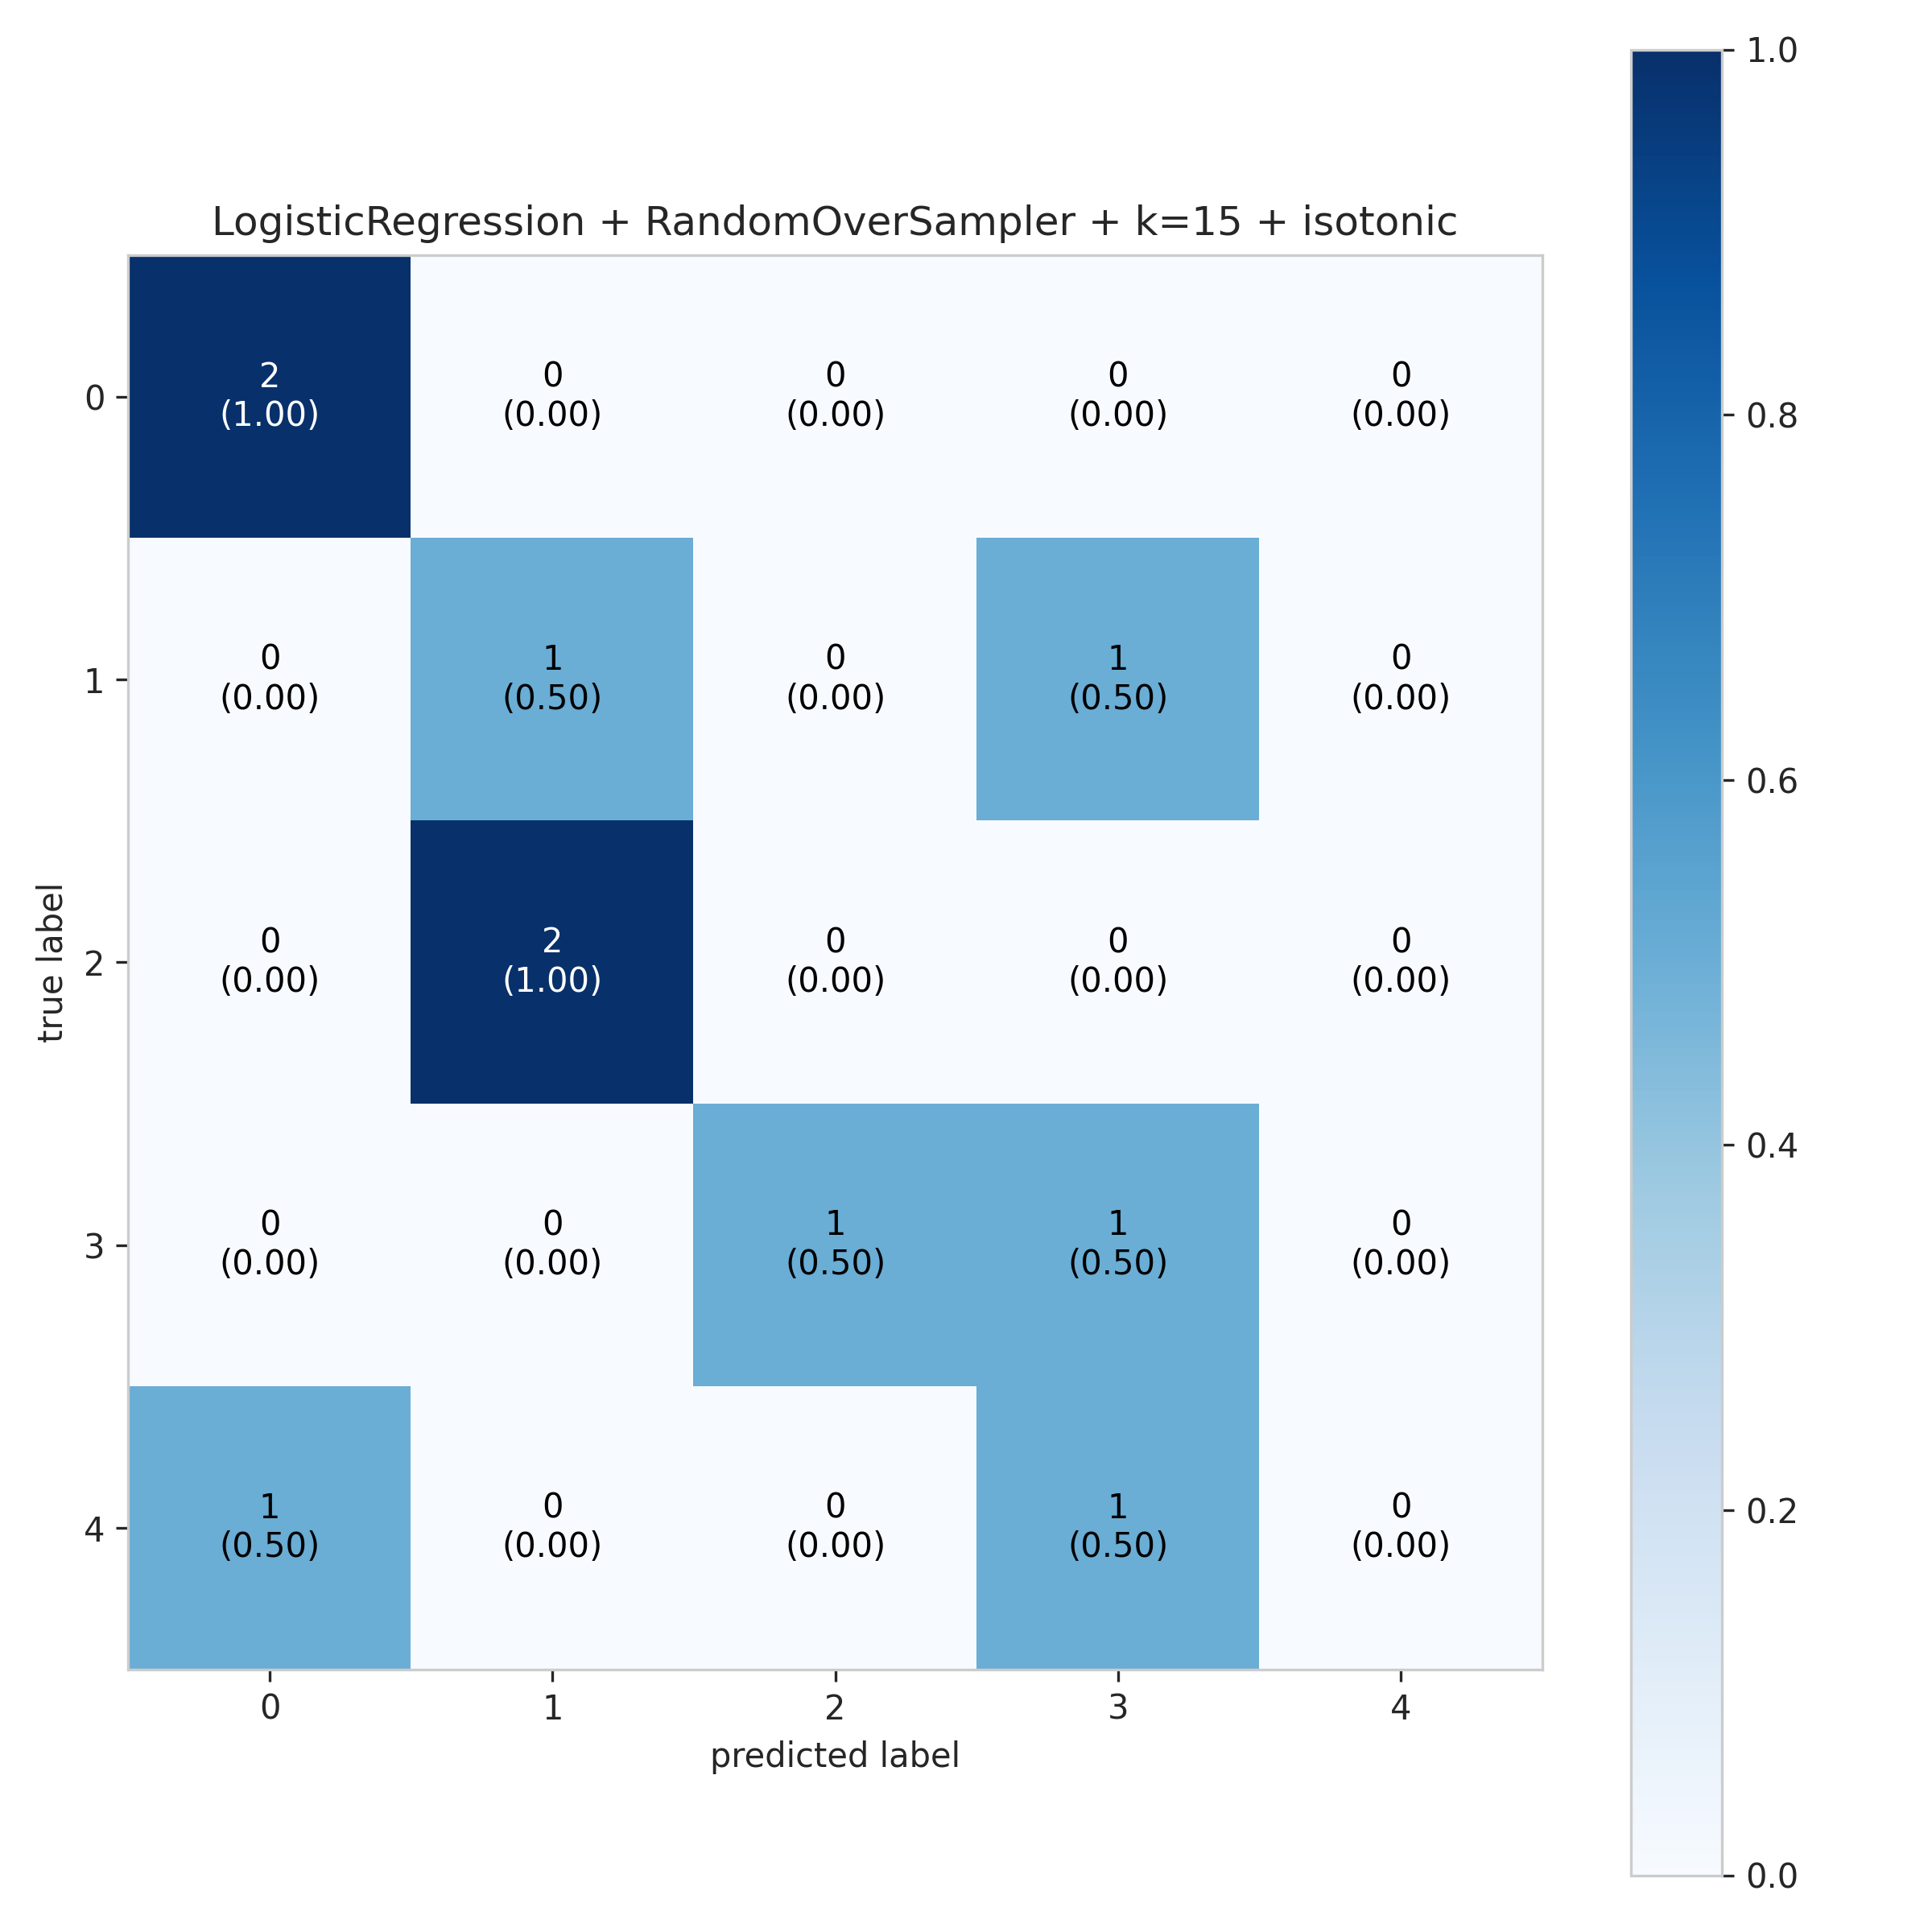
\includegraphics[width=\textwidth]{2011_cm.png}
    \caption{Logistic Regression modeline ait karmaşıklık matrisi}
    \label{fig:resim2}
\end{minipage}
\end{figure}

\newpage

\subsection{2012 yılına ait model sonuçları}
2012 yılı için en iyi performansı \%33.33 sınama doğruluğu,  \%34.66 F1 skoru, \%52.38 kesinlik skoru ve \%52.38 duyarlılık skoru ile MLP modeli vermiştir.

\begin{figure}[ht]
\centering
\begin{minipage}[b]{0.6\textwidth}
    \centering
    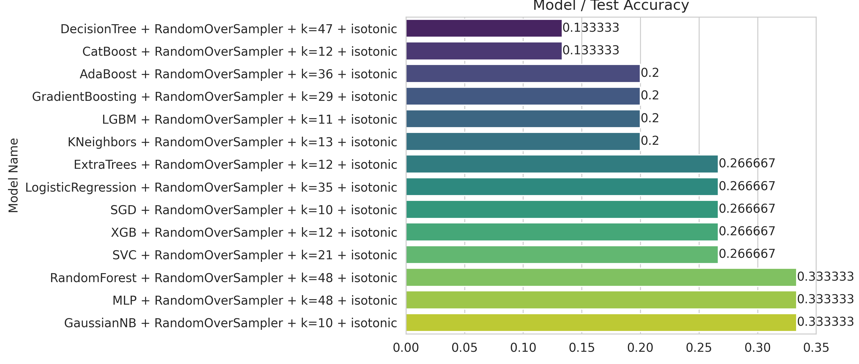
\includegraphics[width=\textwidth]{2012.png}
    \caption{2012 yılına ait model test doğrulukları.}
    \label{fig:resim1}
\end{minipage}
\hfill
\begin{minipage}[b]{0.6\textwidth}
    \centering
    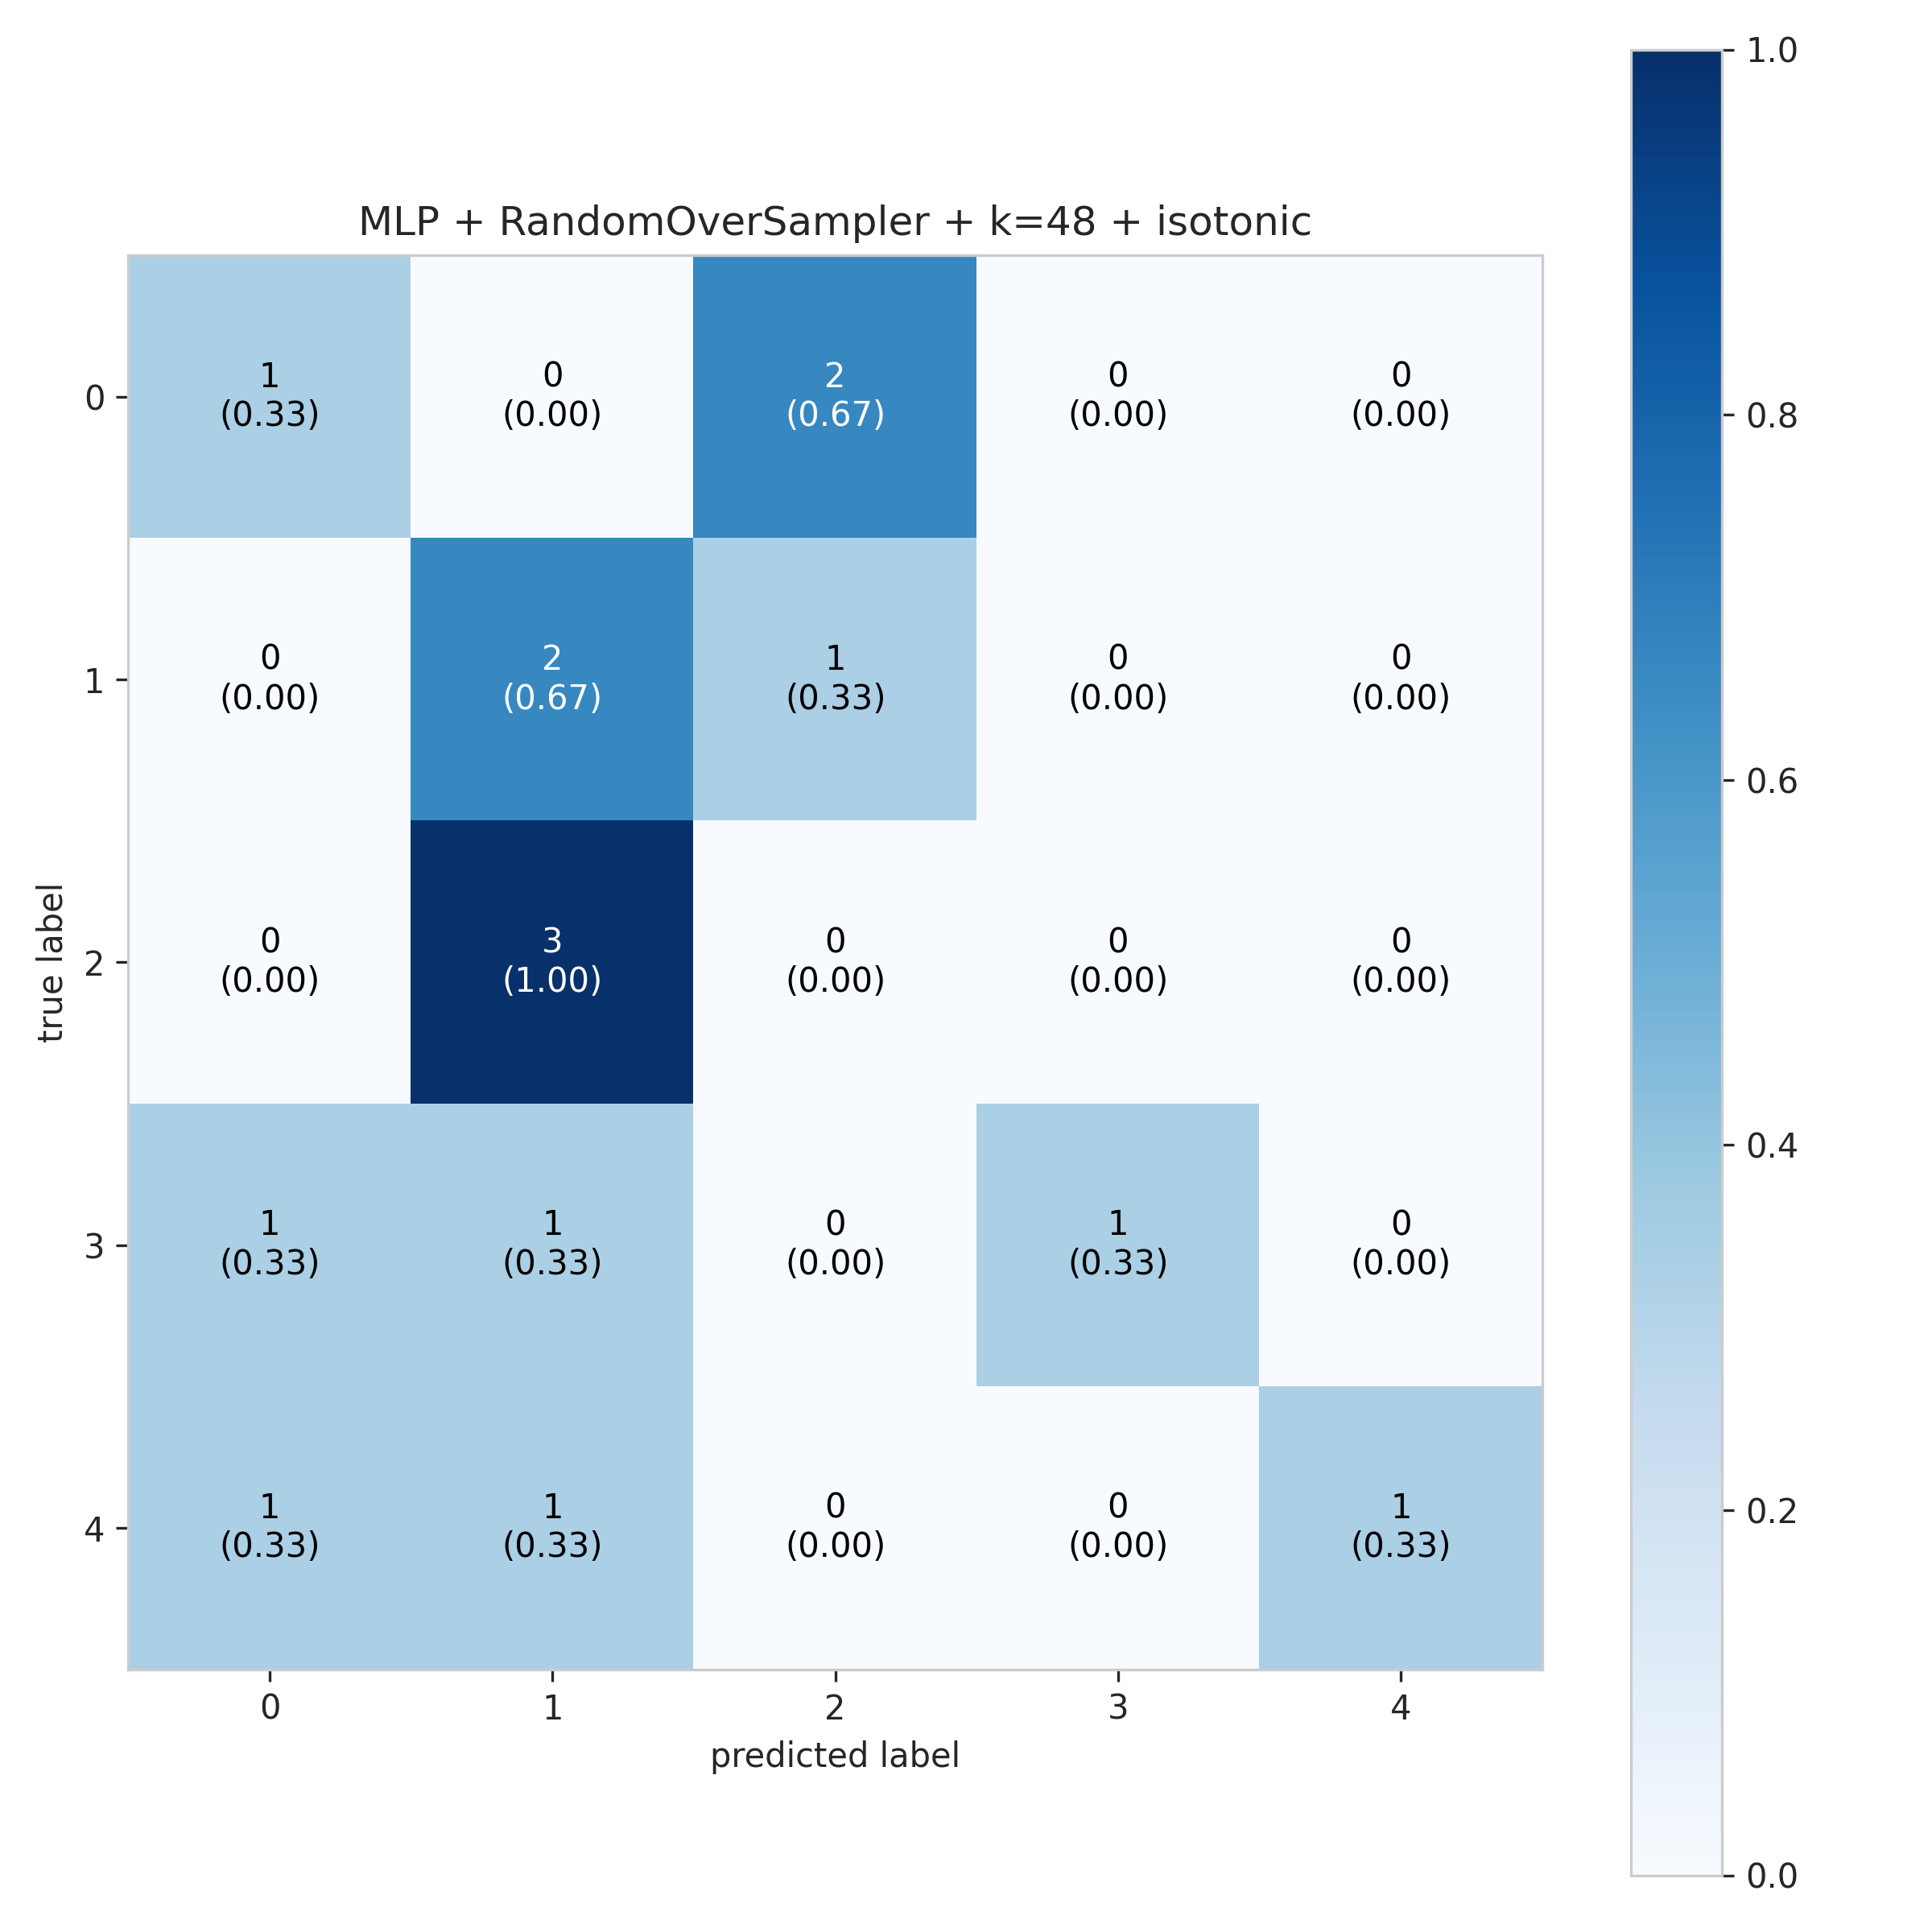
\includegraphics[width=\textwidth]{2012_cm.png}
    \caption{MLP modeline ait karmaşıklık matrisi}
    \label{fig:resim2}
\end{minipage}
\end{figure}

\newpage

\subsection{2013 yılına ait model sonuçları}
2013 yılı için en iyi performansı \%53.33 sınama doğruluğu,  \%49.57 F1 skoru, \%49 kesinlik skoru ve \%49 duyarlılık skoru ile SVC modeli vermiştir.

\begin{figure}[ht]
\centering
\begin{minipage}[b]{0.6\textwidth}
    \centering
    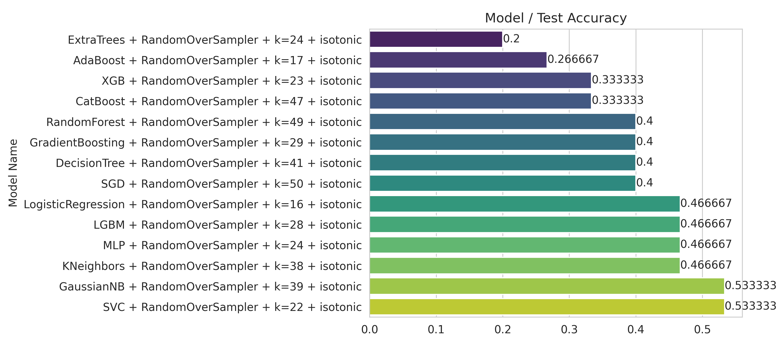
\includegraphics[width=\textwidth]{2013.png}
    \caption{2013 yılına ait model test doğrulukları.}
    \label{fig:resim1}
\end{minipage}
\hfill
\begin{minipage}[b]{0.6\textwidth}
    \centering
    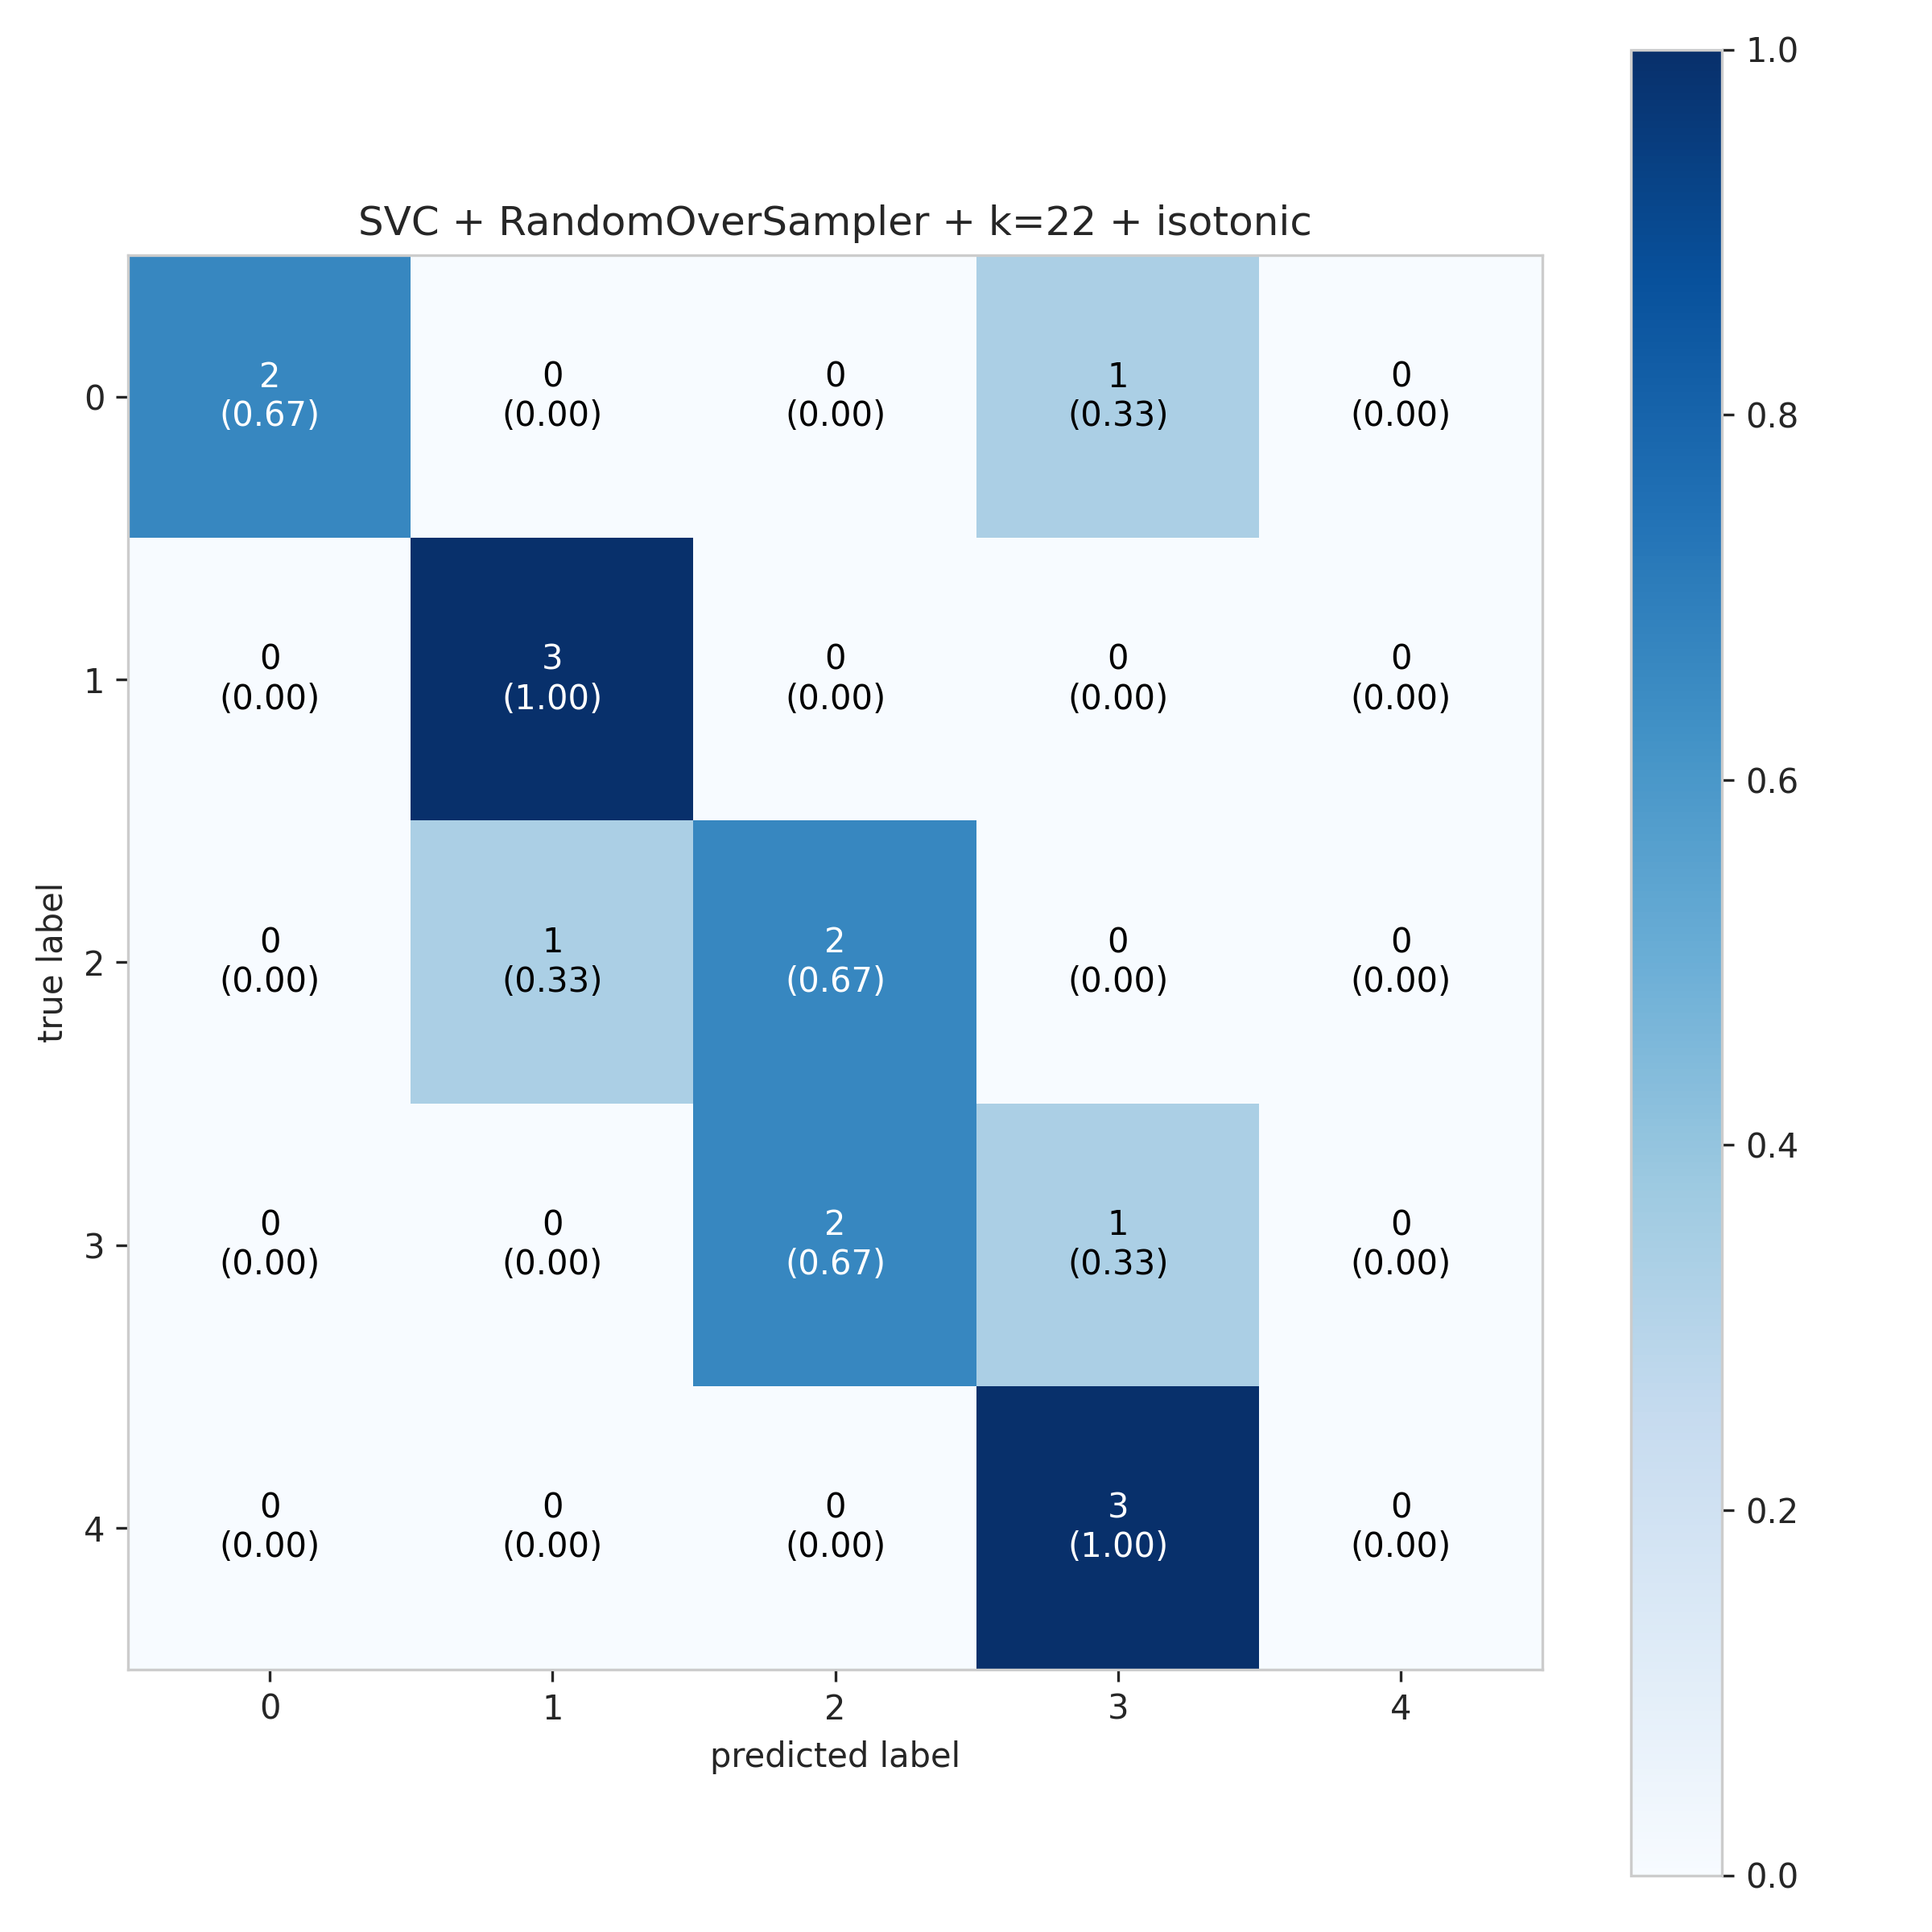
\includegraphics[width=\textwidth]{2013_cm.png}
    \caption{SVC modeline ait karmaşıklık matrisi}
    \label{fig:resim2}
\end{minipage}
\end{figure}

\newpage

\subsection{2014 yılına ait model sonuçları}
2014 yılı için en iyi performansı \%40 sınama doğruluğu,  \%38 F1 skoru, \%46.66 kesinlik skoru ve \%46.66 duyarlılık skoru ile Gaussian Naive Bayes modeli vermiştir.

\begin{figure}[ht]
\centering
\begin{minipage}[b]{0.6\textwidth}
    \centering
    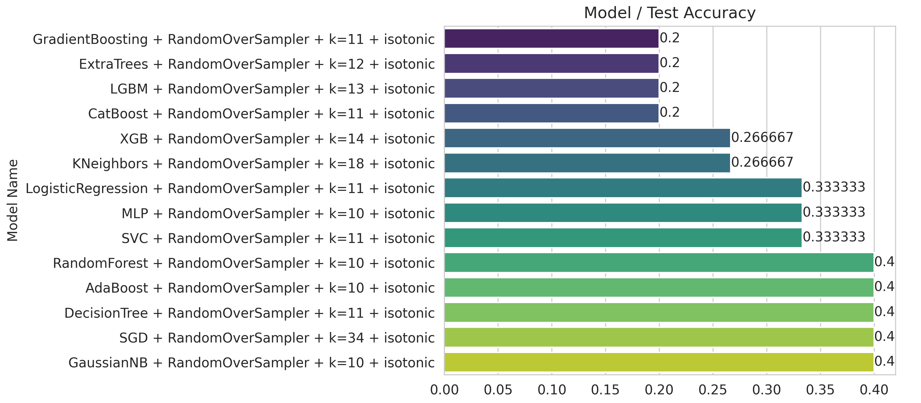
\includegraphics[width=\textwidth]{2014.png}
    \caption{2014 yılına ait model test doğrulukları.}
    \label{fig:resim1}
\end{minipage}
\hfill
\begin{minipage}[b]{0.6\textwidth}
    \centering
    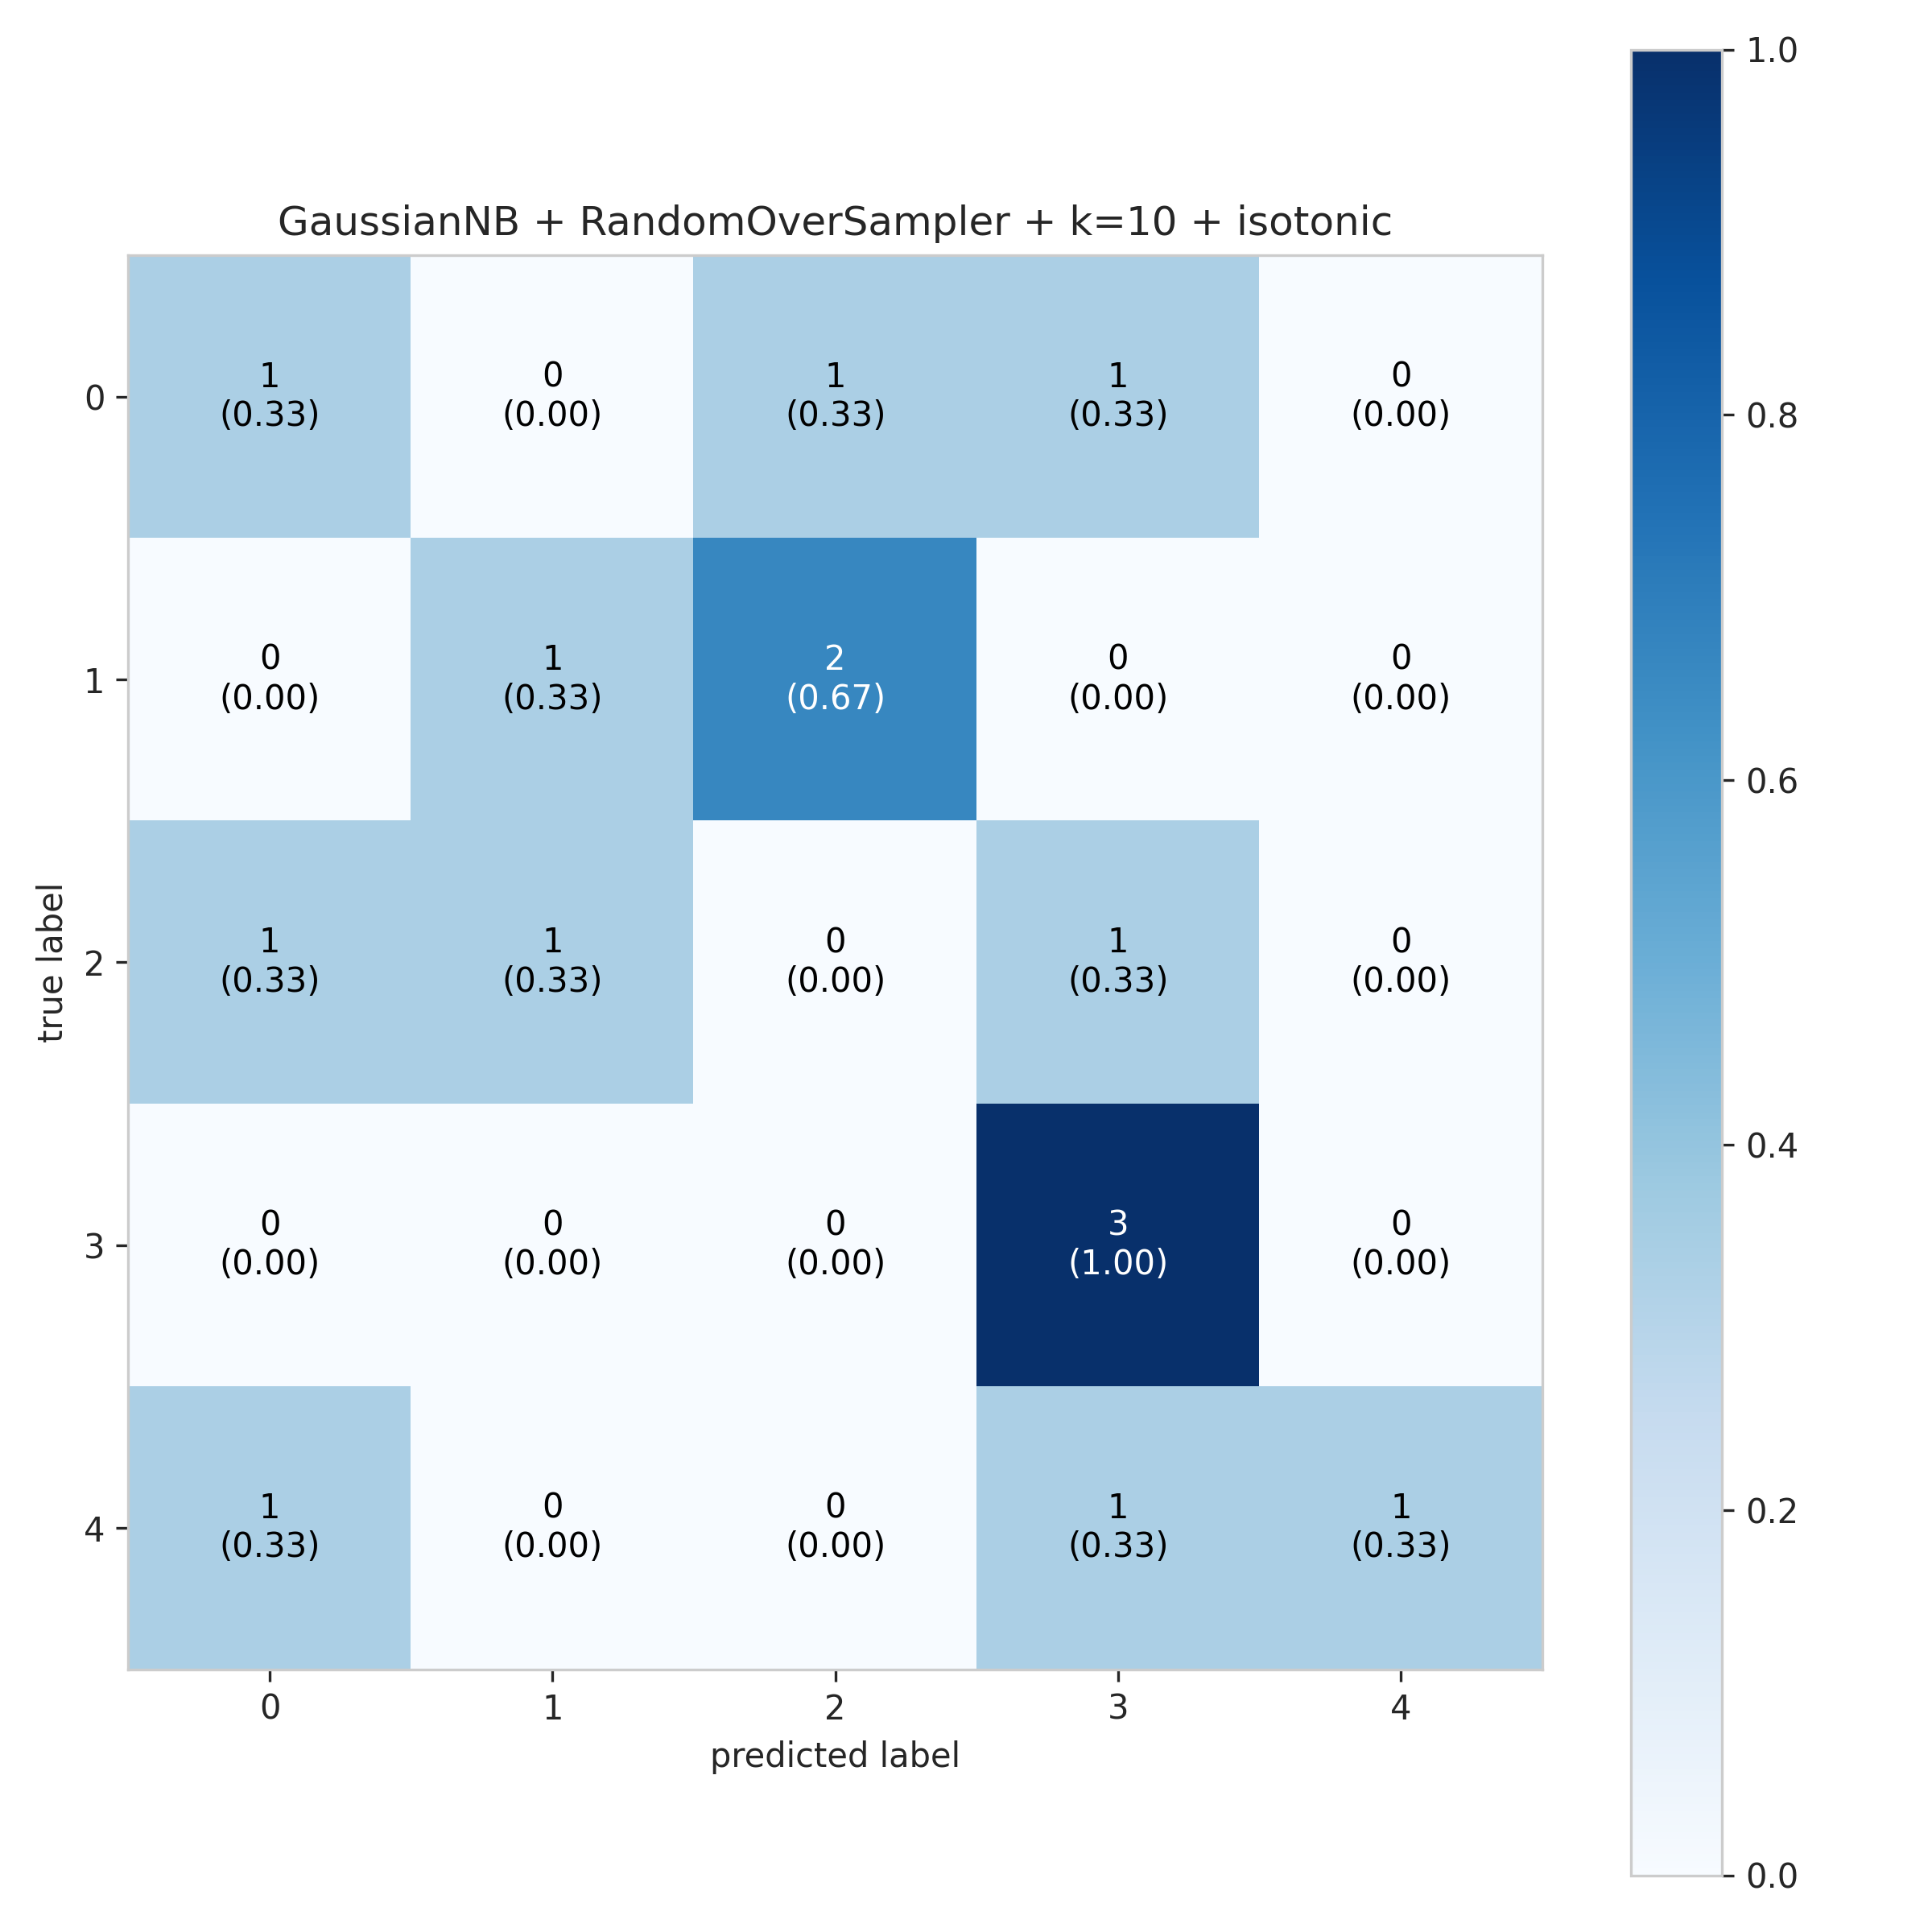
\includegraphics[width=\textwidth]{2014_cm.png}
    \caption{Gaussian Naive Bayes modeline ait karmaşıklık matrisi}
    \label{fig:resim2}
\end{minipage}
\end{figure}

\newpage

\subsection{2015 yılına ait model sonuçları}
2015 yılı için en iyi performansı \%60 sınama doğruluğu,  \%52.14 F1 skoru, \%47 kesinlik skoru ve \%47 duyarlılık skoru ile MLP modeli vermiştir.

\begin{figure}[ht]
\centering
\begin{minipage}[b]{0.6\textwidth}
    \centering
    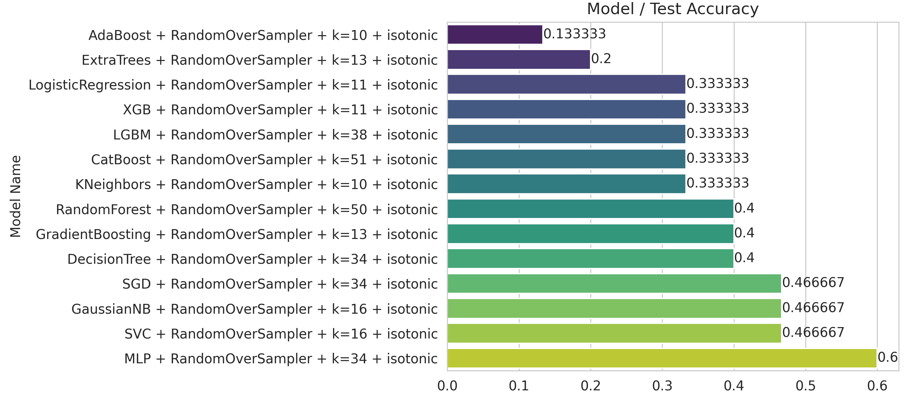
\includegraphics[width=\textwidth]{2015.png}
    \caption{2015 yılına ait model test doğrulukları.}
    \label{fig:resim1}
\end{minipage}
\hfill
\begin{minipage}[b]{0.6\textwidth}
    \centering
    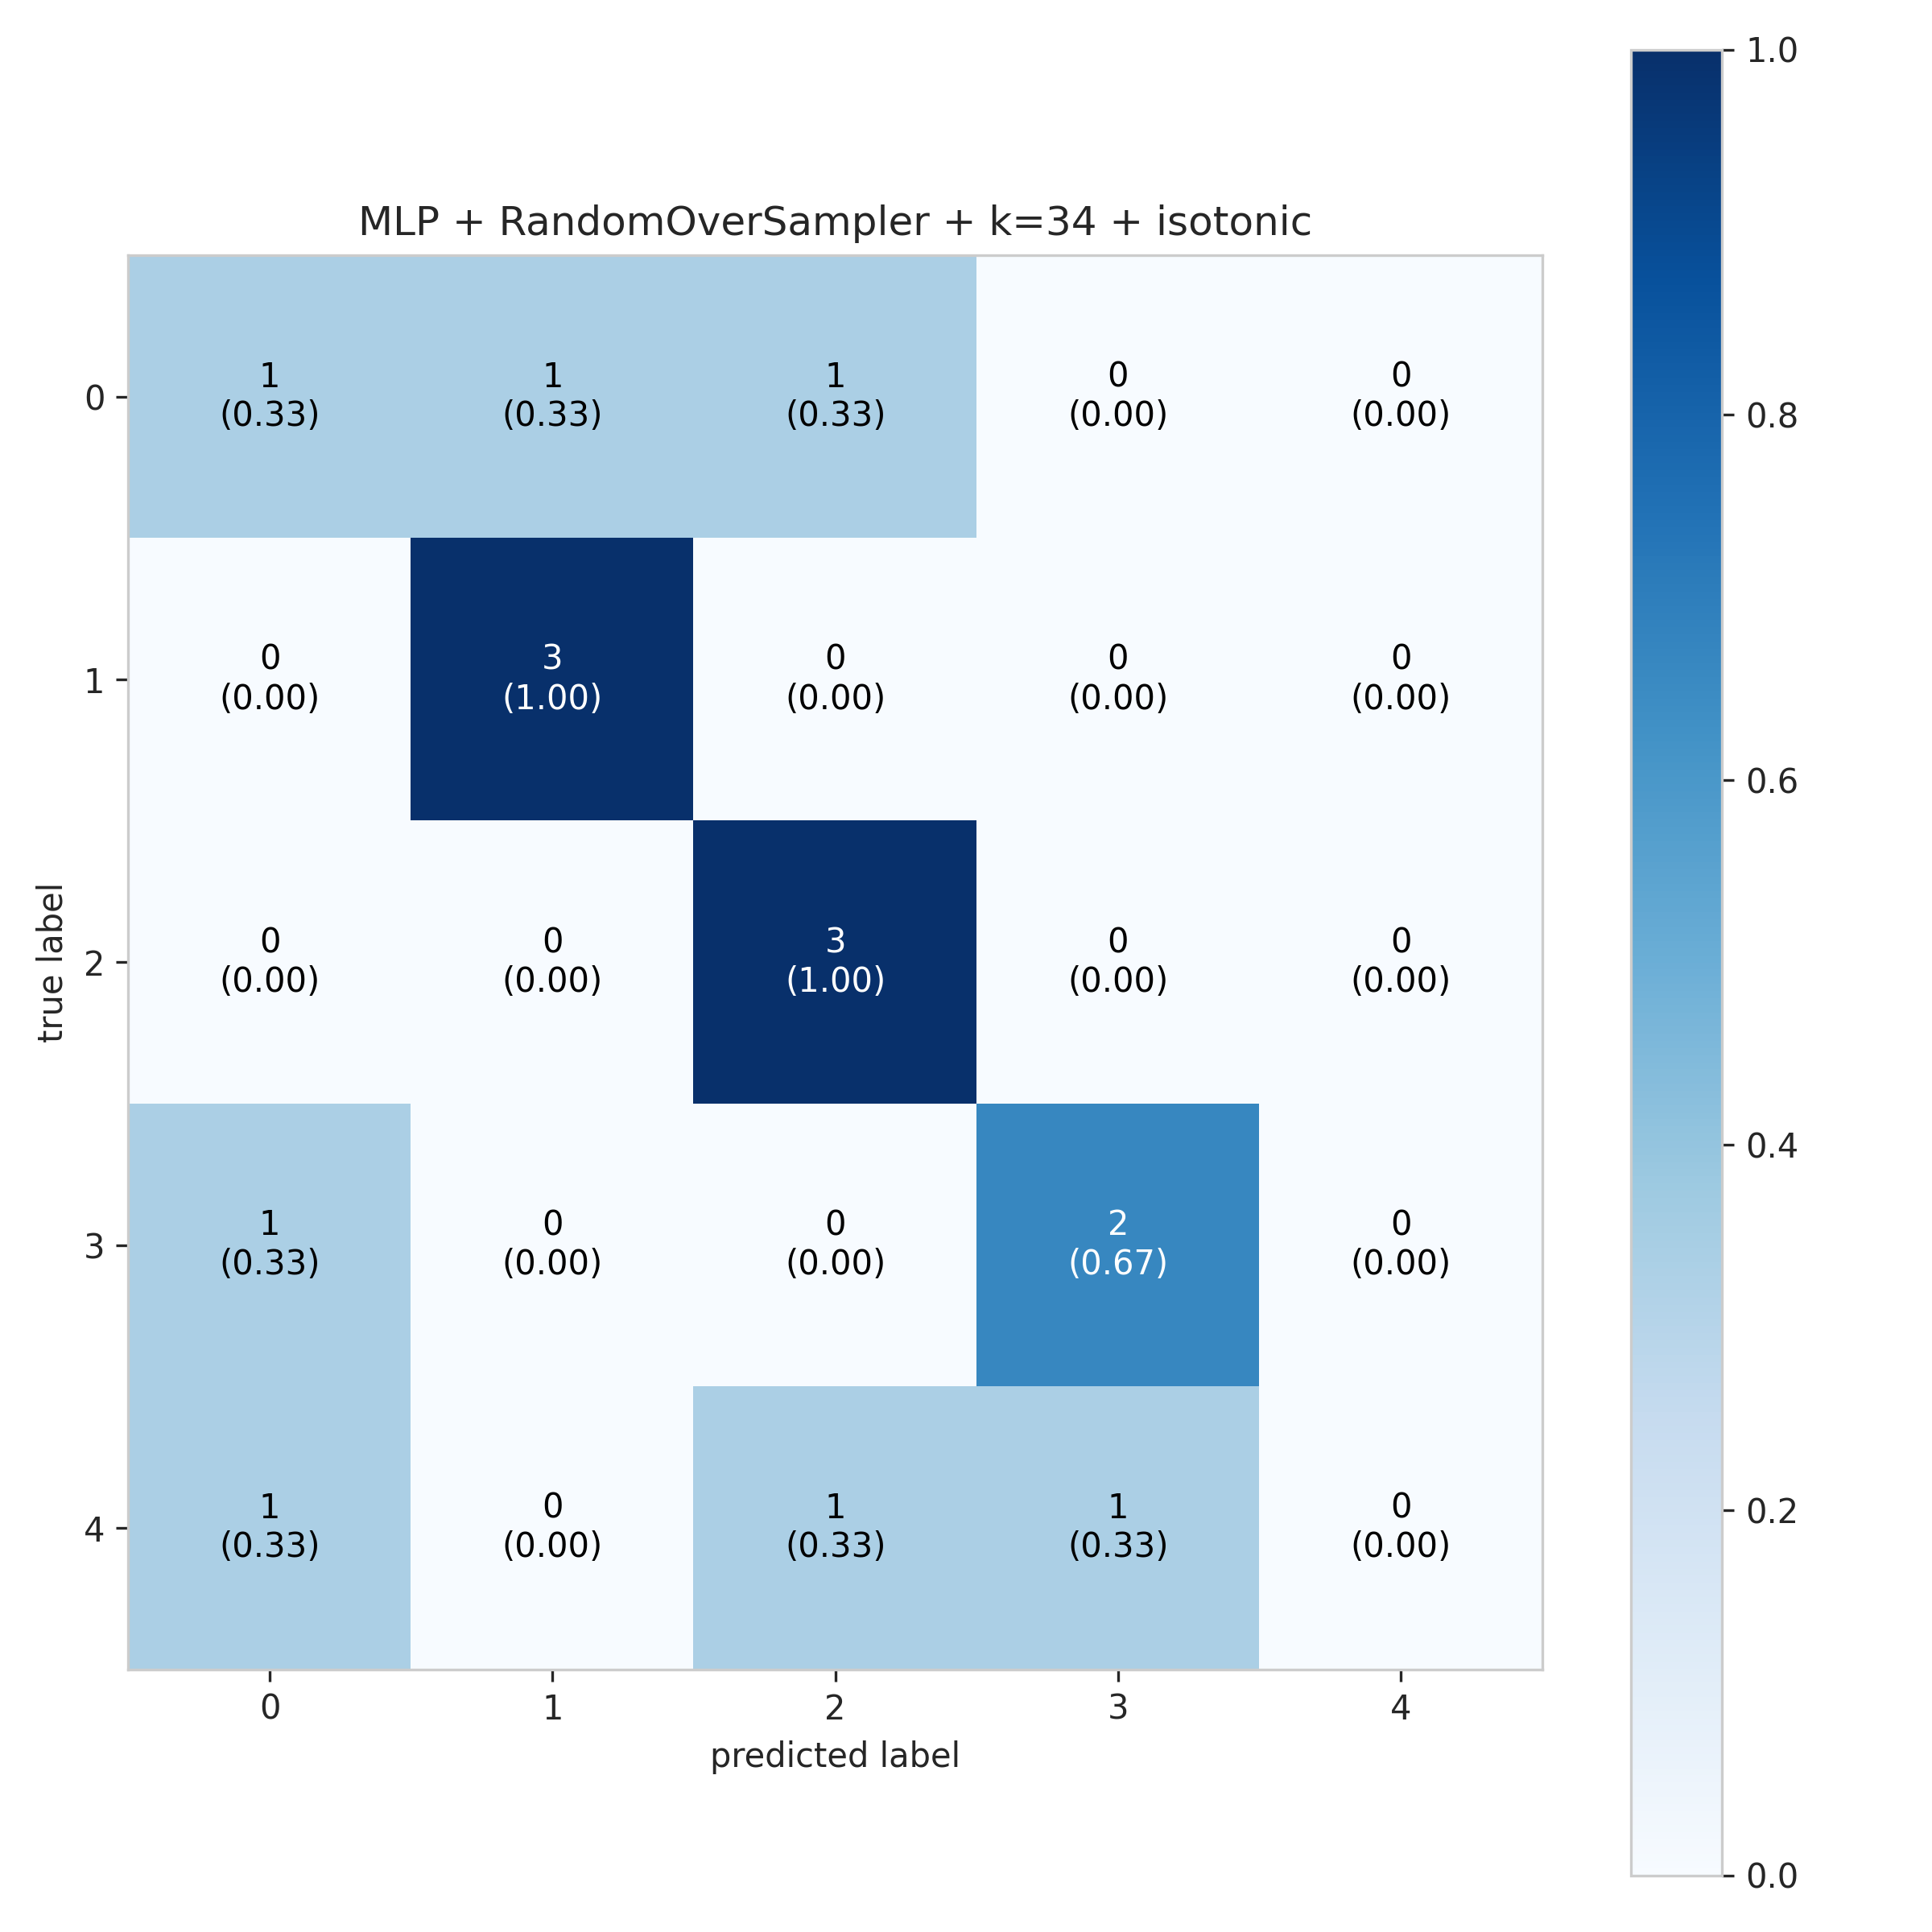
\includegraphics[width=\textwidth]{2015_cm.png}
    \caption{MLP modeline ait karmaşıklık matrisi}
    \label{fig:resim2}
\end{minipage}
\end{figure}

\newpage

\subsection{2016 yılına ait model sonuçları}
2016 yılı için en iyi performansı \%66.66 sınama doğruluğu,  \%65.23 F1 skoru, \%71.66 kesinlik skoru ve \%71.66 duyarlılık skoru ile SVC modeli vermiştir.

\begin{figure}[ht]
\centering
\begin{minipage}[b]{0.6\textwidth}
    \centering
    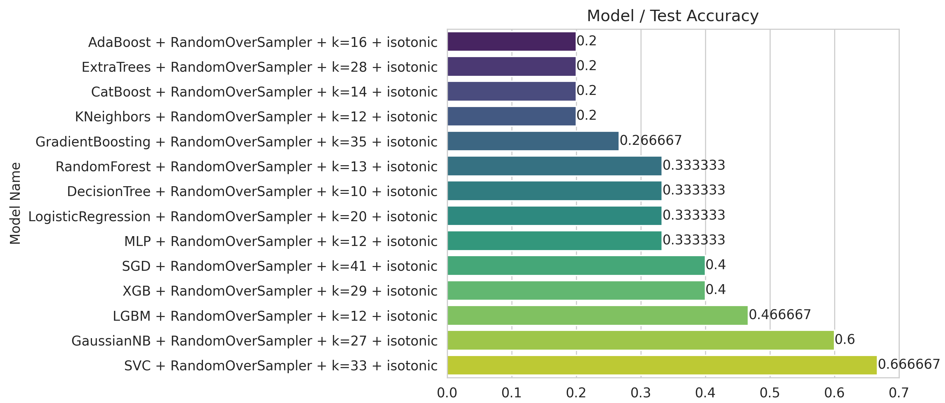
\includegraphics[width=\textwidth]{2016.png}
    \caption{2016 yılına ait model test doğrulukları.}
    \label{fig:resim1}
\end{minipage}
\hfill
\begin{minipage}[b]{0.6\textwidth}
    \centering
    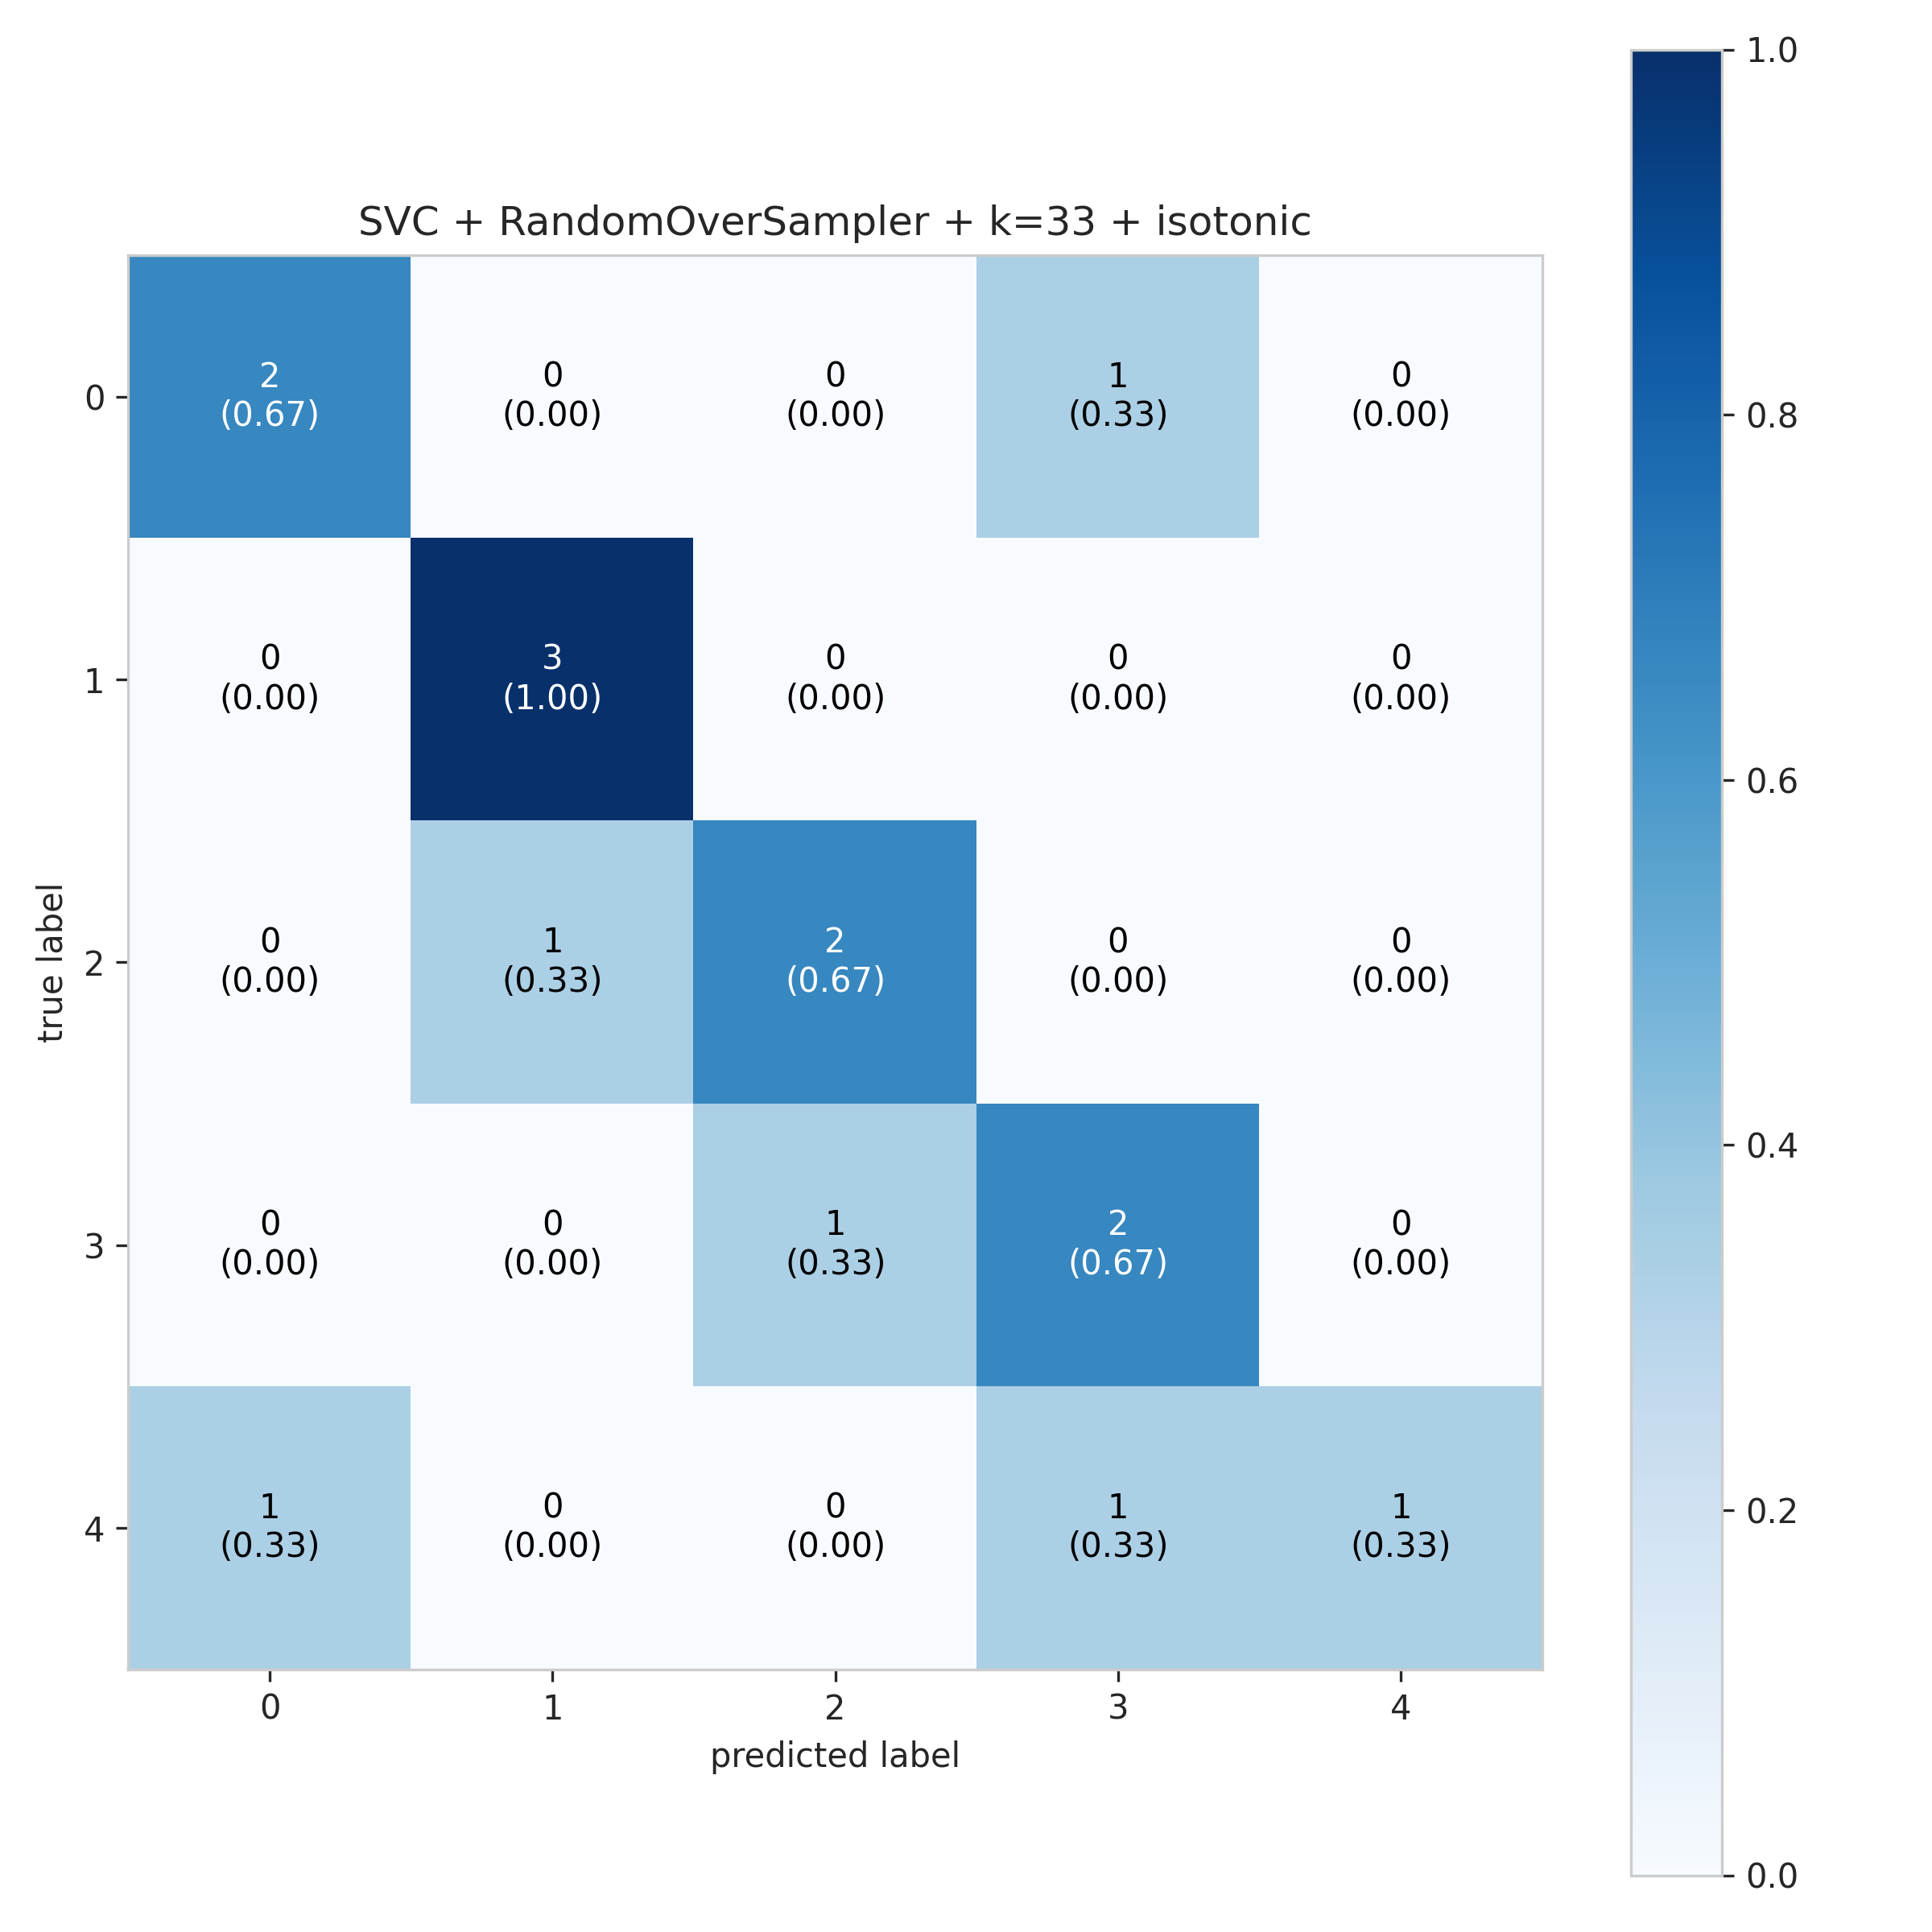
\includegraphics[width=\textwidth]{2016_cm.png}
    \caption{SVC modeline ait karmaşıklık matrisi}
    \label{fig:resim2}
\end{minipage}
\end{figure}

\newpage

\subsection{2017 yılına ait model sonuçları}
2017 yılı için en iyi performansı \%53.33 sınama doğruluğu,  \%45.90 F1 skoru, \%59.5 kesinlik skoru ve \%59.5 duyarlılık skoru ile MLP modeli vermiştir.

\begin{figure}[ht]
\centering
\begin{minipage}[b]{0.6\textwidth}
    \centering
    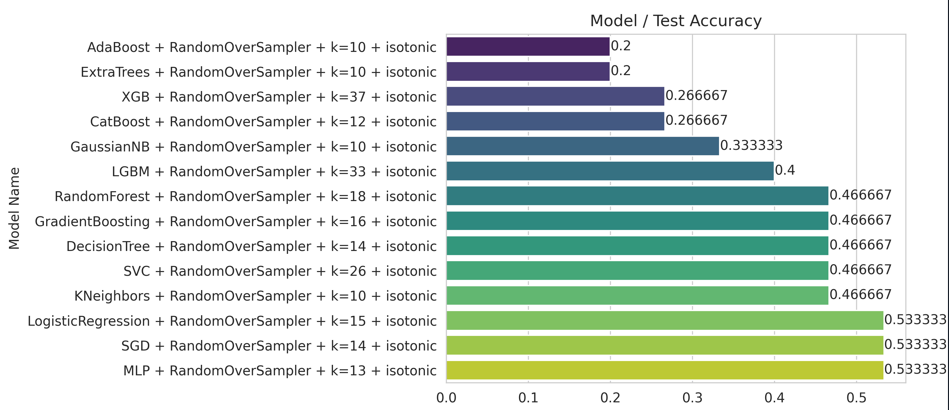
\includegraphics[width=\textwidth]{2017.png}
    \caption{2017 yılına ait model test doğrulukları.}
    \label{fig:resim1}
\end{minipage}
\hfill
\begin{minipage}[b]{0.6\textwidth}
    \centering
    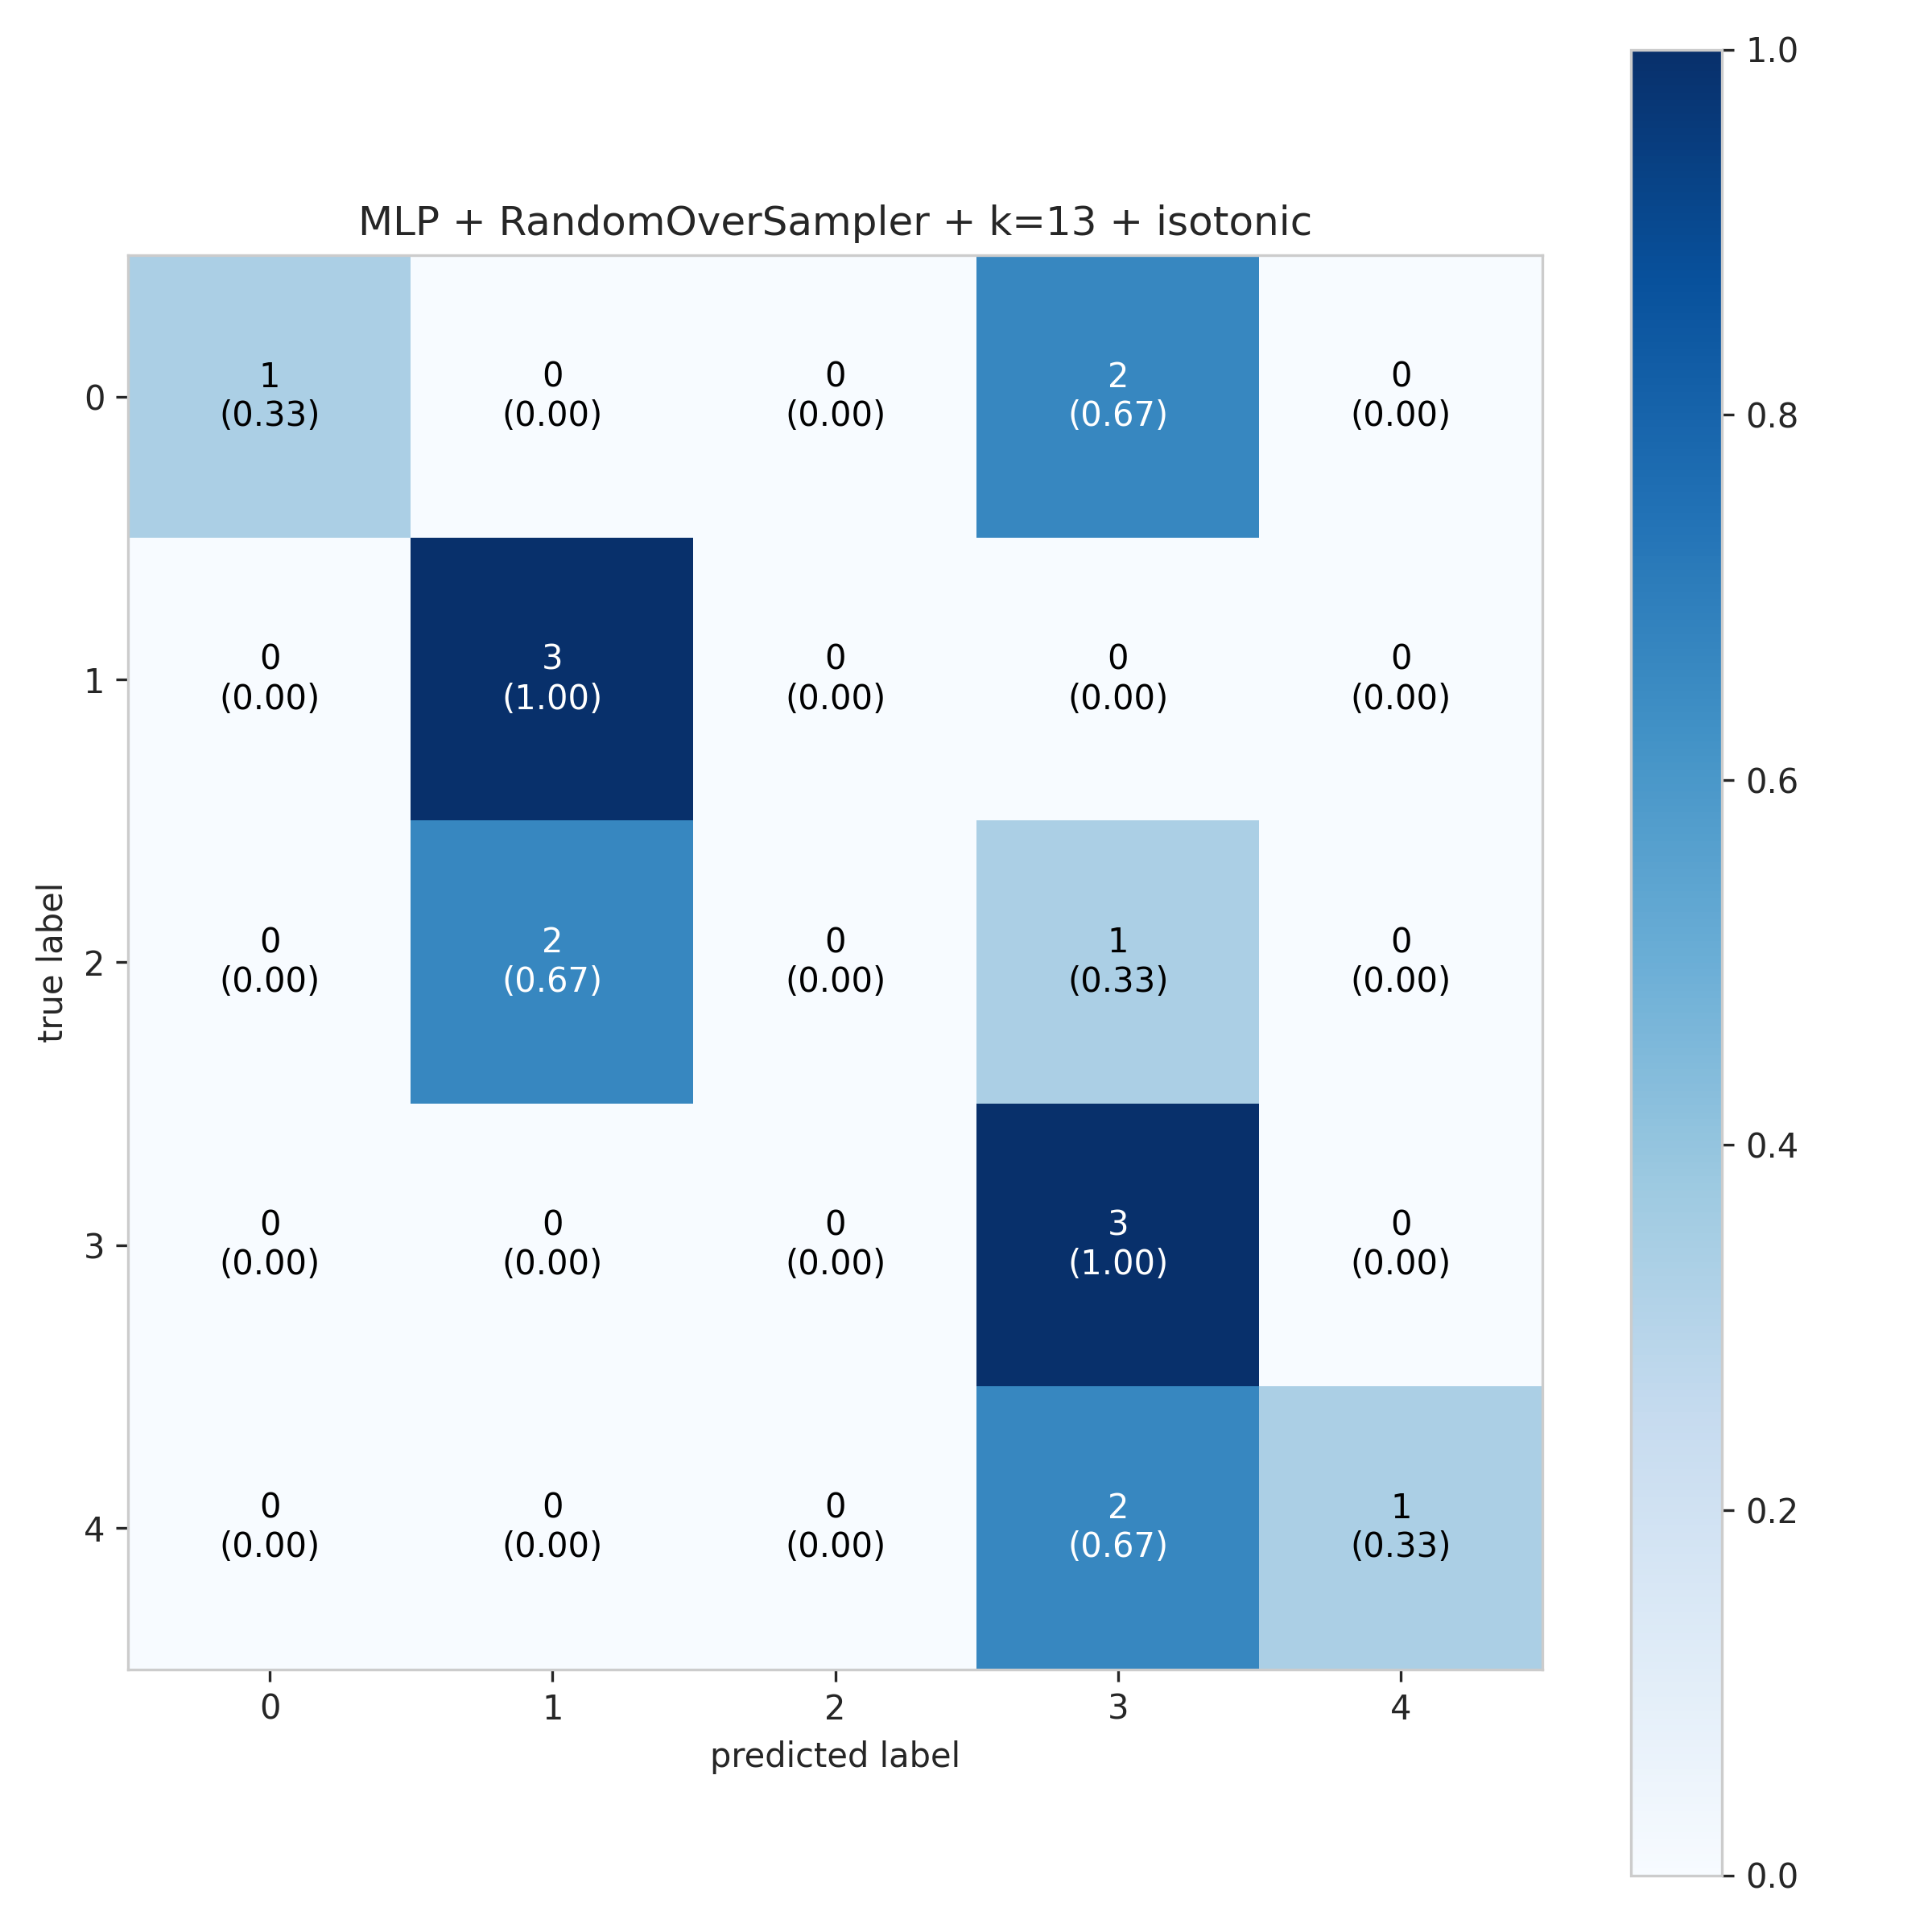
\includegraphics[width=\textwidth]{2017_cm.png}
    \caption{MLP modeline ait karmaşıklık matrisi}
    \label{fig:resim2}
\end{minipage}
\end{figure}

\newpage

\subsection{2018 yılına ait model sonuçları}
2018 yılı için en iyi performansı \%53.33 sınama doğruluğu,  \%53.65 F1 skoru, \%70 kesinlik skoru ve \%70 duyarlılık skoru ile KNeighbors modeli vermiştir.

\begin{figure}[ht]
\centering
\begin{minipage}[b]{0.6\textwidth}
    \centering
    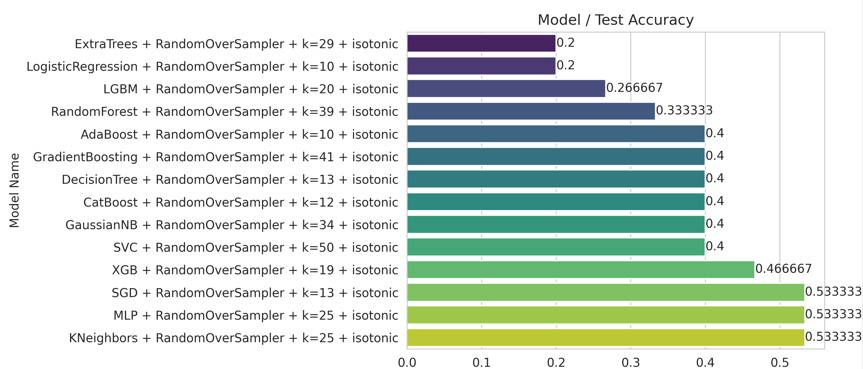
\includegraphics[width=\textwidth]{2018.png}
    \caption{2018 yılına ait model test doğrulukları.}
    \label{fig:resim1}
\end{minipage}
\hfill
\begin{minipage}[b]{0.6\textwidth}
    \centering
    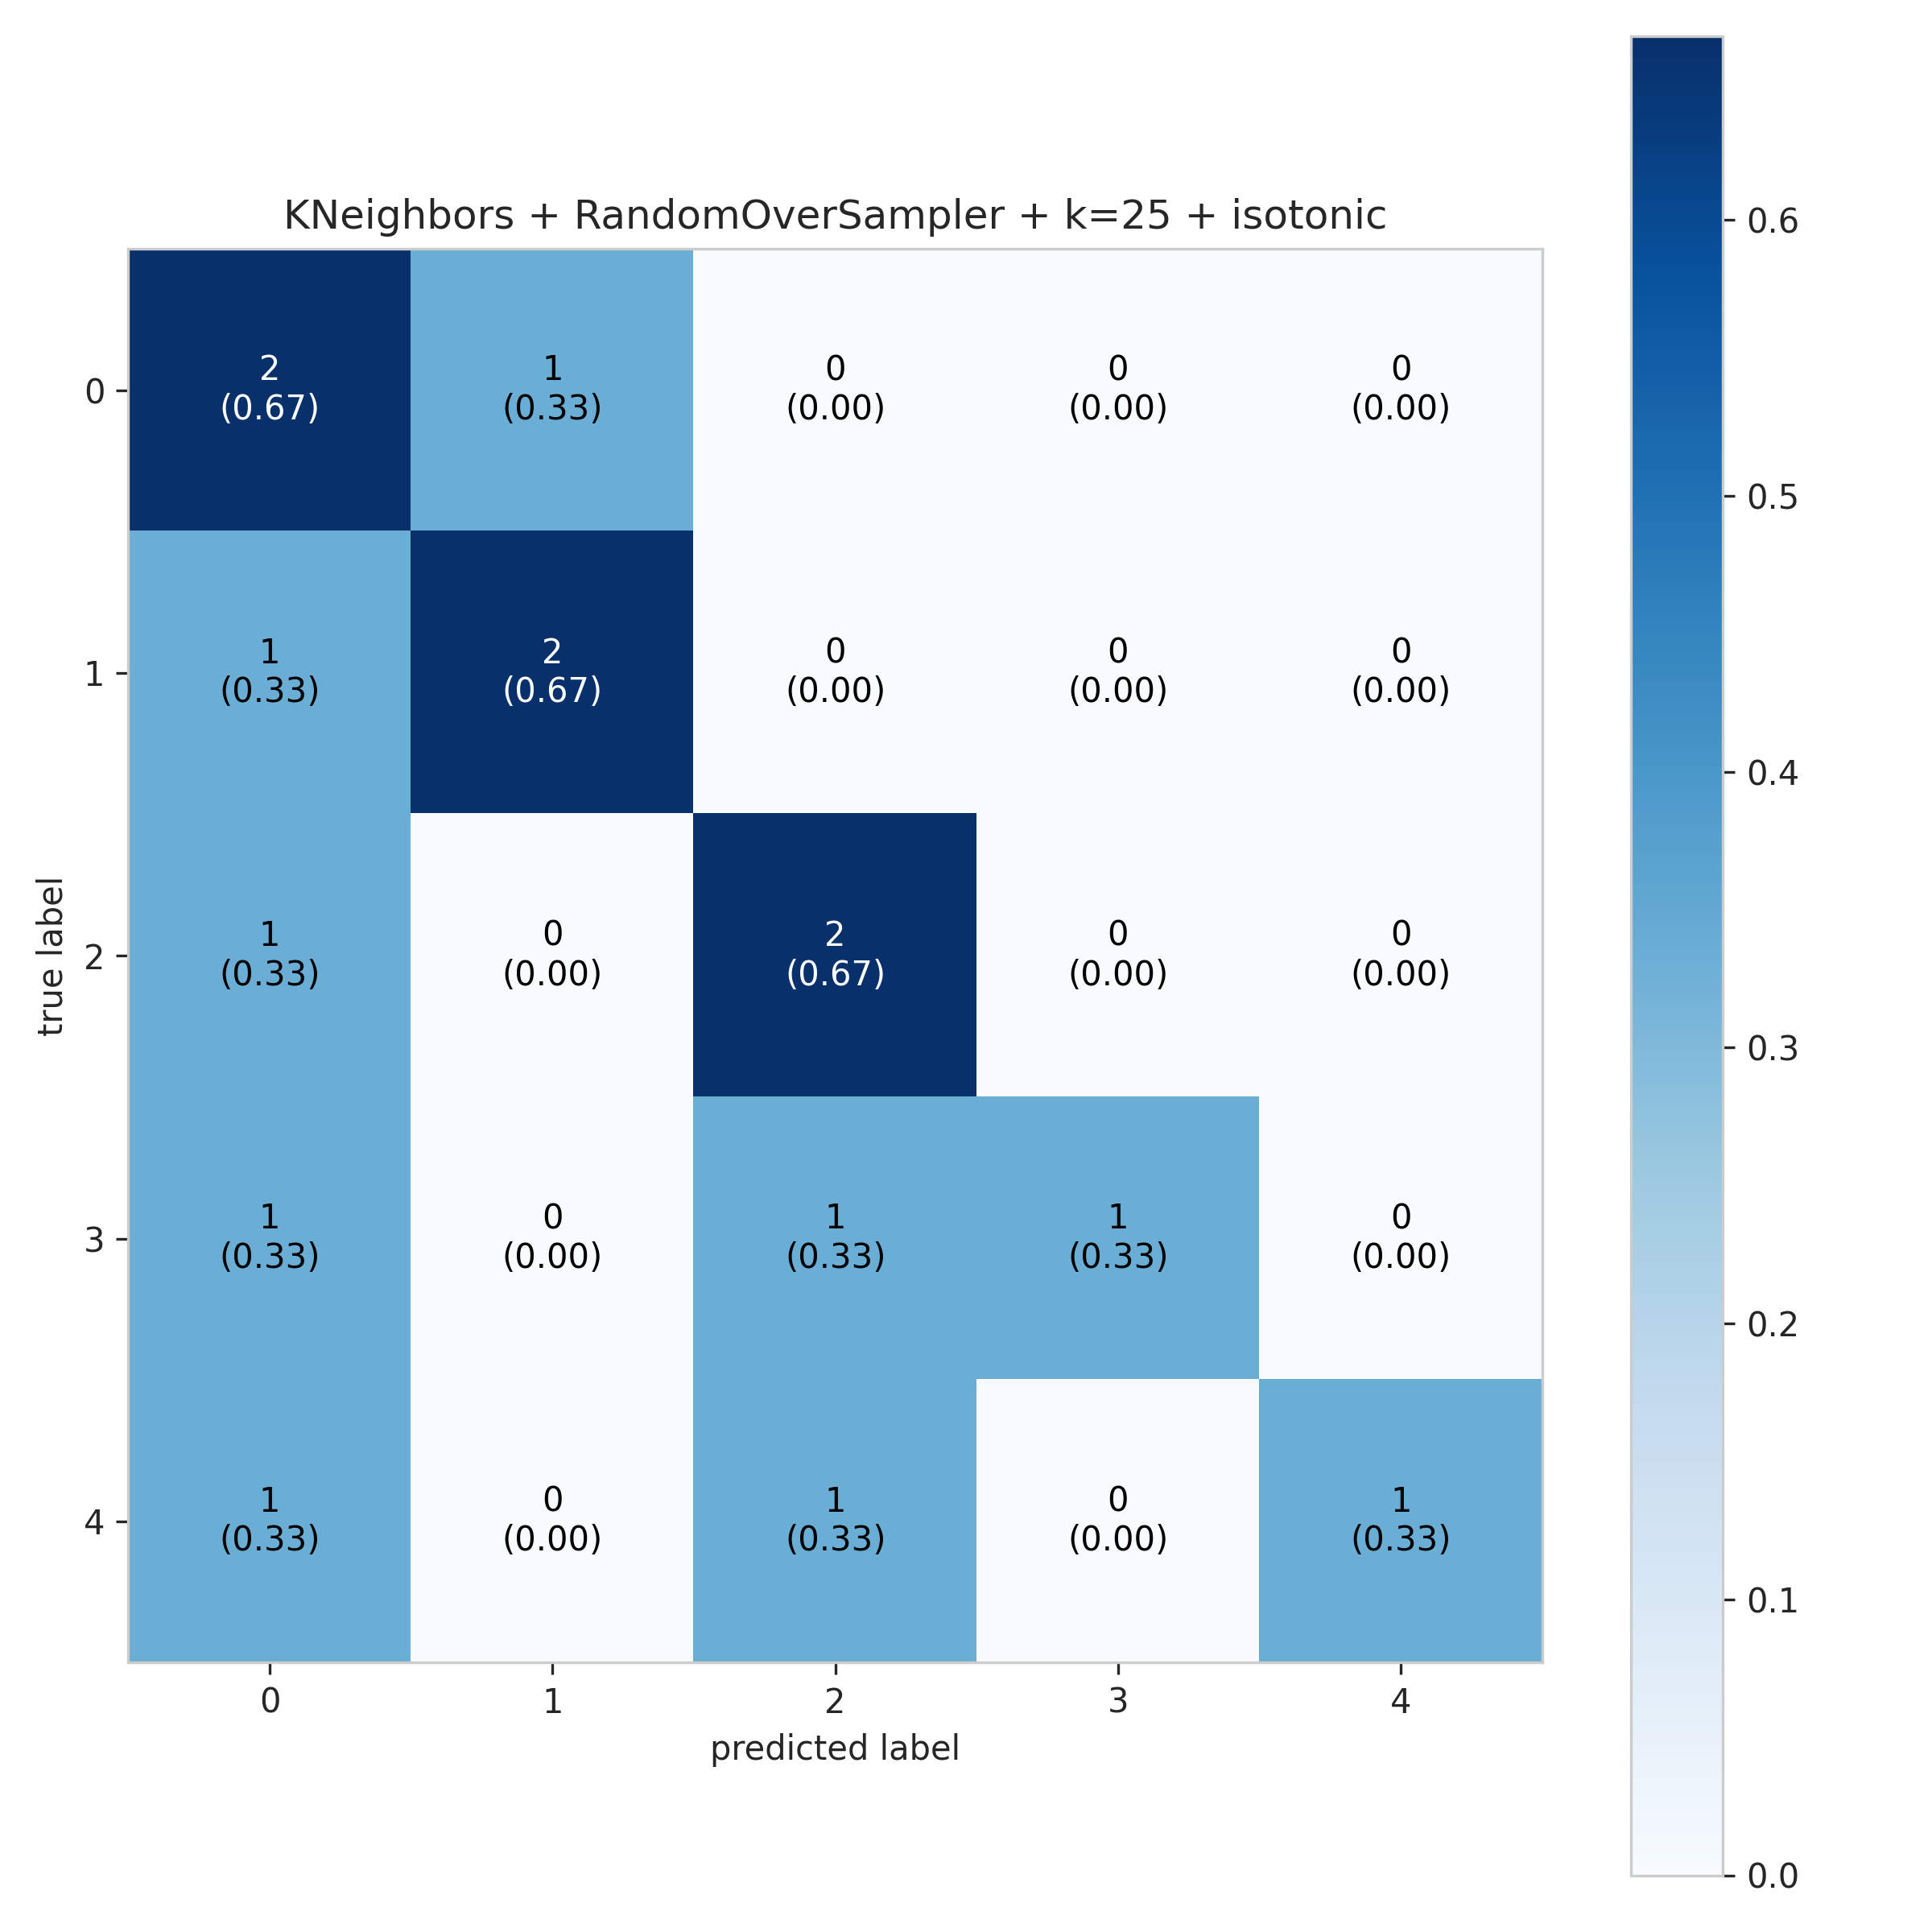
\includegraphics[width=\textwidth]{2018_cm.png}
    \caption{KNeighbors modeline ait karmaşıklık matrisi}
    \label{fig:resim2}
\end{minipage}
\end{figure}

\newpage

\subsection{2019 yılına ait model sonuçları}
2019 yılı için en iyi performansı \%53.33 sınama doğruluğu,  \%52 F1 skoru, \%68.57 kesinlik skoru ve \%68.57 duyarlılık skoru ile XGB modeli vermiştir.

\begin{figure}[ht]
\centering
\begin{minipage}[b]{0.6\textwidth}
    \centering
    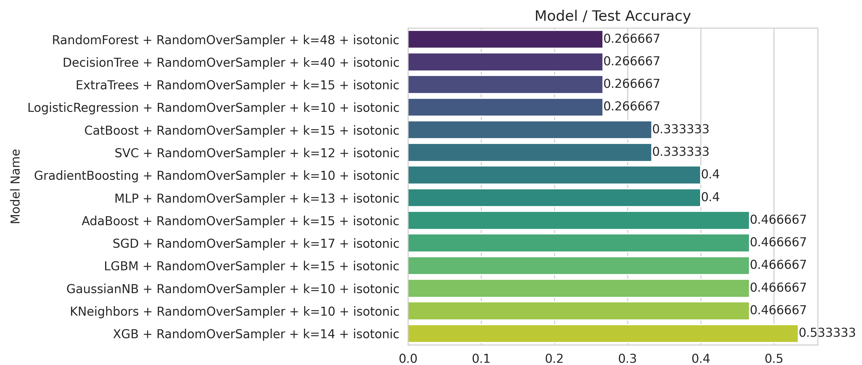
\includegraphics[width=\textwidth]{2019.png}
    \caption{2019 yılına ait model test doğrulukları.}
    \label{fig:resim1}
\end{minipage}
\hfill
\begin{minipage}[b]{0.6\textwidth}
    \centering
    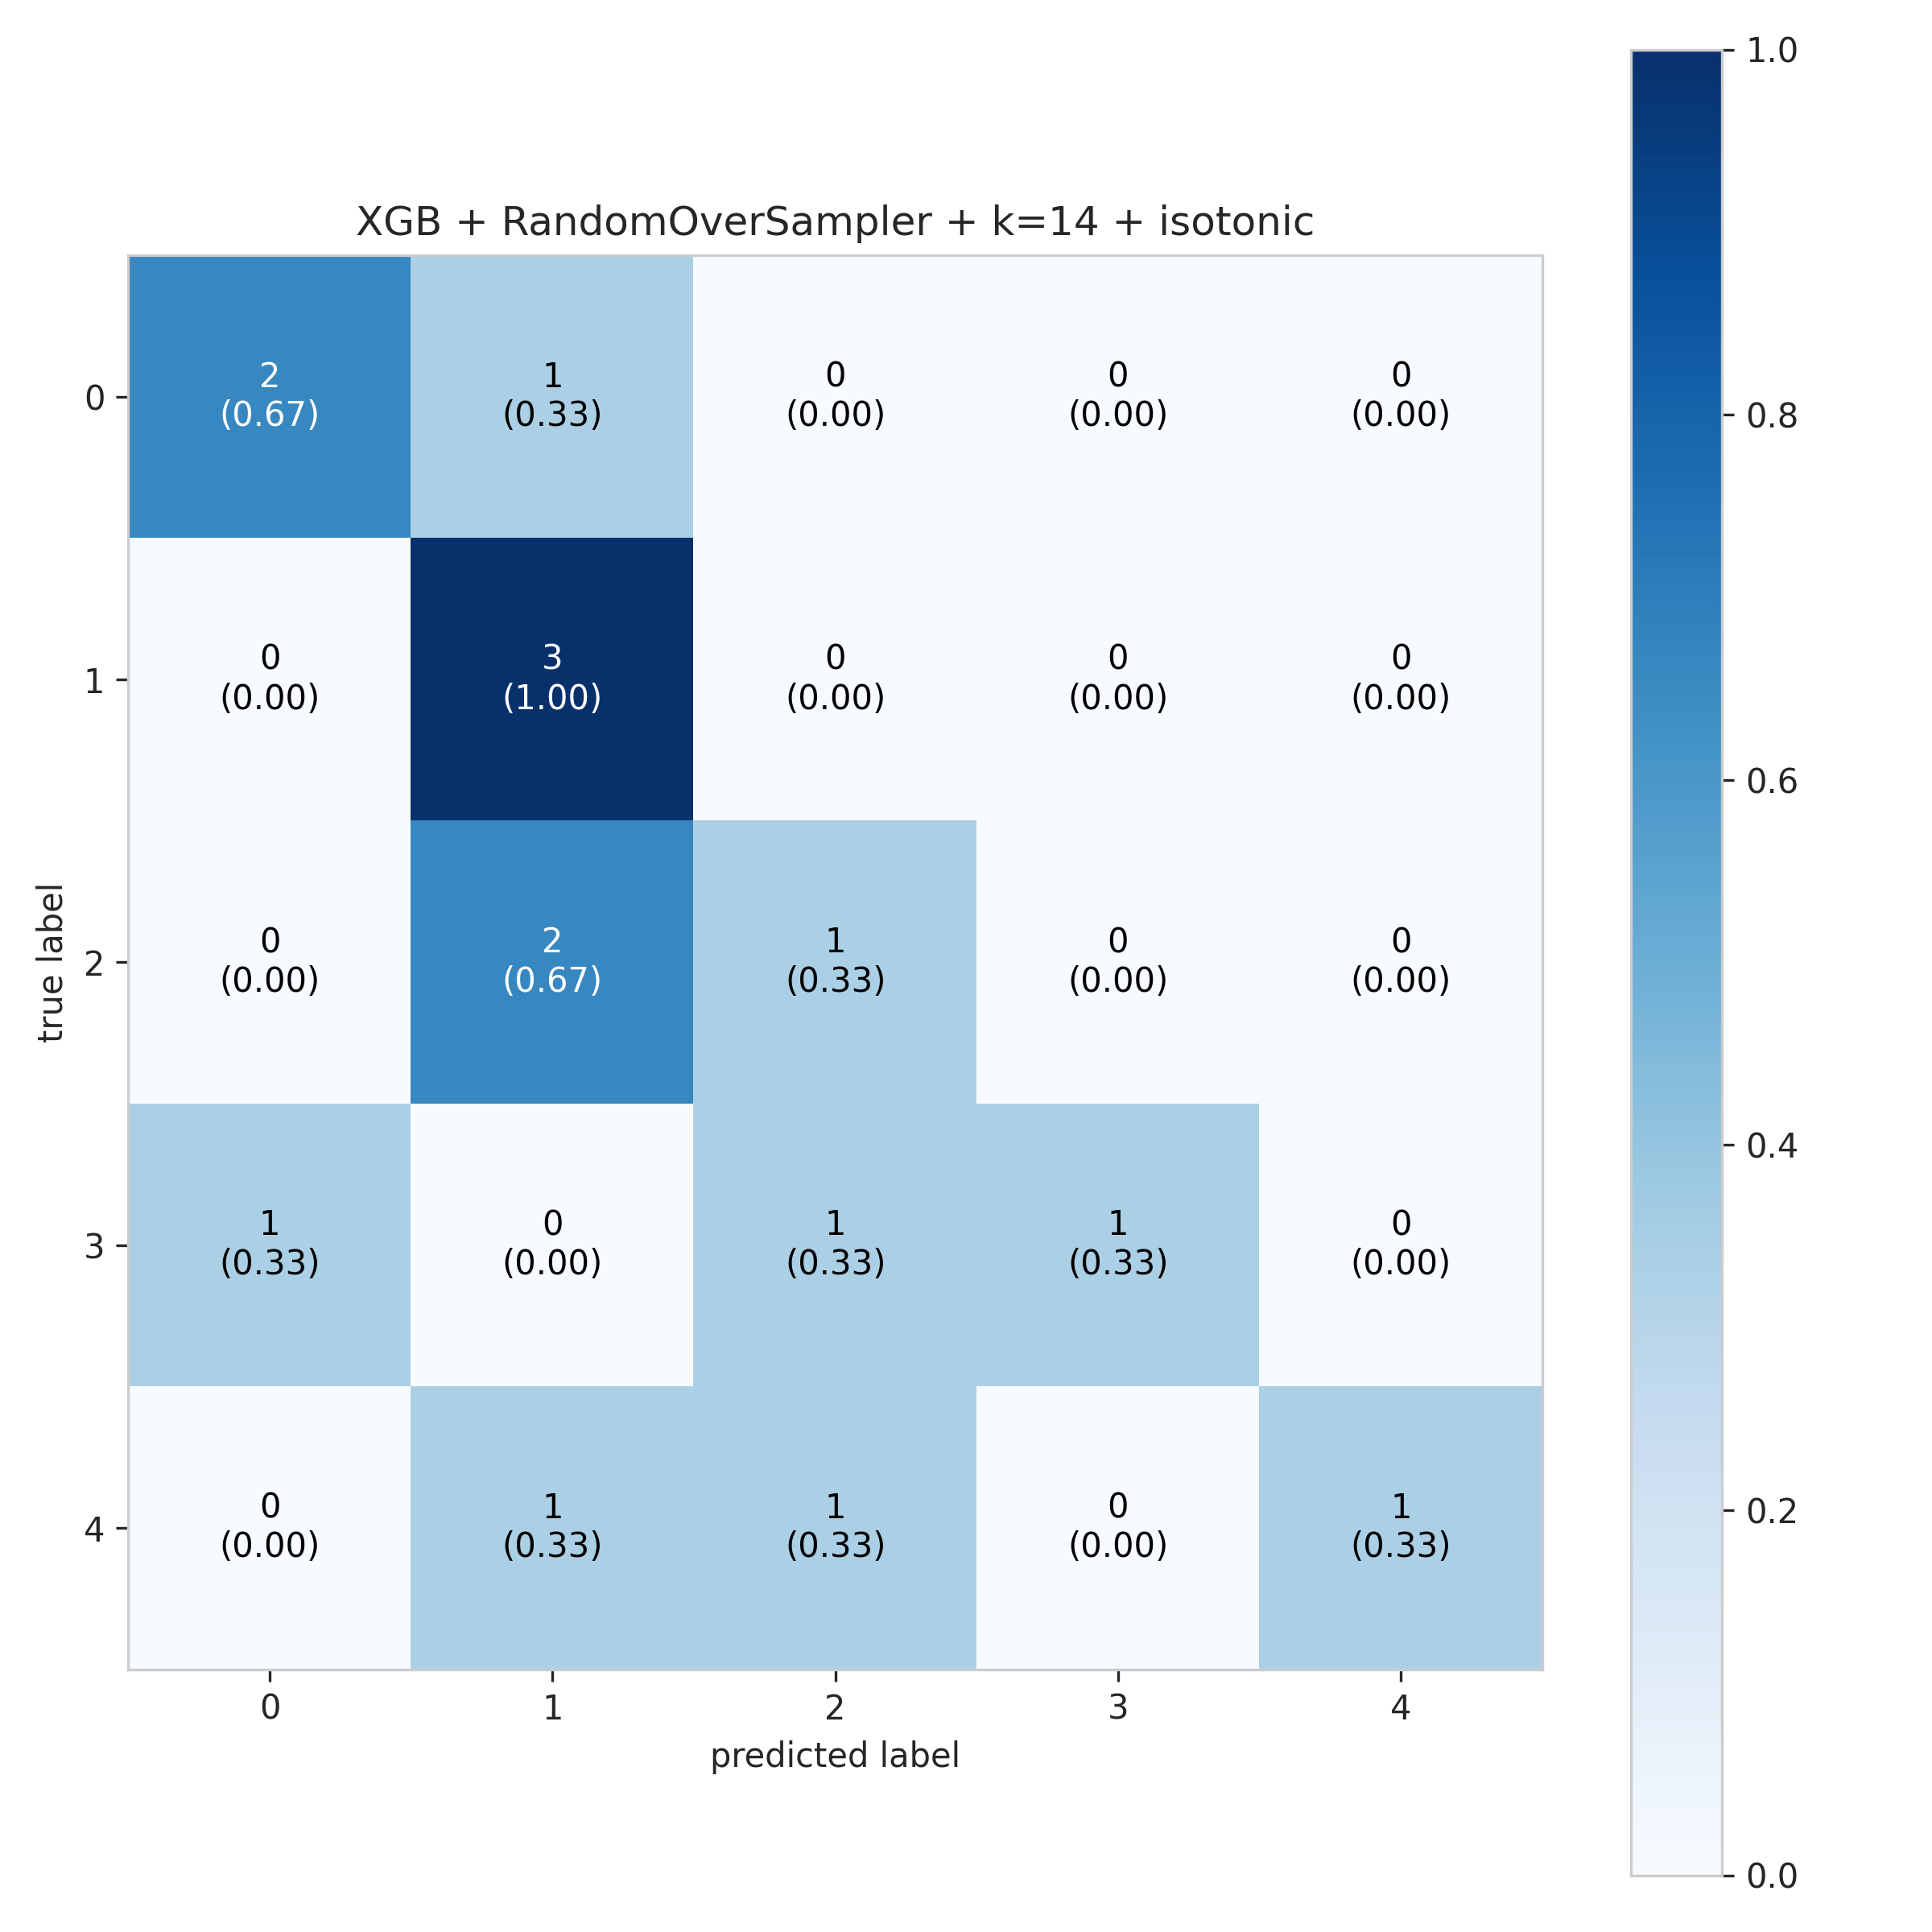
\includegraphics[width=\textwidth]{2019_cm.png}
    \caption{XGB modeline ait karmaşıklık matrisi}
    \label{fig:resim2}
\end{minipage}
\end{figure}

\newpage

\subsection{2020 yılına ait model sonuçları}
2020 yılı için en iyi performansı \%60 sınama doğruluğu,  \%58.33 F1 skoru, \%73.33 kesinlik skoru ve \%73.33 duyarlılık skoru ile MLP modeli vermiştir.

\begin{figure}[ht]
\centering
\begin{minipage}[b]{0.6\textwidth}
    \centering
    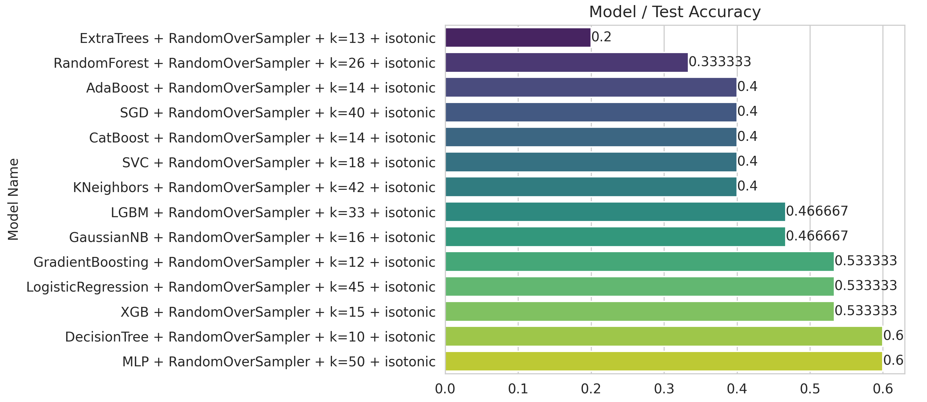
\includegraphics[width=\textwidth]{2020.png}
    \caption{2020 yılına ait model test doğrulukları.}
    \label{fig:resim1}
\end{minipage}
\hfill
\begin{minipage}[b]{0.6\textwidth}
    \centering
    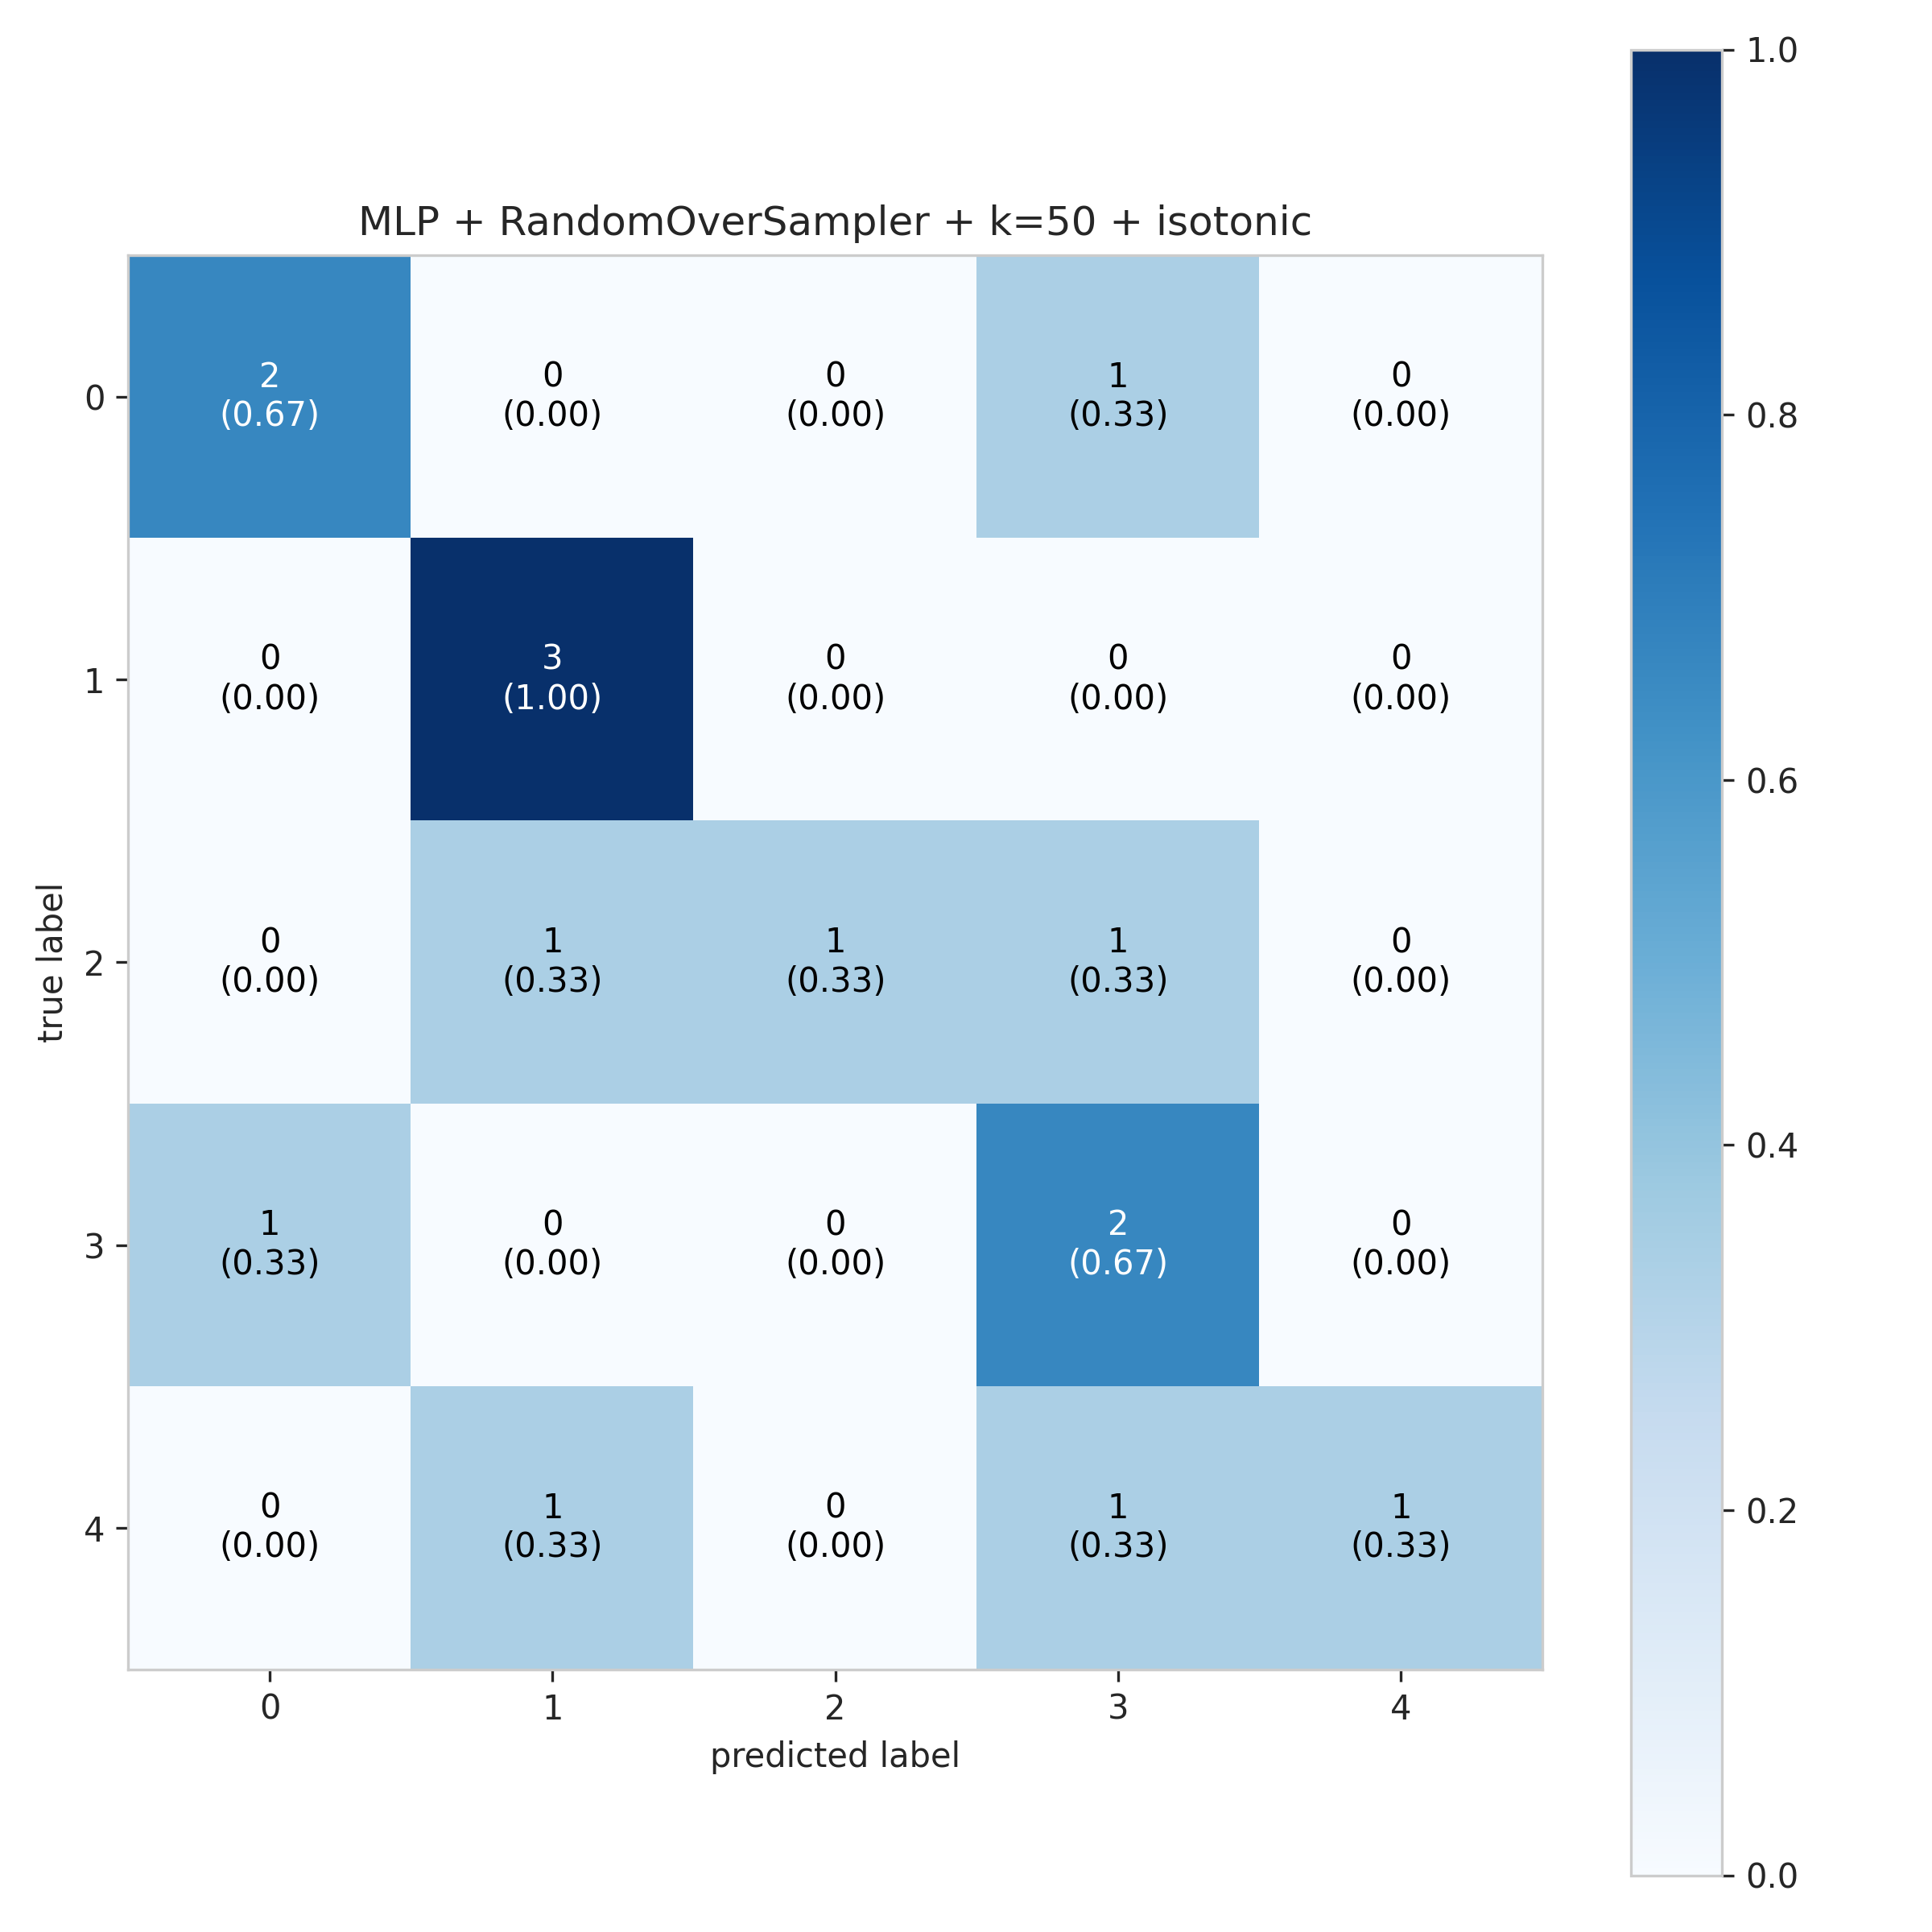
\includegraphics[width=\textwidth]{2020_cm.png}
    \caption{MLP modeline ait karmaşıklık matrisi}
    \label{fig:resim2}
\end{minipage}
\end{figure}

\newpage

\subsection{2021 yılına ait model sonuçları}
2021 yılı için en iyi performansı \%53.33 sınama doğruluğu,  \%49.71 F1 skoru, \%53.57 kesinlik skoru ve \%53.57 duyarlılık skoru ile LGBM modeli vermiştir.

\begin{figure}[ht]
\centering
\begin{minipage}[b]{0.6\textwidth}
    \centering
    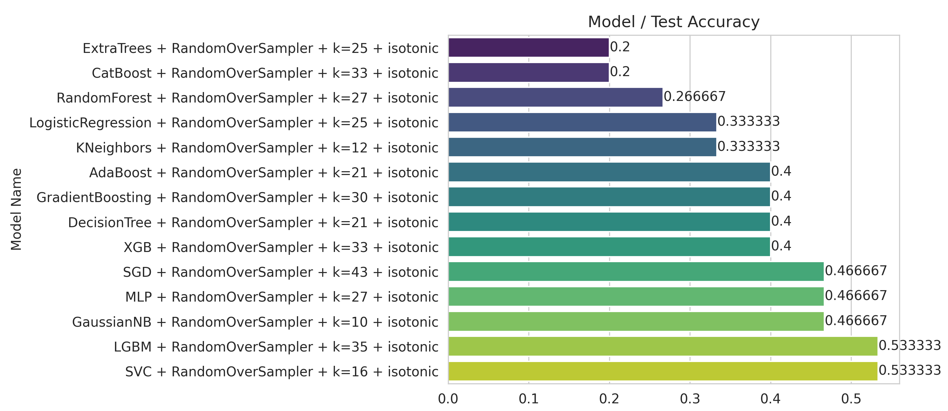
\includegraphics[width=\textwidth]{2021.png}
    \caption{2021 yılına ait model test doğrulukları.}
    \label{fig:resim1}
\end{minipage}
\hfill
\begin{minipage}[b]{0.6\textwidth}
    \centering
    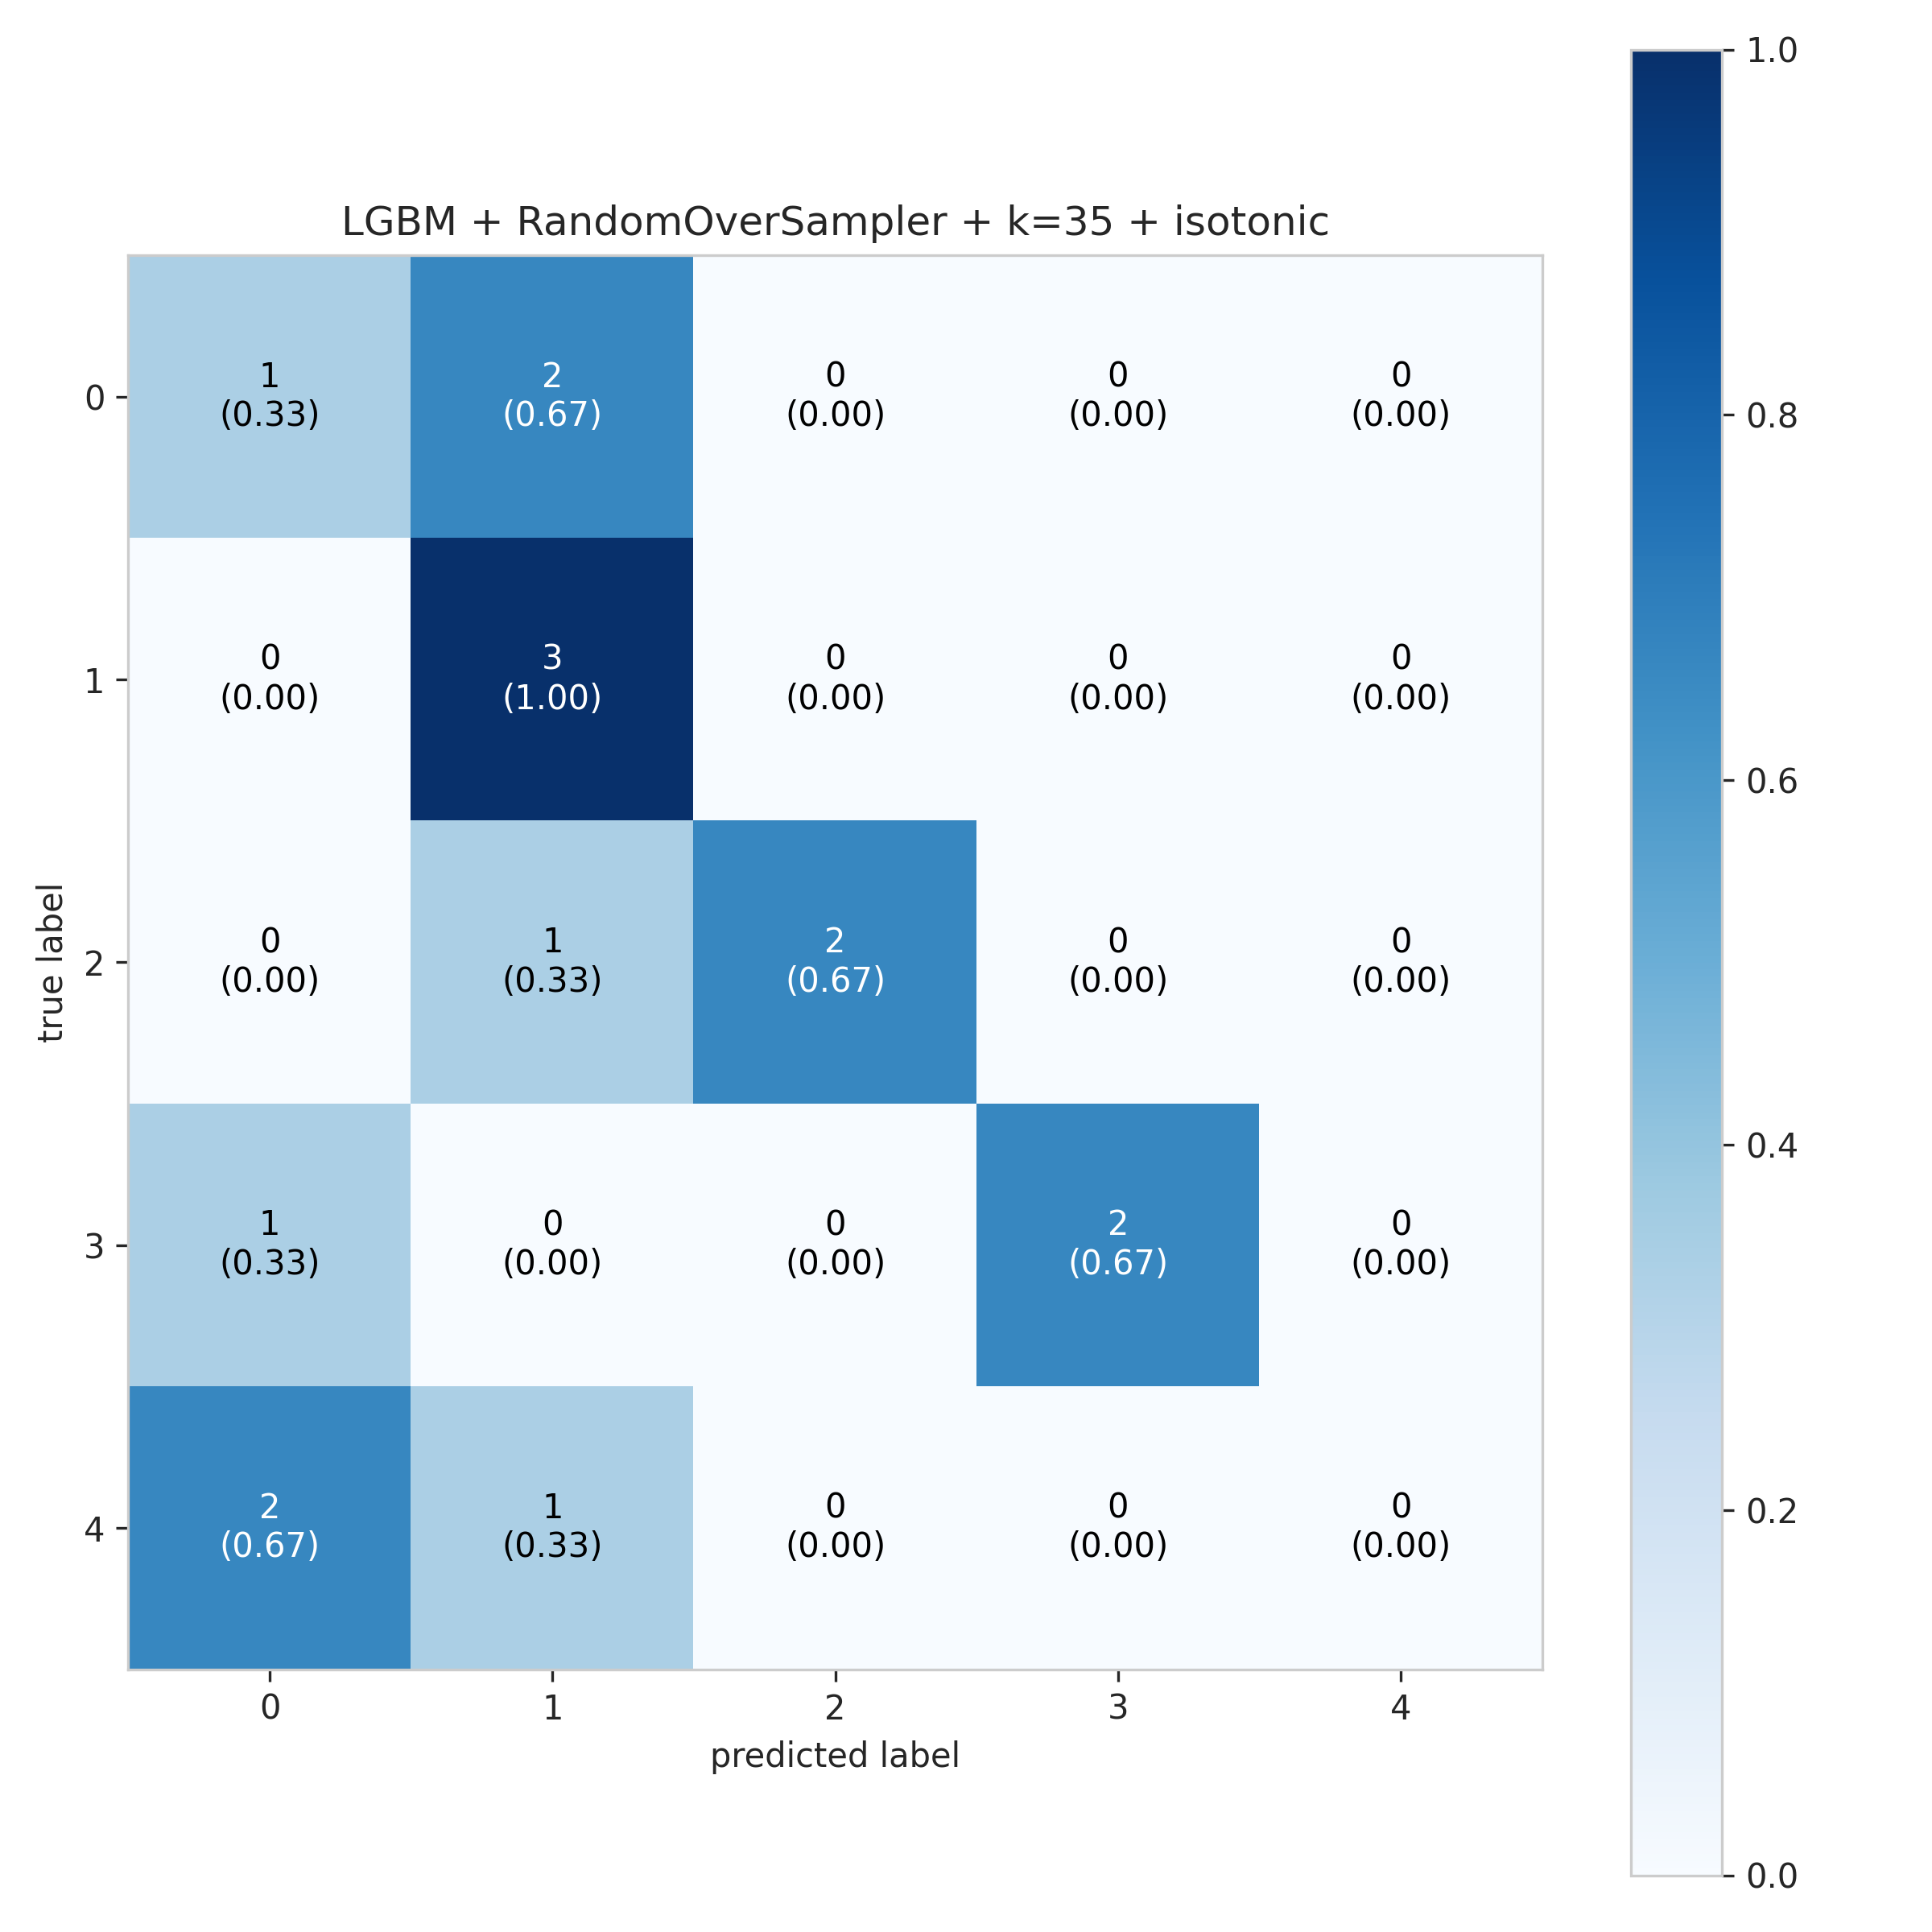
\includegraphics[width=\textwidth]{2021_cm.png}
    \caption{LGBM modeline ait karmaşıklık matrisi}
    \label{fig:resim2}
\end{minipage}
\end{figure}

\newpage

\subsection{2022 yılına ait model sonuçları}
2022 yılı için en iyi performansı \%33.33 sınama doğruluğu,  \%27.5 F1 skoru, \%44.61 kesinlik skoru ve \%44.61 duyarlılık skoru ile KNeighbors modeli vermiştir.

\begin{figure}[ht]
\centering
\begin{minipage}[b]{0.6\textwidth}
    \centering
    \includegraphics[width=\textwidth]{2022.png}
    \caption{2022 yılına ait model test doğrulukları.}
    \label{fig:resim1}
\end{minipage}
\hfill
\begin{minipage}[b]{0.6\textwidth}
    \centering
    \includegraphics[width=\textwidth]{2022_cm.png}
    \caption{KNeighbors modeline ait karmaşıklık matrisi}
    \label{fig:resim2}
\end{minipage}
\end{figure}

\newpage

\subsection{2023 yılına ait model sonuçları}
2023 yılı için en iyi performansı \%46.66 sınama doğruluğu,  \%39.76 F1 skoru, \%35.33 kesinlik skoru ve \%35.33 duyarlılık skoru ile Random Forest modeli vermiştir.

\begin{figure}[ht]
\centering
\begin{minipage}[b]{0.6\textwidth}
    \centering
    \includegraphics[width=\textwidth]{2023.png}
    \caption{2023 yılına ait model test doğrulukları.}
    \label{fig:resim1}
\end{minipage}
\hfill
\begin{minipage}[b]{0.6\textwidth}
    \centering
    \includegraphics[width=\textwidth]{2023_cm.png}
    \caption{Random Forest modeline ait karmaşıklık matrisi}
    \label{fig:resim2}
\end{minipage}
\end{figure}

\newpage

\subsection{Sonuç}
Yıllara göre en iyi modeller ve skorları aşağıdaki tabloda verilmiştir.

\begin{table}[h]
\caption{Yıllara göre en iyi modeller.}
\label{}
\centering
{\normalsize\renewcommand{\arraystretch}{1.5}
{\resizebox*{\textwidth}{!}{%
\begin{tabular}{ccccccccc}
\hline
\textbf{Yıl}  & \textbf{Model Adı}                                                & \textbf{ES} & \textbf{SS} & \textbf{ED} & \textbf{SD} & \textbf{F1} & \textbf{PRE} & \textbf{REC} \\ \hline
1997 & SVC + ROS + k=23 + isotonic                & 0.0489        & 0.0144        & 0.97             & 0.6              & 0.5      & 0.4666         & 0.4666           \\ \hline
1998 & XGB + ROS + k=20 + isotonic                & 0.4152        & 0.0087        & 0.95             & 0.6              & 0.5333   & 0.4666         & 0.4666           \\ \hline
1999 & GaussianNB + ROS + k=25 + isotonic         & 0.0248        & 0.005         & 0.8666           & 0.6              & 0.5333   & 0.5            & 0.5              \\ \hline
2000 & SVC + ROS + k=13 + isotonic                & 0.0621        & 0.0154        & 0.8666           & 0.4              & 0.32     & 0.2666         & 0.2666           \\ \hline
2001 & CatBoost + ROS + k=11 + isotonic           & 5.0491        & 0.0091        & 1.0              & 0.5              & 0.4476   & 0.48           & 0.48             \\ \hline
2002 & LogisticRegression + ROS + k=12 + isotonic & 0.0750        & 0.0045        & 0.72             & 0.6              & 0.6133   & 0.7666         & 0.7666           \\ \hline
2003 & SVC + ROS + k=17 + isotonic                & 0.0335        & 0.0060        & 0.9935           & 0.7              & 0.62     & 0.5666         & 0.5666           \\ \hline
2004 & SVC + ROS + k=10 + isotonic                & 0.0304        & 0.005         & 0.8972           & 0.4              & 0.4038   & 0.5066         & 0.5066           \\ \hline
2005 & GradientBoosting + ROS + k=27 + isotonic   & 4.9267        & 0.0075        & 1.0              & 0.6              & 0.4742   & 0.4133         & 0.4133           \\ \hline
2006 & LogisticRegression + ROS + k=16 + isotonic & 0.1633        & 0.0058        & 0.7493           & 0.6              & 0.5266   & 0.5333         & 0.5333           \\ \hline
2007 & MLP + ROS + k=18 + isotonic                & 11.3033       & 0.0178        & 0.7594           & 0.6              & 0.6133   & 0.7666         & 0.7666           \\ \hline
2008 & XGB + ROS + k=14 + isotonic                & 0.5731        & 0.0089        & 0.9569           & 0.5              & 0.4476   & 0.48           & 0.48             \\ \hline
2009 & DecisionTree + ROS + k=14 + isotonic       & 0.0449        & 0.0063        & 0.9211           & 0.6              & 0.5809   & 0.6799         & 0.6799           \\ \hline
2010 & LogisticRegression + ROS + k=43 + isotonic & 0.1901        & 0.0045        & 0.7697           & 0.6              & 0.6142   & 0.78           & 0.78             \\ \hline
2011 & LogisticRegression + ROS + k=15 + isotonic & 0.1639        & 0.0047        & 0.6832           & 0.4              & 0.32     & 0.2666         & 0.2666           \\ \hline
2012 & MLP + ROS + k=48 + isotonic                & 10.1280       & 0.0103        & 1.0              & 0.33             & 0.3466   & 0.5238         & 0.5238           \\ \hline
2013 & SVC + ROS + k=22 + isotonic                & 0.5853        & 0.0099        & 0.6185           & 0.5333           & 0.4957   & 0.49           & 0.49             \\ \hline
2014 & GaussianNB + ROS + k=10 + isotonic         & 0.0345        & 0.0062        & 0.5855           & 0.4              & 0.38     & 0.4666         & 0.466            \\ \hline
2015 & MLP + ROS + k=34 + isotonic                & 30.1362       & 0.0074        & 0.9740           & 0.6              & 0.5214   & 0.47           & 0.47             \\ \hline
2016 & SVC + ROS + k=13 + isotonic                & 1.5583        & 0.0142        & 0.5848           & 0.6666           & 0.6523   & 0.7166         & 0.7166           \\ \hline
2017 & MLP + ROS + k=13 + isotonic                & 13.2263       & 0.0073        & 0.6733           & 0.5333           & 0.4590   & 0.5950         & 0.5950           \\ \hline
2018 & KNeighbors + ROS + k=25 + isotonic         & 0.1011        & 0.0116        & 0.8458           & 0.5333           & 0.5365   & 0.7            & 0.7              \\ \hline
2019 & XGB + ROS + k=14 + isotonic                & 1.3034        & 0.0105        & 0.9093           & 0.5333           & 0.52     & 0.6857         & 0.6857           \\ \hline
2020 & MLP + ROS + k=50 + isotonic                & 18.1571       & 0.0173        & 0.7064           & 0.6              & 0.5833   & 0.7333         & 0.7333           \\ \hline
2021 & LGBM + ROS + k=35 + isotonic               & 0.9594        & 0.0101        & 0.8786           & 0.5333           & 0.4971   & 0.5357         & 0.5357           \\ \hline
2022 & KNeighbors + ROS + k=10 + isotonic         & 0.0988        & 0.0088        & 0.9984           & 0.3333           & 0.275    & 0.4461         & 0.4461           \\ \hline
2023 & RandomForest + ROS + k=14 + isotonic       & 3.5568        & 0.0676        & 0.7268           & 0.4666           & 0.3976   & 0.3533         & 0.3533           \\ \hline
\end{tabular}%
}}}
\end{table}

\newpage